\documentclass[a4paper,11pt,fleqn]{book}

%%%%%%%%%%%%%%%%%%%%%%%%%%%%%%%%%%%%%%%%%%%%%%
%
%		Thesis Settings
%
%		EDOC Template
%		2011
%
%%%%%%%%%%%%%%%%%%%%%%%%%%%%%%%%%%%%%%%%%%%%%%


\usepackage[T1]{fontenc}
\usepackage[utf8]{inputenc}
%\usepackage[french,german,english]{babel}
\usepackage[spanish]{babel}


%%%%%%%%%%%%%%%%%%%%%%%%%%%%%%%%%%%%%%%%%%%%%%%
%% EDOC THESIS TEMPLATE: Variant 1.0 -> Latin modern, large text width&height
%%%%%%%%%%%%%%%%%%%%%%%%%%%%%%%%%%%%%%%%%%%%%%%
%\usepackage{lmodern}
%\usepackage[a4paper,top=22mm,bottom=28mm,inner=35mm,outer=25mm]{geometry}
%%%%%%%%%%%%%%%%%%%%%%%%%%%%%%%%%%%%%%%%%%%%%%%

%%%%%%%%%%%%%%%%%%%%%%%%%%%%%%%%%%%%%%%%%%%%%%
% EDOC THESIS TEMPLATE: Variant 2.0 -> Utopia, Gabarrit A (lighter pages)
%%%%%%%%%%%%%%%%%%%%%%%%%%%%%%%%%%%%%%%%%%%%%%
\usepackage{fourier} % Utopia font-typesetting including mathematical formula compatible with newer TeX-Distributions (>2010)
%\usepackage{utopia} % on older systems -> use this package instead of fourier in combination with mathdesign for better looking results
%\usepackage[adobe-utopia]{mathdesign}
\setlength{\textwidth}{146.8mm} % = 210mm - 37mm - 26.2mm
\setlength{\oddsidemargin}{11.6mm} % 37mm - 1in (from hoffset)
\setlength{\evensidemargin}{0.8mm} % = 26.2mm - 1in (from hoffset)
\setlength{\topmargin}{-2.2mm} % = 0mm -1in + 23.2mm 
\setlength{\textheight}{221.9mm} % = 297mm -29.5mm -31.6mm - 14mm (12 to accomodate footline with pagenumber)
\setlength{\headheight}{14pt}
%%%%%%%%%%%%%%%%%%%%%%%%%%%%%%%%%%%%%%%%%%%%%%



\setlength{\parindent}{0pt}

\usepackage{setspace} % increase interline spacing slightly
\setstretch{1.1}

\makeatletter
\setlength{\@fptop}{0pt}  % for aligning all floating figures/tables etc... to the top margin
\makeatother


\usepackage{graphicx,xcolor}
\graphicspath{{images/}}

\usepackage{subfig}
\usepackage{booktabs}
\usepackage{lipsum}
\usepackage{microtype}
\usepackage{url}
\usepackage[final]{pdfpages}

\usepackage{fancyhdr}
\renewcommand{\sectionmark}[1]{\markright{\thesection\ #1}}
\pagestyle{fancy}
	\fancyhf{}
	\renewcommand{\headrulewidth}{0.4pt}
	\renewcommand{\footrulewidth}{0pt}
	\fancyhead[OR]{\bfseries \nouppercase{\rightmark}}
	\fancyhead[EL]{\bfseries \nouppercase{\leftmark}}
% 	\fancyfoot[EL,OR]{\thepage}
    \fancyfoot[R]{\thepage}
\fancypagestyle{plain}{
	\fancyhf{}
	\renewcommand{\headrulewidth}{0pt}
	\renewcommand{\footrulewidth}{0pt}
% 	\fancyfoot[EL,OR]{\thepage}
	\fancyfoot[R]{\thepage}
	}
\fancypagestyle{addpagenumbersforpdfimports}{
	\fancyhead{}
	\renewcommand{\headrulewidth}{0pt}
	\fancyfoot{}
% 	\fancyfoot[RO,LE]{\thepage}
    \fancyfoot[R]{\thepage}
}

\usepackage{listings}
\lstset{language=[LaTeX]Tex,tabsize=4, basicstyle=\scriptsize\ttfamily, showstringspaces=false, numbers=left, numberstyle=\tiny, numbersep=10pt, breaklines=true, breakautoindent=true, breakindent=10pt}

\usepackage{hyperref}
\hypersetup{pdfborder={0 0 0},
	colorlinks=true,
	linkcolor=black,
	citecolor=black,
	urlcolor=black}
\urlstyle{same}

\makeatletter
\def\cleardoublepage{\clearpage\if@twoside \ifodd\c@page\else
    \hbox{}
    \thispagestyle{empty}
    \newpage
    \if@twocolumn\hbox{}\newpage\fi\fi\fi}
\makeatother \clearpage{\pagestyle{plain}\cleardoublepage}


%%%%% CHAPTER HEADER %%%%
\usepackage{color}
\usepackage{tikz}
\usepackage[explicit]{titlesec}
\newcommand*\chapterlabel{}
%\renewcommand{\thechapter}{\Roman{chapter}}
\titleformat{\chapter}[display]  % type (section,chapter,etc...) to vary,  shape (eg display-type)
	{\normalfont\bfseries\Huge} % format of the chapter
	{\gdef\chapterlabel{\thechapter\ }}     % the label 
 	{0pt} % separation between label and chapter-title
 	  {\begin{tikzpicture}[remember picture,overlay]
    \node[yshift=-8cm] at (current page.north west)
      {\begin{tikzpicture}[remember picture, overlay]
        \draw[fill=black] (0,0) rectangle(35.5mm,15mm);
        \node[anchor=north east,yshift=-7.2cm,xshift=34mm,minimum height=30mm,inner sep=0mm] at (current page.north west)
        {\parbox[top][30mm][t]{15mm}{\raggedleft $\phantom{\textrm{l}}$\color{white}\chapterlabel}};  %the black l is just to get better base-line alingement
        \node[anchor=north west,yshift=-7.2cm,xshift=37mm,text width=\textwidth,minimum height=30mm,inner sep=0mm] at (current page.north west)
              {\parbox[top][30mm][t]{\textwidth}{\color{black}#1}};
       \end{tikzpicture}
      };
   \end{tikzpicture}
   \gdef\chapterlabel{}
  } % code before the title body

\titlespacing*{\chapter}{0pt}{50pt}{30pt}
\titlespacing*{\section}{0pt}{13.2pt}{*0}  % 13.2pt is line spacing for a text with 11pt font size
\titlespacing*{\subsection}{0pt}{13.2pt}{*0}
\titlespacing*{\subsubsection}{0pt}{13.2pt}{*0}

\newcounter{myparts}
\newcommand*\partlabel{}
\titleformat{\part}[display]  % type (section,chapter,etc...) to vary,  shape (eg display-type)
	{\normalfont\bfseries\Huge} % format of the part
	{\gdef\partlabel{\thepart\ }}     % the label 
 	{0pt} % separation between label and part-title
 	  {\setlength{\unitlength}{20mm}
	  \addtocounter{myparts}{1}
	  \begin{tikzpicture}[remember picture,overlay]
    \node[anchor=north west,xshift=-65mm,yshift=-6.9cm-\value{myparts}*20mm] at (current page.north east) % for unknown reasons: 3mm missing -> 65 instead of 62
      {\begin{tikzpicture}[remember picture, overlay]
        \draw[fill=black] (0,0) rectangle(62mm,20mm);   % -\value{myparts}\unitlength
        \node[anchor=north west,yshift=-6.1cm-\value{myparts}*20mm,xshift=-60.5mm,minimum height=30mm,inner sep=0mm] at (current page.north east)
        {\parbox[top][30mm][t]{55mm}{\raggedright \color{white}Part \partlabel $\phantom{\textrm{l}}$}};  %the phantom l is just to get better base-line alingement
        \node[anchor=north east,yshift=-6.1cm-\value{myparts}*20mm,xshift=-63.5mm,text width=\textwidth,minimum height=30mm,inner sep=0mm] at (current page.north east)
              {\parbox[top][30mm][t]{\textwidth}{\raggedleft \color{black}#1}};
       \end{tikzpicture}
      };
   \end{tikzpicture}
   \gdef\partlabel{}
  } % code before the title body

\usepackage{amsmath}
% Fix the problem with delimiter size caused by fourier and amsmath packages.
\makeatletter
\def\resetMathstrut@{%
  \setbox\z@\hbox{%
    \mathchardef\@tempa\mathcode`\(\relax
      \def\@tempb##1"##2##3{\the\textfont"##3\char"}%
      \expandafter\@tempb\meaning\@tempa \relax
  }%
  \ht\Mathstrutbox@1.2\ht\z@ \dp\Mathstrutbox@1.2\dp\z@
}
\makeatother

% *********** Compile sub-main files ***********
\usepackage{subfiles}

%%%%%%%%%%%%%%%%%%%%%%%%%%%%%%%%%%%%%%%%%%%%%%
%
%		Thesis Settings
%		Custom settings
%
%		October -- 2019
%
%%%%%%%%%%%%%%%%%%%%%%%%%%%%%%%%%%%%%%%%%%%%%%

%
%   Use this file for your own custom packages, command-definitions, etc...
%


% the following lines are for creating a simplified TO-DO box. However since boites is not per default installed with all latex-distributions, we have removed this example again
% if you want to use it and do not have "boites" installed, you can get it from here: http://www.ctan.org/tex-archive/macros/latex/contrib/boites
%
%{boites,boites_exemples}
%\newcommand{\todolist}[1]{\begin{boiteepaisseavecuntitre}{TO DO in this chapter} #1 \end{boiteepaisseavecuntitre}}  % creates a little box
% %\newcommand{\todolist}[1]{}  % to be used when to do is not to be printed

% *********** Change the header style ***********
\pagestyle{fancy}
\renewcommand{\chaptermark}[1]{\markboth{#1}{#1}}
\fancyhead[RE]{\textbf{\leftmark}}
\fancyhead[LE]{\textbf{\chaptername\ \thechapter\ }}
\fancyhead[LO]{\textbf{\leftmark}}
\fancyhead[RO]{\textbf{\chaptername\ \thechapter\ }}

% if you use chapter* instead of chapter use %\chaptermark{Introduction} o explicitly .. 
% to do some oher fancy stuff click this link:
%https://en.wikibooks.org/wiki/LaTeX/Customizing_Page_Headers_and_Footers#Style_customization

% *********** Chemistry Libraries ***********
\usepackage[version=4]{mhchem}
\usepackage{chemist}
\usepackage{chemfig}

% *********** The APA citation style ***********
\usepackage{csquotes} % needed for biblatex
\usepackage[backend=biber,style=apa]{biblatex} % uses APA style
\addbibresource{tail/References.bib} % Bibliografía única para todo el documento.

% *********** Adjusting the footnotes symbols ***********
% Uncomment only the needed one here XD:

% Option [1]: To only use roman enumeration
\renewcommand{\thefootnote}{\Roman{footnote}}

% Option [2]: To use Arabic numbering (The default option)
% \renewcommand{\thefootnote}{\arabic{footnote}} % 

% Option [3]: To symbols instead of numbers (un comment both lines)
% \usepackage[symbol]{footmisc}
% \renewcommand{\thefootnote}{\fnsymbol{footnote}}

% Option [4]: To use different styles for normal notes and citations' notes:
% The source: https://tex.stackexchange.com/questions/408527/differentiate-between-footcite-and-footnote
% \usepackage{manyfoot}
% \newfootnote{A}
% \newcounter{footnoteA}
% \newcommand{\footnoteA}{%
% \stepcounter{footnoteA}%
% \Footnotemark\thefootnoteA \FootnotetextA{}}
% \renewcommand{\thefootnoteA}{\alph{footnoteA}}

% *********** The end is near ***********
  % place your custom packages, etc... in this file!

\usepackage{amsmath,amssymb,booktabs,array,tabularx,graphicx,placeins,xcolor,listings}
\usepackage{booktabs}
\usepackage{array}
\usepackage[table]{xcolor}
\usepackage{float}

\usepackage{amsmath}
\usepackage{amssymb}



\usepackage[most]{tcolorbox}

%%%%%%%%%%%%%%%%%%%%%%%%%%%%%%%%%%%%%%%%%%%%%%
%%%%% HEAD: Book-Begin
%%%%%%%%%%%%%%%%%%%%%%%%%%%%%%%%%%%%%%%%%%%%%%
\begin{document}
\frontmatter
\begin{titlepage}
\begin{center}
%\large
\sffamily


\null\vspace{2cm}
{\huge MODELADO Y DISEÑO DE SISTEMAS DE CONTROL DE TEMPERATURA Y HUMEDAD \\[12pt]  DE SECADORES SOLARES DE CAFÉ EN\\ 

PANAMÁ} \\[24pt] 
%\textcolor{gray}{\small{THIS IS A TEMPORARY TITLE PAGE \\ It will be replaced for the final print by a version \\ provided by the service academique.}}
    
\vfill

\begin{tabular} {cc}
\parbox{0.3\textwidth}%{
\includegraphics[width=4cm]{images/Logo_EPFL.pdf}}
&
\parbox{0.7\textwidth}{%
	Tesis n.\\
	
%
%	ÉCOLE POLYTECHNIQUE FÉDÉRALE DE LAUSANNE\\
	Universidad Tecnológica de Panamá\\[6pt]
	para optar por el título de Ingeniería Electromecánica\\
	por\\ [4pt]
	\null \hspace{3em} Atilio Alberto Rodríguez Miranda\\[9pt]
%
\small
Profesor Asesor:\\[4pt]
%
    Dr. Edwin de Roux\\[12pt]
%
Panamá, UTP, 2026}
\end{tabular}
\end{center}
\vspace{2cm}
\end{titlepage}




\cleardoublepage
\thispagestyle{empty}


\vspace*{3cm}

\begin{raggedleft}
    	Wings are a constraint that makes \\
	it possible to fly.\\
     --- Robert Bringhurst\\
\end{raggedleft}

\vspace{4cm}

\begin{center}
    To my parents\dots
\end{center}



\setcounter{page}{0}
\chapter*{Resumen}
~\newline~\newline~
\markboth{Resumen}{Resument}
\addcontentsline{toc}{chapter}{Resumen}
% put your text here


El secado solar del café constituye una alternativa energéticamente sostenible para reducir el contenido de humedad del grano; sin embargo, su desempeño se encuentra condicionado por la variabilidad de la radiación solar, la temperatura ambiente, la humedad relativa, el viento y las características térmicas y geométricas del secador. Estas perturbaciones pueden producir distribuciones no uniformes de temperatura y humedad, prolongar el tiempo de secado y generar diferencias en las condiciones experimentadas por el producto. En respuesta a esta problemática, la presente investigación propone el desarrollo de un marco integrado para el modelado, caracterización y control inteligente de las condiciones termo-higrométricas en secadores solares de café.\\

El sistema se concibe como una planta dinámica, abierta, no lineal y multivariable, en la cual interactúan la radiación solar, la conducción en los componentes sólidos, la convección natural o forzada, el transporte de vapor y la evaporación de humedad desde el producto. Para su estudio se plantea una metodología multiescala que combina modelos físicos de parámetros concentrados, simulaciones de dinámica de fluidos computacional, mediciones experimentales distribuidas y modelos basados en datos. El modelo CFD permite analizar los campos espaciales de temperatura, velocidad y humedad, mientras que las representaciones reducidas e híbridas se orientan a la predicción rápida, la estimación de estados y su eventual incorporación en estrategias de control.\\

La investigación considera estrategias de control clásico, control predictivo basado en modelos y control apoyado en modelos híbridos físico–data-driven. El objetivo de control no se limita al seguimiento de valores promedio de temperatura y humedad, sino que incorpora la reducción de su variabilidad espacial, las restricciones físicas de los actuadores y la influencia anticipada de las perturbaciones meteorológicas. Asimismo, se plantea la identificación de configuraciones suficientes de observación y actuación que permitan reducir la complejidad tecnológica sin comprometer la capacidad de regulación del proceso.\\

La contribución propuesta reside en la integración coherente de modelos con diferentes niveles de fidelidad dentro de una arquitectura común de observación, validación, predicción y control. Esta arquitectura distingue explícitamente entre el dominio respaldado experimentalmente, el dominio explorado mediante simulación y las condiciones de extrapolación, con el propósito de evitar que la capacidad predictiva de los modelos sea asumida fuera de las regiones sustentadas por evidencia. Se espera que el marco desarrollado contribuya al diseño de sistemas de secado solar más uniformes, adaptables y computacionalmente viables para las condiciones ambientales de Panamá.




\bigskip
 
\noindent\textit{Panamá, Agosto 2026}
\hfill A.~R.

\chapter*{Abstract}
~\newline~\newline~
\markboth{Abstract}{Abstract}
\addcontentsline{toc}{chapter}{Abstract}

Solar coffee drying is a sustainable alternative for reducing the moisture content of coffee beans while decreasing dependence on conventional energy sources. However, its performance is strongly influenced by the variability of solar radiation, ambient temperature, relative humidity, wind conditions, and the thermal and geometric characteristics of the dryer. These factors may lead to non-uniform temperature and humidity distributions, prolonged drying times, and heterogeneous product quality. To address these challenges, this research proposes an integrated framework for the modeling, characterization, and intelligent control of thermo-hygrometric conditions in solar coffee dryers.\\

The drying system is modeled as an open, nonlinear, and multivariable dynamic system governed by the coupled mechanisms of solar radiation, heat conduction, convective heat transfer, moisture transport, and water evaporation. A multiscale modeling strategy is adopted by combining lumped-parameter physical models, Computational Fluid Dynamics (CFD) simulations, distributed experimental measurements, and data-driven models. High-fidelity CFD simulations are employed to characterize spatial distributions of temperature, airflow, and humidity, whereas reduced-order and hybrid models are intended to provide computationally efficient representations suitable for state estimation, prediction, and advanced control.\\

The proposed framework considers classical control, Model Predictive Control (MPC), and hybrid model-based control strategies. Unlike conventional approaches that regulate only average process variables, the proposed methodology also emphasizes the spatial uniformity of temperature and humidity as a performance criterion, while explicitly accounting for actuator constraints and time-varying environmental disturbances. Furthermore, the framework investigates the identification of sufficiently informative sensing and actuation architectures capable of reducing system complexity without compromising control performance.\\

The main contribution of this research is the integration of physical models, numerical simulations, experimental evidence, and data-driven techniques into a unified framework for thermo-hygrometric modeling and intelligent control. The proposed architecture explicitly distinguishes between experimentally validated operating conditions, simulation-supported operating regions, and extrapolation domains, providing a structured basis for assessing model reliability. It is expected that the proposed framework will contribute to the development of more uniform, adaptive, and computationally efficient solar coffee drying systems suitable for the environmental conditions of Panama.


\bigskip
 
\noindent\textit{Panamá, Agosto 2026}
\hfill A.~R.


%\begingroup
%\let\cleardoublepage\clearpage


% English abstract
\cleardoublepage
\chapter*{Agradecimientos}
~\newline~\newline~
%\markboth{Abstract}{Abstract}
\addcontentsline{toc}{chapter}{Agradecimientos} % adds an entry to the table of contents
% put your text here

\vskip0.5cm
Key words: 
%put your text here


% German abstract
%\begin{otherlanguage}{german}
%\cleardoublepage
%\chapter*{Zusammenfassung}
%~\newline~\newline~
%\markboth{Zusammenfassung}{Zusammenfassung}
% put your text here
%\lipsum[1-2]
%\vskip0.5cm
%Stichwörter: 
%put your text here
%\end{otherlanguage}




% French abstract
%\begin{otherlanguage}{french}
%\cleardoublepage
%\chapter*{Résumé}
%~\newline~\newline~
%\markboth{Résumé}{Résumé}
% put your text here
%\lipsum[1-2]
%\vskip0.5cm
%Mots clefs: 
%put your text here
%\end{otherlanguage}


%\endgroup			
%\vfill





\tableofcontents
\cleardoublepage
\phantomsection
\addcontentsline{toc}{chapter}{List of figures} % adds an entry to the table of contents
\listoffigures
\cleardoublepage
\phantomsection
\addcontentsline{toc}{chapter}{List of tables} % adds an entry to the table of contents
\listoftables
% your list of symbols here, if needed.


% space before each new paragraph according to the template guidelines.
%(needs to be after titlepage and frontmatter to keep the table of contents lists short)
\setlength{\parskip}{1em}

%%%%%%%%%%%%%%%%%%%%%%%%%%%%%%%%%%%%%%%%%%%%%%
%%%%% MAIN: The chapters of the thesis
%%%%%%%%%%%%%%%%%%%%%%%%%%%%%%%%%%%%%%%%%%%%%%
\mainmatter





\chapter{Introducción}
\label{ch:introduccion}
\addcontentsline{toc}{chapter}{Introducción}

\section{Contexto del secado solar de café en Panamá}
El café constituye uno de los productos agrícolas de mayor importancia económica y cultural para Panamá. Aunque el volumen de producción nacional es reducido en comparación con otros países productores, el café panameño ha alcanzado reconocimiento internacional gracias a la calidad de variedades como Geisha, obteniendo precios diferenciados en mercados especializados. En este contexto, preservar la calidad del grano durante las etapas posteriores a la cosecha resulta indispensable para mantener su competitividad y maximizar el valor agregado de la producción.\\

Una de las etapas más críticas del procesamiento del café es el secado, cuyo objetivo es reducir gradualmente el contenido de humedad del grano hasta niveles adecuados para su almacenamiento y comercialización. Un proceso de secado inadecuado puede provocar fermentaciones no deseadas, proliferación de hongos, aparición de defectos físicos y alteraciones en las propiedades sensoriales del café, afectando directamente su calidad y su valor comercial. Por esta razón, el control de la temperatura, la humedad y el tiempo de secado constituye un aspecto fundamental dentro de la cadena de producción.\\

Entre las diferentes tecnologías disponibles, los secadores solares tipo invernadero representan una alternativa de bajo costo operativo y reducido impacto ambiental, al aprovechar la radiación solar como fuente principal de energía térmica. Estos sistemas permiten disminuir el consumo de combustibles fósiles y ofrecen una solución particularmente atractiva para pequeños y medianos productores. Sin embargo, su desempeño depende en gran medida de las condiciones meteorológicas, tales como la irradiancia solar, la temperatura ambiente, la humedad relativa y la velocidad del viento, variables que cambian continuamente durante la operación y dificultan mantener condiciones internas de secado estables.\\

En los últimos años, el desarrollo de herramientas de simulación numérica, sistemas de adquisición de datos, sensores de bajo costo y técnicas de control inteligente ha abierto nuevas posibilidades para mejorar la eficiencia de los secadores solares. Estas tecnologías permiten comprender con mayor precisión los fenómenos de transferencia de calor y masa que ocurren en el interior del secador, facilitando el diseño de estrategias orientadas a incrementar la uniformidad del proceso, reducir los tiempos de secado y preservar la calidad final del café.\\


\section{Pertinencia institucional}
\subsection{Alineación con la Universidad Tecnológica de Panamá}
La Universidad Tecnológica de Panamá (UTP) orienta su misión hacia la formación integral de profesionales en ingeniería, ciencias y tecnología y la generación de conocimiento para impulsar el progreso del país, la transformación social y el desarrollo sostenible \parencite{utp2026}. En este contexto, la presente investigación se enmarca dentro de las líneas de trabajo de la Facultad de Ingeniería Eléctrica, al integrar conocimientos de automatización, control, instrumentación, inteligencia artificial y modelado computacional para resolver un problema de interés nacional.\\

El desarrollo de sistemas inteligentes para secadores solares de café constituye una aplicación multidisciplinaria de la ingeniería, en la que convergen áreas como la transferencia de calor y masa, la dinámica de fluidos computacional (CFD), el diseño de sistemas de adquisición de datos, la electrónica, el Internet de las Cosas (IoT) y los sistemas de control. Estas disciplinas forman parte de los campos de investigación y desarrollo promovidos por la Universidad Tecnológica de Panamá, orientados a generar soluciones tecnológicas con impacto económico, social y ambiental.\\

Asimismo, la investigación fortalece el vínculo entre la universidad y el sector productivo mediante la colaboración con el proyecto \" Coffee Solutions", el cual proporciona el caso de estudio utilizado para la caracterización experimental y la validación de los modelos desarrollados. Esta interacción favorece la transferencia de conocimiento desde la academia hacia la industria, promoviendo la aplicación de herramientas avanzadas de ingeniería para mejorar la competitividad del sector cafetalero nacional.\\

Finalmente, este trabajo contribuye a la formación de capacidades nacionales en áreas emergentes como la simulación numérica, la agricultura inteligente y los sistemas ciberfísicos, consolidando el papel de la Universidad Tecnológica de Panamá como una institución comprometida con la investigación aplicada y la innovación tecnológica al servicio del desarrollo del país.\\

\subsection{Alineación con el Plan Estratégico Nacional de Ciencia, Tecnología e Innovación (PENCYT 2025--2029)}

La presente investigación se encuentra alineada con el Plan Estratégico Nacional de Ciencia, Tecnología e Innovación (PENCYT 2025--2029), al proponer el desarrollo de tecnologías que contribuyen a la modernización del sector agroindustrial panameño mediante la integración de modelado computacional, inteligencia artificial, sistemas de control e instrumentación. En particular, el trabajo se relaciona con los siguientes vectores estratégicos del plan \parencite{senacyt2025}:

\begin{itemize}
\item \textbf{Vector Alimentación}, al fortalecer la productividad y sostenibilidad del sector cafetalero mediante tecnologías para la agricultura de precisión.

\item \textbf{Vector Digitalización}, mediante la aplicación de inteligencia artificial, Internet de las Cosas (IoT), simulación computacional y automatización.

\item \textbf{Vector Medioambiente}, al promover el aprovechamiento de la energía solar y el desarrollo de tecnologías que favorecen una producción más sostenible.

\item \textbf{Vector Transformación Productiva}, mediante la incorporación de sistemas inteligentes que incrementan la eficiencia y competitividad de los procesos agroindustriales.
\end{itemize}

\subsection{Contribución a los Objetivos de Desarrollo Sostenible}
La presente investigación se relaciona con los Objetivos de Desarrollo Sostenible (ODS) de la Agenda 2030 de las Naciones Unidas \parencite{onu2015}, al proponer una solución tecnológica orientada a mejorar la productividad agrícola mediante el uso de energías renovables, la automatización y la optimización de procesos. En particular, el trabajo se alinea con los siguientes objetivos:

\begin{itemize}
\item \textbf{ODS 2. Hambre Cero}, al contribuir al fortalecimiento de la producción agrícola mediante tecnologías para el procesamiento poscosecha.

\item \textbf{ODS 7. Energía Asequible y No Contaminante}, al promover el aprovechamiento de la energía solar como fuente renovable para el secado del café.

\item \textbf{ODS 9. Industria, Innovación e Infraestructura}, mediante el desarrollo de modelos computacionales, sistemas de control inteligente e instrumentación aplicada a la agroindustria.

\item \textbf{ODS 12. Producción y Consumo Responsables}, al favorecer procesos de secado más eficientes y con menor consumo de recursos.

\item \textbf{ODS 13. Acción por el Clima}, al fomentar tecnologías que reducen la dependencia de combustibles fósiles y disminuyen el impacto ambiental del procesamiento del café.
\end{itemize}


\section{Impacto esperado}
\subsection{Impacto socioeconómico}
La implementación de sistemas inteligentes para el control de secadores solares de café tiene el potencial de incrementar la competitividad del sector cafetalero panameño al mejorar la calidad y uniformidad del proceso de secado. Esto puede traducirse en una reducción de pérdidas poscosecha, una mayor estabilidad en la calidad del producto y un incremento en el valor comercial del café. Asimismo, el desarrollo de tecnologías de bajo costo favorece su adopción por pequeños y medianos productores, fortaleciendo la productividad y sostenibilidad del sector.

\subsection{Impacto ambiental}
La investigación promueve el aprovechamiento de la energía solar como fuente principal para el secado del café, reduciendo la dependencia de combustibles fósiles y las emisiones asociadas a los sistemas de secado convencionales. Adicionalmente, el uso de estrategias de control permite optimizar el consumo energético y mejorar la eficiencia del proceso, contribuyendo a una producción agrícola más sostenible.

\subsection{Impacto en igualdad e inclusión}
El diseño de una metodología basada en tecnologías de bajo costo, sensores comerciales y herramientas de software de código abierto busca facilitar el acceso a soluciones de automatización para productores con diferentes niveles de recursos. Esto contribuye a disminuir la brecha tecnológica en el sector agropecuario y promueve la transferencia de conocimiento hacia comunidades productoras, favoreciendo una mayor inclusión en la adopción de tecnologías agrícolas.


\section{Antecedentes del proyecto}
\subsection{El proyecto Coffee Solutions}
Coffee Solutions es una empresa panameña dedicada al desarrollo de soluciones tecnológicas para el secado solar de café. Como parte de sus iniciativas de innovación, la empresa desarrolló un secador solar tipo invernadero destinado a mejorar el proceso de secado del café mediante el aprovechamiento de la energía solar y un diseño constructivo orientado a preservar la calidad del grano.\\

Si bien el secador desarrollado constituye una alternativa sostenible frente a sistemas convencionales de secado, su operación continúa dependiendo en gran medida de las condiciones meteorológicas y del ajuste manual de sus variables de operación. Esta situación representa una oportunidad para incorporar herramientas de modelado, simulación y control automático que permitan mejorar el desempeño del sistema y reducir la variabilidad del proceso de secado.\\

En este contexto, Coffee Solutions proporciona la infraestructura experimental utilizada durante esta investigación, permitiendo la caracterización del secador, la adquisición de datos experimentales y la validación parcial de los modelos desarrollados.\\

\subsection{Alcance de la presente investigación}
La presente investigación no tiene como objetivo desarrollar una solución exclusiva para el secador solar de Coffee Solutions. Su propósito consiste en establecer una metodología integral para el modelado, simulación y diseño de sistemas inteligentes de control de temperatura y humedad aplicables a secadores solares de café tipo invernadero.\\

Para ello, se emplea el secador de Coffee Solutions como caso de estudio para la obtención de datos experimentales, la validación de modelos determinísticos y no determinísticos, y la evaluación de diferentes paradigmas de control mediante simulación. De esta manera, los resultados obtenidos buscan generar conocimiento y metodologías que puedan adaptarse a otros secadores solares con características similares, contribuyendo al desarrollo de tecnologías de automatización para el sector cafetalero.\\


\section{Justificación científica}
Aunque durante las últimas décadas se han desarrollado múltiples investigaciones sobre secadores solares de café, la mayoría se ha enfocado en aspectos específicos del problema, tales como el diseño geométrico, el análisis térmico, la dinámica de fluidos, la instrumentación o la implementación de estrategias particulares de control. En consecuencia, existe una limitada integración entre estas disciplinas dentro de una metodología sistemática que permita comprender el comportamiento completo del proceso de secado y facilite el diseño de sistemas de control inteligentes.\\

La presente investigación busca contribuir a cerrar esta brecha mediante el desarrollo de una metodología integral para el modelado y diseño de sistemas de control de temperatura y humedad en secadores solares de café tipo invernadero. Para ello, se integran modelos determinísticos basados en dinámica de fluidos computacional (CFD), modelos reducidos de transferencia de calor, técnicas de aprendizaje automático, validación experimental y el análisis de diferentes paradigmas de control dentro de un mismo marco metodológico.\\

Adicionalmente, la investigación incorpora el desarrollo de una plataforma experimental de adquisición de datos, así como procedimientos de validación estadística que permiten evaluar la capacidad predictiva de los modelos propuestos. Esta integración facilita el estudio del comportamiento térmico del secador, la comparación entre enfoques físicos y basados en datos, y la formulación de estrategias de control adaptables a distintas condiciones de operación.\\

En consecuencia, el principal aporte científico de este trabajo no radica únicamente en el estudio de un secador solar específico, sino en el establecimiento de una metodología reproducible para el modelado, simulación, validación y diseño de sistemas inteligentes de control aplicables a secadores solares de café con características similares.


\section{Definición del problema}
Los secadores solares de café tipo invernadero operan mediante el aprovechamiento de la radiación solar y de las condiciones ambientales para generar el calor necesario durante el proceso de secado. Sin embargo, la energía disponible y las condiciones internas del secador varían continuamente debido a cambios en la irradiancia solar, la temperatura ambiente, la humedad relativa, la velocidad del viento y la nubosidad. Como consecuencia, la evolución de la temperatura y la humedad en el interior del secador presenta un comportamiento variable y difícil de predecir.\\

Esta variabilidad limita la capacidad de mantener condiciones uniformes y estables durante el proceso. En particular, pueden formarse gradientes espaciales de temperatura y humedad que ocasionan que distintas zonas de la carga de café se sequen a velocidades diferentes. Estas diferencias pueden producir secado desigual, prolongación innecesaria del proceso, sobreexposición térmica de algunos granos y conservación excesiva de humedad en otros, con posibles efectos negativos sobre la calidad y estabilidad del producto.\\

El problema no consiste únicamente en medir valores promedio de temperatura y humedad, sino en representar adecuadamente su distribución espacial y temporal dentro del secador. Una cantidad reducida o una ubicación inadecuada de sensores puede no detectar zonas críticas, mientras que una red de instrumentación demasiado densa incrementa los costos de adquisición, instalación, mantenimiento y procesamiento de datos. Por tanto, es necesario determinar una configuración de sensado que proporcione información suficiente para caracterizar el sistema sin imponer una infraestructura económicamente desproporcionada.\\

A su vez, el diseño de un sistema de control requiere disponer de un modelo capaz de representar la respuesta del secador ante perturbaciones meteorológicas y acciones de control. Los modelos basados exclusivamente en principios físicos pueden requerir elevados recursos computacionales, una caracterización detallada de los materiales y condiciones de frontera, y tiempos de ejecución incompatibles con determinadas aplicaciones de control. Por otro lado, los modelos basados únicamente en datos dependen de la cantidad, calidad y representatividad de los registros experimentales disponibles, y pueden producir predicciones inconsistentes cuando operan fuera de las condiciones utilizadas durante su entrenamiento.\\

Existe, por consiguiente, la necesidad de evaluar de manera sistemática modelos determinísticos, modelos basados en datos y estrategias híbridas que combinen información física y experimental. Estos modelos deben ser suficientemente precisos para representar la dinámica térmica y de humedad del secador, pero también suficientemente eficientes para su posible utilización dentro de sistemas de control y supervisión.\\

Otra dificultad consiste en seleccionar las acciones de control y los actuadores necesarios para modificar las condiciones internas del secador. La incorporación indiscriminada de ventiladores, extractores, sistemas de calentamiento u otros dispositivos puede aumentar el consumo energético, la complejidad del sistema y la inversión inicial. En consecuencia, el problema de control debe abordarse considerando simultáneamente la estabilidad de las variables, la uniformidad espacial, el tiempo de respuesta, la eficiencia energética, el costo de implementación y la capacidad de adaptación frente a diferentes condiciones meteorológicas.\\

En este contexto, el problema central de la investigación se formula de la siguiente manera:
\begin{quote}
¿Cómo desarrollar y evaluar una metodología de modelado y diseño de control inteligente que permita representar, predecir y regular las distribuciones de temperatura y humedad en secadores solares de café tipo invernadero, considerando la variabilidad meteorológica, la disponibilidad limitada de datos experimentales y las restricciones de costo, instrumentación y capacidad computacional?
\end{quote}

Para estudiar este problema, el secador solar de Coffee Solutions se utiliza como caso de estudio y plataforma experimental. No obstante, la investigación no se limita al desarrollo de una solución particular para esta instalación, sino que busca establecer criterios y procedimientos que puedan ser adaptados a otros secadores solares de características semejantes.


\section{Hipótesis}
\label{intro:hipotesis}
La integración de modelos determinísticos, modelos basados en datos, instrumentación experimental y técnicas de validación permitirá desarrollar una metodología capaz de representar con suficiente precisión la dinámica de temperatura y humedad de un secador solar de café tipo invernadero, proporcionando una base técnica adecuada para el diseño y evaluación de estrategias de control inteligente.


\section{Preguntas de investigación}

La presente investigación busca responder las siguientes preguntas:

\begin{enumerate}

\item ¿Cuáles son las variables físicas, las perturbaciones ambientales y las características constructivas que determinan el comportamiento térmico e higrométrico de un secador solar de café tipo invernadero?

\item ¿Qué nivel de precisión pueden alcanzar los modelos determinísticos, los modelos basados en datos y los enfoques híbridos para representar la dinámica de temperatura y humedad del secador, considerando datos experimentales obtenidos en condiciones reales de operación?

\item ¿Qué estrategias de control inteligente pueden formularse a partir de los modelos desarrollados para regular las condiciones internas del secador frente a perturbaciones meteorológicas?

\item ¿En qué medida la metodología propuesta constituye una herramienta válida para el modelado, la simulación y la evaluación de sistemas de control aplicables a secadores solares de café con características similares?

\end{enumerate}

\section{Tipo de investigación}
La presente investigación corresponde principalmente a una \textbf{investigación aplicada}, ya que busca desarrollar una metodología para el modelado y diseño de sistemas inteligentes de control de temperatura y humedad en secadores solares de café, orientada a resolver un problema tecnológico concreto mediante la integración de herramientas de ingeniería y ciencias computacionales.\\

El trabajo combina fundamentos teóricos de transferencia de calor, mecánica de fluidos, psicrometría, teoría de control e inteligencia artificial con actividades de modelado matemático, simulación computacional, instrumentación experimental y validación mediante datos obtenidos en un secador solar operando en condiciones reales. El propósito no es únicamente comprender el comportamiento del sistema, sino generar procedimientos y herramientas que puedan emplearse para el análisis y diseño de sistemas de control aplicables a secadores solares de características similares.\\

Desde el punto de vista metodológico, la investigación adopta un \textbf{enfoque cuantitativo}, puesto que fundamenta sus resultados en modelos matemáticos, simulaciones numéricas, mediciones experimentales y análisis estadísticos para evaluar la capacidad predictiva de los modelos desarrollados y el desempeño de las estrategias de control propuestas.


\section{Objetivos}
\label{intro:objetivos}

\subsection{Objetivo general}
Desarrollar una metodología para el modelado y diseño de sistemas inteligentes de control de temperatura y humedad en secadores solares de café tipo invernadero, mediante la integración de modelos determinísticos, modelos basados en datos, instrumentación experimental y técnicas de validación, que permita evaluar diferentes estrategias de control bajo condiciones variables de operación.

\subsection{Objetivos específicos}
\begin{enumerate}

\item Caracterizar el comportamiento térmico e higrométrico de un secador solar de café tipo invernadero, identificando las principales variables de estado, perturbaciones ambientales y parámetros relevantes para su modelado.

\item Desarrollar modelos determinísticos y modelos basados en datos que representen la dinámica de temperatura y humedad del secador, incorporando los fenómenos de transferencia de calor, psicrometría y las mediciones experimentales disponibles.

\item Diseñar e implementar una plataforma experimental de adquisición de datos que permita obtener información para la calibración y validación de los modelos desarrollados.

\item Validar los modelos mediante la comparación con datos experimentales utilizando métricas de desempeño y herramientas de análisis estadístico.

\item Formular y evaluar diferentes paradigmas de control inteligente, utilizando los modelos desarrollados como base para analizar su desempeño frente a perturbaciones meteorológicas mediante simulación.

\item Analizar el alcance y las limitaciones de la metodología propuesta, identificando su potencial aplicación en secadores solares de café con características similares.

\end{enumerate}


%\section{Estructura del documento}

% ============================================================================
% CAPÍTULO 2: MARCO TEÓRICO
% Archivo de capítulo para incluir en el documento principal de la tesis.
% Requiere: amsmath, amssymb y booktabs. No requiere imágenes externas.
% Referencias centralizadas en tail/References.bib, declarado una sola vez
% mediante biblatex en head/settings_custom.tex.
% Convenciones: temperaturas termodinámicas en K; humedad relativa como fracción;
% M en base seca; W por unidad de masa de aire seco; Y por masa de aire húmedo.
% ============================================================================

\clearpage
\chapter{Marco teórico}
\label{ch:marco_teorico}

El secado solar de café integra fenómenos de transporte que actúan sobre escalas diferentes. La radiación suministra energía a la cubierta, a las superficies internas y al producto; los intercambios térmicos modifican las temperaturas y la densidad del aire; el movimiento del fluido redistribuye calor y vapor; y la migración de agua en el café determina la evolución de su contenido de humedad. Estas interacciones conforman una dinámica no lineal, espacialmente heterogénea y sometida a perturbaciones meteorológicas. Su descripción requiere relacionar la termodinámica del aire húmedo, los mecanismos de transferencia, las ecuaciones de conservación y la teoría de sistemas dinámicos.

Este capítulo desarrolla esa relación como fundamento del modelado termo-higrométrico y del control inteligente de secadores solares tipo invernadero. La exposición parte del producto y de las variables que caracterizan el secado, establece los mecanismos físicos que gobiernan su evolución y presenta las representaciones distribuidas, reducidas e híbridas que permiten analizarla. La teoría de observación, identificación y control completa el vínculo entre la descripción física y la regulación del proceso.

\section{Fundamentos del secado de café}
\label{sec:fundamentos_secado}

\subsection{El secador solar como sistema abierto}

El secado es la reducción del agua contenida en un material mediante su transporte hacia el entorno. En un secador solar tipo invernadero, la cubierta permite captar parte de la irradiancia incidente y modifica los intercambios con la atmósfera. El recinto protege el producto y configura un microclima, pero conserva entradas y salidas de aire necesarias para evacuar vapor. Por ello, la planta se describe como un sistema abierto que intercambia energía y masa, incluso cuando opera sin ventilación mecánica. La clasificación de los secadores por captación directa, indirecta o mixta, y por circulación natural o forzada, corresponde a mecanismos de suministro energético y transporte diferentes \cite{fudholi2010}.

La captación solar no determina por sí sola la capacidad de secado. Si el vapor liberado por el producto permanece en el recinto, su presión parcial aumenta y disminuye el potencial para continuar la deshidratación. La renovación del aire permite transportar esa agua al exterior, aunque también modifica las pérdidas de energía. El desempeño resulta, por tanto, de la interacción entre captación, almacenamiento térmico, intercambio con el producto y evacuación de humedad.

La geometría interviene en todos estos mecanismos: establece las áreas expuestas, las distancias de transporte, las trayectorias del aire y las resistencias introducidas por las bandejas y la carga. Una configuración que favorece la captación puede producir regiones de escasa ventilación; una mayor apertura puede aumentar la extracción de vapor y reducir simultáneamente la temperatura. Estas relaciones explican por qué el análisis del secador exige una descripción conjunta de su dinámica térmica e higrométrica.

\subsection{Contenido de humedad y balance de agua del producto}
\label{subsec:humedad_producto}

Sea $m_s$ la masa de materia seca y $m_w$ la masa de agua del café. Si la pérdida de materia seca es despreciable durante el intervalo considerado, $m_s$ permanece constante. El contenido de humedad en base seca, $M$, y la fracción de humedad en base húmeda, $X$, se definen como
\begin{equation}
M=\frac{m_w}{m_s},
\qquad
X=\frac{m_w}{m_s+m_w},
\label{eq:humedad_bases}
\end{equation}
y se relacionan mediante
\begin{equation}
X=\frac{M}{1+M},
\qquad
M=\frac{X}{1-X}.
\label{eq:conversion_humedad}
\end{equation}
Aunque ambas magnitudes son cocientes de masas, sus valores no son intercambiables. Un contenido expresado como porcentaje requiere indicar explícitamente su base. En este capítulo $M$ se expresa en $\mathrm{kg_{agua}\,kg_{seco}^{-1}}$ y constituye la variable de humedad del producto.

La conservación de agua proporciona una relación directa entre la cinética del café y el vapor transferido al aire:
\begin{equation}
\dot m_e=-m_s\frac{\mathrm{d}M}{\mathrm{d}t},
\label{eq:evaporacion_producto}
\end{equation}
donde $\dot m_e$ es positiva para la pérdida neta de agua por evaporación. Si el material recupera humedad, el signo se invierte. Esta identidad establece el acoplamiento de masa que debe conservar cualquier representación del secador, independientemente de su resolución espacial.

\subsection{Actividad de agua y equilibrio higroscópico}
\label{subsec:equilibrio_higroscopico}

El agua del café no se comporta exclusivamente como una reserva de líquido libre. Su interacción con la matriz del producto modifica el potencial químico y, por consiguiente, la presión de vapor en equilibrio. La actividad de agua se define mediante
\begin{equation}
a_w=\frac{p_{v,\mathrm{eq}}}{p_{\mathrm{sat}}(T_p)},
\label{eq:actividad_agua}
\end{equation}
donde $T_p$ es la temperatura del producto, $p_{v,\mathrm{eq}}$ la presión parcial de vapor en equilibrio con él y $p_{\mathrm{sat}}$ la presión de saturación del agua pura. El contenido de humedad y la actividad de agua son propiedades diferentes: el primero cuantifica una cantidad de agua y la segunda caracteriza su estado termodinámico.

En equilibrio con un ambiente a la misma temperatura, $a_w$ coincide con la humedad relativa de equilibrio expresada como fracción. La relación entre $M$, $a_w$ y $T_p$ se representa mediante una isoterma de sorción. Los experimentos de Corrêa et al. muestran que las isotermas y las propiedades de sorción del café dependen de su estado de procesamiento, por lo que sus parámetros no deben transferirse indistintamente entre fruto, café despulpado y grano verde \cite{correa2010}.

Una representación constitutiva de uso extendido es la ecuación de Guggenheim--Anderson--de Boer, o GAB:
\begin{equation}
M_e(T_p,a_w)=
\frac{M_m C_G K_G a_w}
{(1-K_G a_w)(1-K_G a_w+C_G K_G a_w)},
\label{eq:gab}
\end{equation}
donde $M_e$ es la humedad de equilibrio, $M_m$ el contenido de la monocapa y $C_G$ y $K_G$ parámetros que dependen de la temperatura y del material. Su interpretación y aplicabilidad se encuentran condicionadas por el intervalo de actividad de agua y por el ajuste de sus parámetros \cite{timmermann2001}. La ecuación ilustra un cierre posible; no establece una isoterma universal para cualquier presentación del café.

La trayectoria previa también puede ser relevante. La adsorción y la desorción pueden seguir curvas distintas, fenómeno denominado histéresis. En consecuencia, un modelo de secado debe distinguir el equilibrio correspondiente a la pérdida de agua del que caracteriza su recuperación. Cuando el aire y el producto tienen temperaturas diferentes, no es correcto sustituir automáticamente $a_w$ por la humedad relativa medida en el aire: el equilibrio local debe referirse a la temperatura de la superficie del producto.

\subsection{Trayectoria de secado y calidad del café}

La finalidad del secado no se reduce a alcanzar una humedad final. La temperatura del producto, la duración de la exposición y la velocidad de pérdida de agua conforman una trayectoria que puede afectar sus propiedades fisiológicas y sensoriales. Alves et al. analizaron conjuntamente temperatura, caudal de aire y tipo de procesamiento, y encontraron respuestas diferentes para cafés naturales y despulpados bajo las condiciones estudiadas \cite{alves2017}. Esta evidencia justifica tratar la calidad como una restricción del proceso y evita asumir que una mayor temperatura o una menor duración implican necesariamente un mejor producto.

La temperatura del aire tampoco identifica de manera unívoca la temperatura del café. La radiación directa puede calentar el producto, mientras que la evaporación extrae energía de su superficie. Una regulación basada únicamente en el aire puede omitir ambos efectos. Del mismo modo, una humedad relativa interior baja no demuestra que el grano haya alcanzado su humedad objetivo. La evaluación física del secado requiere distinguir las condiciones del agente secante del estado del material.

\section{Psicrometría y potencial termodinámico de secado}
\label{sec:psicrometria}

\subsection{Composición del aire húmedo}

El aire húmedo puede aproximarse como una mezcla de aire seco y vapor de agua. Para presiones próximas a la atmosférica y temperaturas moderadas, la representación de gas ideal permite expresar
\begin{equation}
p=p_{da}+p_v,
\label{eq:dalton}
\end{equation}
donde $p$ es la presión total, $p_{da}$ la presión parcial del aire seco y $p_v$ la del vapor. Las relaciones psicrométricas permiten pasar de las variables instrumentales a las variables conservativas requeridas por los balances \cite{ashrae2021}.

Se distinguen tres magnitudes:
\begin{equation}
W=\frac{m_v}{m_{da}},
\qquad
Y=\frac{m_v}{m_{da}+m_v},
\qquad
\phi=\frac{p_v}{p_{\mathrm{sat}}(T_a)}.
\label{eq:variables_humedad_aire}
\end{equation}
$W$ es la razón de humedad por unidad de masa de aire seco, $Y$ la fracción másica de vapor en la mezcla y $\phi$ la humedad relativa, aquí definida entre cero y uno para aire no sobresaturado. Sus relaciones son
\begin{equation}
W=\epsilon_m\frac{p_v}{p-p_v},
\qquad
Y=\frac{W}{1+W},
\qquad
\epsilon_m=\frac{R_{da}}{R_v}\simeq 0.622,
\label{eq:razon_humedad}
\end{equation}
con $R_{da}$ y $R_v$ las constantes específicas de los gases. Por tanto,
\begin{equation}
p_v=\frac{pW}{\epsilon_m+W},
\qquad
\phi=\frac{pW}{(\epsilon_m+W)p_{\mathrm{sat}}(T_a)}.
\label{eq:conversion_psicrometrica}
\end{equation}
La definición de $W$ debe mantenerse en los balances que emplean masa de aire seco, mientras que $Y$ corresponde a las ecuaciones de transporte formuladas con la densidad total de la mezcla.

\subsection{Calentamiento sensible y fuerza impulsora de evaporación}

A presión total aproximadamente constante, calentar una corriente sin añadir ni retirar vapor conserva $W$ y $p_v$, pero aumenta $p_{\mathrm{sat}}(T_a)$. Por ello disminuye $\phi$. La relación termodinámica aproximada de Clausius--Clapeyron,
\begin{equation}
\frac{\mathrm{d}\ln p_{\mathrm{sat}}}{\mathrm{d}T}
\simeq\frac{L_v(T)}{R_vT^2},
\label{eq:clausius_clapeyron}
\end{equation}
expresa el aumento de la presión de saturación con la temperatura, suponiendo vapor ideal y volumen específico del líquido pequeño frente al del vapor. $L_v$ es la entalpía de vaporización en $\mathrm{J\,kg^{-1}}$.

El calentamiento del aire no constituye, por sí mismo, una extracción de agua. La evaporación del producto depende del potencial entre la superficie y el aire. En una descripción local de equilibrio superficial,
\begin{equation}
p_{v,s}=a_w(M_s,T_{p,s})p_{\mathrm{sat}}(T_{p,s}),
\qquad
\Delta p_v=p_{v,s}-p_{v,a},
\label{eq:potencial_evaporacion}
\end{equation}
donde $M_s$ y $T_{p,s}$ son las condiciones superficiales del café. Un $\Delta p_v$ positivo favorece el transporte hacia el aire; si se anula, desaparece esa fuerza impulsora; si cambia de signo, puede producirse recuperación de humedad.

El déficit respecto de la saturación del aire,
$p_{\mathrm{sat}}(T_a)-p_{v,a}$, es un indicador psicrométrico útil, pero no reemplaza la fuerza impulsora de la Ecuación~\eqref{eq:potencial_evaporacion}. Ambos coinciden únicamente bajo hipótesis particulares sobre la temperatura y la actividad de agua de la superficie. Esta distinción conecta la psicrometría con la cinética del producto.

\subsection{Entalpía y densidad de la mezcla}

La entalpía del aire húmedo, por unidad de masa de aire seco, puede aproximarse como
\begin{equation}
h_a(T_a,W)=c_{p,da}\vartheta_a
+W\left(L_0+c_{p,v}\vartheta_a\right),
\qquad
\vartheta_a=T_a-T_r,
\label{eq:entalpia_aire_humedo}
\end{equation}
donde $T_r$ es una temperatura de referencia, $L_0$ la diferencia de entalpía entre vapor y líquido en esa referencia, y $c_{p,da}$ y $c_{p,v}$ los calores específicos. La misma referencia debe utilizarse en el agua del producto y en las corrientes de entrada y salida. La dependencia respecto de $W$ muestra por qué un balance de energía del aire húmedo no puede reducirse siempre a un balance de temperatura.

La ecuación de estado de la mezcla proporciona
\begin{equation}
\rho_a=\frac{p-p_v}{R_{da}T_a}+\frac{p_v}{R_vT_a}.
\label{eq:densidad_aire_humedo}
\end{equation}
Como $R_v>R_{da}$, a presión y temperatura constantes un incremento de vapor reduce la densidad de la mezcla. Las variaciones térmicas y de composición pueden contribuir, por tanto, a la flotación. El uso de una densidad dependiente únicamente de la temperatura requiere que la contribución higrométrica sea suficientemente pequeña para el fenómeno analizado.

\subsection{Punto de rocío y condensación}

El punto de rocío $T_{dp}$ se define, bajo la aproximación ideal, mediante
\begin{equation}
p_{\mathrm{sat}}(T_{dp})=p_v.
\label{eq:punto_rocio}
\end{equation}
Una superficie con temperatura inferior al punto de rocío del aire adyacente puede originar condensación. En un secador, el enfriamiento radiativo de la cubierta o la reducción nocturna de la temperatura pueden generar esta condición. La condensación representa una transferencia de vapor hacia líquido y libera calor latente; debe incorporarse como término de masa y energía cuando deja de ser despreciable. Un modelo sin fase condensada pierde validez si reproduce estados sobresaturados sin representar su relajación física.

\section{Transferencia acoplada de calor y masa}
\label{sec:transferencia_calor_masa}

\subsection{Conducción e inercia térmica}

Para un medio isotrópico, la ley de Fourier expresa el flujo de calor por unidad de área:
\begin{equation}
\mathbf q''=-k\nabla T,
\label{eq:fourier}
\end{equation}
donde $k$ es la conductividad térmica en $\mathrm{W\,m^{-1}\,K^{-1}}$. La conservación de energía en un sólido inmóvil conduce a
\begin{equation}
\rho_s c_s\frac{\partial T_s}{\partial t}
=\nabla\cdot(k_s\nabla T_s)+s_{E,s},
\label{eq:heatdiffusion}
\end{equation}
con $s_{E,s}$ una fuente volumétrica en $\mathrm{W\,m^{-3}}$. Si las propiedades son constantes y no existe generación volumétrica, la ecuación se reduce a
\begin{equation}
\frac{\partial T_s}{\partial t}=a_s\nabla^2T_s,
\qquad
a_s=\frac{k_s}{\rho_sc_s}.
\label{eqn:transferenciacalor}
\end{equation}
La difusividad $a_s$ caracteriza la propagación de una perturbación térmica, mientras que la capacidad térmica volumétrica $\rho_sc_s$ caracteriza el almacenamiento energético. Una baja difusividad no demuestra por sí sola una elevada capacidad de almacenamiento, pues puede resultar de una conductividad reducida \cite{bergman2017}.

Las escalas $t_{\mathrm{dif}}\sim L_s^2/a_s$ y $t_{\mathrm{cap}}\sim C_s/G_s$, con $C_s$ una capacidad térmica y $G_s$ una conductancia global, permiten distinguir difusión interna y respuesta del componente al entorno. Esta separación resulta útil ante variaciones de irradiancia: un componente puede presentar temperatura interna no uniforme y, simultáneamente, responder con lentitud al calentamiento externo.

\subsection{Intercambio convectivo con las superficies}

La ley de enfriamiento de Newton representa el intercambio entre una superficie y el aire mediante
\begin{equation}
\dot Q_{s\rightarrow a}=h_c A_s(T_s-T_a),
\label{eq:newton}
\end{equation}
donde $h_c$ tiene unidades de $\mathrm{W\,m^{-2}\,K^{-1}}$. Este coeficiente sintetiza el transporte en la capa límite y depende de la geometría, del régimen de flujo, de las propiedades del fluido y de las condiciones de frontera. No constituye una propiedad intrínseca del material sólido.

La convección natural se origina en diferencias de densidad; la forzada se asocia a una circulación impuesta; y la mixta combina ambos mecanismos. En el secador pueden coexistir estos regímenes debido a la flotación, al viento y a la actuación mecánica. Su participación relativa debe establecerse mediante las escalas del flujo, en lugar de atribuir a todo el recinto un régimen único e invariable.

\subsection{Transporte externo de vapor}

Una representación de película para el flujo neto de vapor desde el café es
\begin{equation}
j_e''=h_m\left(\rho_{v,s}^{*}-\rho_{v,a}^{*}\right),
\qquad
\dot m_e=\int_{A_p}j_e''\,\mathrm{d}A,
\label{eq:flujo_evaporacion}
\end{equation}
donde $h_m$ se expresa en $\mathrm{m\,s^{-1}}$, $j_e''$ en $\mathrm{kg\,m^{-2}\,s^{-1}}$ y las concentraciones con asterisco se evalúan bajo una convención común de temperatura de película. Esta aproximación es adecuada cuando la variación térmica a través de la película permite utilizar un coeficiente efectivo. Una formulación basada en presión parcial también es posible, pero requiere un coeficiente con unidades diferentes; ambas expresiones no deben mezclarse sin transformación.

El coeficiente de transferencia de masa y el de calor pueden relacionarse mediante analogías de transporte bajo condiciones específicas. Los números de Sherwood, Schmidt y Lewis,
\begin{equation}
Sh=\frac{h_m L}{D_v},
\qquad
Sc=\frac{\nu}{D_v},
\qquad
Le=\frac{a_a}{D_v},
\label{eq:adimensionales_masa}
\end{equation}
comparan transferencia superficial y difusión, difusión de momento y de vapor, y difusión térmica y másica, respectivamente. La analogía no elimina la necesidad de considerar las diferencias entre las condiciones térmicas y de humedad del producto \cite{bergman2017}.

\subsection{Migración interna y resistencia del producto}

El agua que alcanza la superficie debe migrar desde el interior del café. Una aproximación difusiva, con matriz fija y transporte efectivo isotrópico, es
\begin{equation}
\rho_{s,p}\frac{\partial M}{\partial t}
=\nabla\cdot\left(\rho_{s,p}D_{\mathrm{eff}}\nabla M\right),
\label{eq:diffusion_humedad_producto}
\end{equation}
donde $\rho_{s,p}$ es la masa seca por unidad de volumen de producto y $D_{\mathrm{eff}}$ una difusividad efectiva. En la superficie, la conservación exige
\begin{equation}
-\rho_{s,p}D_{\mathrm{eff}}\nabla M\cdot\mathbf n_p=j_e'',
\label{eq:frontera_humedad_producto}
\end{equation}
con $\mathbf n_p$ dirigida desde el producto hacia el aire. El parámetro efectivo reúne mecanismos de migración que una descripción macroscópica no resuelve individualmente; no debe interpretarse necesariamente como una difusividad molecular del agua libre.

La resistencia externa puede reducirse al aumentar la circulación, pero la tasa global no crece indefinidamente si la resistencia interna domina. La escala $t_M\sim L_p^2/D_{\mathrm{eff}}$ permite estimar la lentitud del transporte interno frente a los cambios del microclima. Una formulación difusiva es una aproximación adicional: contracción importante, heterogeneidad del material o desplazamiento de frentes de evaporación pueden requerir modelos más detallados.

\subsection{Modelos cinéticos de secado}
\label{subsec:cinetica_secado}

Los modelos de capa delgada representan la evolución promedio de humedad bajo condiciones de secado especificadas. Si $M_e$ es aproximadamente constante, se define la razón de humedad
\begin{equation}
MR(t)=\frac{M(t)-M_e}{M_0-M_e}.
\label{eq:moisture_ratio}
\end{equation}
Una aproximación de primer orden es
\begin{equation}
\frac{\mathrm{d}M}{\mathrm{d}t}=-k_d(M-M_e),
\qquad
MR(t)=\exp(-k_dt),
\label{eq:cinetica_primer_orden}
\end{equation}
para $k_d$ constante y $M(0)=M_0$. El modelo de Page generaliza esta forma mediante
\begin{equation}
MR(t)=\exp(-k_Pt^{n_P}),
\label{eq:modelo_page}
\end{equation}
donde $k_P$ tiene unidades de $\mathrm{s^{-n_P}}$ si $t$ se mide en segundos. La constante del modelo de Page no posee, en general, las mismas unidades que $k_d$.

Estas expresiones describen trayectorias bajo las condiciones en que se identifican sus parámetros; no sustituyen una ley general para un secador perturbado por meteorología variable. Cuando $M_e$ y $k_d$ cambian con el estado del aire, la ecuación diferencial de primer orden mantiene un significado dinámico, pero deja de tener la solución exponencial simple de la Ecuación~\eqref{eq:cinetica_primer_orden}. Los estudios de secado del café también muestran que la respuesta cinética depende de las condiciones de operación y del procesamiento \cite{alves2017}.

La dependencia térmica de una tasa efectiva puede representarse mediante
\begin{equation}
k_d=k_0\exp\left(-\frac{E_a}{R_uT_p}\right)
g(\phi_a,U_a,M),
\label{eq:arrhenius_secado}
\end{equation}
con $E_a$ una energía de activación efectiva, $R_u$ la constante molar de los gases y $g$ una función adimensional. El uso de esta forma requiere un intervalo de aplicación y parámetros identificados para el material. Una correlación numérica obtenida para otro producto no constituye un cierre válido para el café por analogía de forma.

\subsection{Acoplamiento energético de la evaporación}

La transferencia de agua hacia el aire demanda energía. Para una representación del producto con temperatura uniforme,
\begin{equation}
C_p(M)\frac{\mathrm{d}T_p}{\mathrm{d}t}
=\dot Q_{p,\mathrm{net}}-L_v(T_p)\dot m_e,
\qquad
C_p(M)\simeq m_s(c_s+Mc_l),
\label{eq:energia_producto}
\end{equation}
donde $\dot Q_{p,\mathrm{net}}$ reúne los intercambios no asociados al cambio de fase y $c_l$ es el calor específico del agua líquida. El término latente reduce el calentamiento del producto durante la pérdida de agua. En un material higroscópico, una energía efectiva de desorción puede ser necesaria para representar la contribución de agua ligada; su relación con el estado de procesamiento del café se encuentra documentada experimentalmente \cite{correa2010}.

La misma transferencia debe aparecer en el balance de vapor y en el balance de energía del aire. El término latente no puede añadirse independientemente a varios nodos sin una convención común de entalpías. La consistencia se comprueba conservando el agua total y sumando los balances de todos los subsistemas, de modo que los intercambios internos se cancelen.

\section{Captación solar e intercambio radiativo}
\label{sec:radiacion_solar}

\subsection{Geometría solar e irradiancia sobre una superficie}

La irradiancia es una potencia por unidad de área, en $\mathrm{W\,m^{-2}}$; su integral temporal es la irradiación, en $\mathrm{J\,m^{-2}}$. Sobre una superficie, la energía recibida depende de la posición solar, de la orientación, del sombreado y de las componentes directa, difusa y reflejada. Los algoritmos de posición solar permiten calcular la dirección aparente del Sol a partir de la localización y el tiempo \cite{reda2004}.

Para una superficie de inclinación $\beta_s$, una aproximación isotrópica de transposición es
\begin{equation}
\begin{aligned}
G_s={}&\mathrm{DNI}\max(0,\cos\theta_i)
+\mathrm{DHI}\frac{1+\cos\beta_s}{2}\\
&+r_g\,\mathrm{GHI}\frac{1-\cos\beta_s}{2},
\end{aligned}
\label{eq:globalirradiance}
\end{equation}
donde DNI es la irradiancia directa normal, DHI la difusa horizontal, GHI la global horizontal, $r_g$ el albedo del terreno y $\theta_i$ el ángulo de incidencia. Para una superficie horizontal no obstruida,
\begin{equation}
\mathrm{GHI}=\mathrm{DNI}\max(0,\cos\theta_z)+\mathrm{DHI},
\label{eq:ghi}
\end{equation}
con $\theta_z$ el ángulo cenital. La transposición isotrópica supone una distribución difusa uniforme y un terreno idealizado; el sombreado y la anisotropía del cielo requieren tratamiento adicional \cite{duffie2013}.

En una cubierta curva, la normal y el ángulo de incidencia varían espacialmente. La potencia incidente se obtiene integrando $G_s$ sobre el área correspondiente. Los modelos de cielo despejado proporcionan una referencia para condiciones atmosféricas determinadas, pero no representan por sí solos las fluctuaciones producidas por nubes ni sustituyen una caracterización local de irradiancia.

\subsection{Propiedades ópticas de la cubierta}

Para cada longitud de onda y dirección de incidencia, la conservación de energía radiativa exige
\begin{equation}
\alpha_\lambda+\mathcal R_\lambda+\tau_\lambda=1,
\label{eq:radiativebalance}
\end{equation}
donde $\alpha_\lambda$, $\mathcal R_\lambda$ y $\tau_\lambda$ representan absortancia, reflectancia y transmitancia. Los valores efectivos de onda corta se obtienen ponderando estas propiedades con el espectro solar y las condiciones de incidencia. En una aproximación de banda,
\begin{equation}
\dot Q_{\mathrm{sol},c}=\int_{A_c}\alpha_{c,\mathrm{sw}}G_s\,\mathrm{d}A,
\qquad
\dot Q_{\mathrm{tr}}=\int_{A_c}\tau_{c,\mathrm{sw}}G_s\,\mathrm{d}A.
\label{eq:potencia_solar_cubierta}
\end{equation}
La primera contribución calienta la cubierta; la segunda ingresa al recinto y se reparte entre las superficies y el producto conforme a la geometría y al sombreado. La suma de potencias solares asignadas a los nodos internos debe ser consistente con la energía transmitida y con las eventuales pérdidas ópticas.

La emisividad infrarroja $\varepsilon_{\mathrm{lw}}$ caracteriza otra región espectral. La ley de Kirchhoff relaciona emisividad y absortancia bajo las mismas condiciones espectrales y direccionales, pero no permite identificar la emisividad de onda larga con la absortancia solar. Tampoco permite deducirla como $1-\tau_{\mathrm{sw}}$. Esta separación es necesaria para representar correctamente una cubierta que transmite radiación solar y participa de manera distinta en el intercambio térmico \cite{duffie2013,bergman2017}.

\subsection{Radiación térmica entre superficies}

La emisión de una superficie gris se representa mediante
\begin{equation}
E_i=\varepsilon_i\sigma T_i^4,
\label{eq:stefan}
\end{equation}
con $\sigma$ la constante de Stefan--Boltzmann y $T_i$ en kelvin. En un recinto con medio aproximadamente no participante, la radiación se intercambia principalmente entre superficies. Para superficies opacas, grises y difusas, la radiosidad satisface
\begin{equation}
J_i=\varepsilon_i\sigma T_i^4
+(1-\varepsilon_i)\sum_jF_{ij}J_j,
\label{eq:radiosidad}
\end{equation}
y la potencia neta saliente de la superficie $i$ es
\begin{equation}
\dot Q_{r,i}=A_i\left(J_i-\sum_jF_{ij}J_j\right).
\label{eq:potencia_radiosidad}
\end{equation}
Los factores de vista $F_{ij}$ deben satisfacer reciprocidad, $A_iF_{ij}=A_jF_{ji}$, y cierre, $\sum_jF_{ij}=1$, incluyendo las aberturas cuando corresponde.

La expresión simplificada para dos superficies que intercambian únicamente entre sí es
\begin{equation}
\dot Q_{r,i\rightarrow j}=
\frac{\sigma(T_i^4-T_j^4)}
{\dfrac{1-\varepsilon_i}{A_i\varepsilon_i}
+\dfrac{1}{A_iF_{ij}}
+\dfrac{1-\varepsilon_j}{A_j\varepsilon_j}}.
\label{eq:qrad}
\end{equation}
Esta relación no puede aplicarse como conexión independiente entre todos los pares de un recinto con múltiples superficies sin considerar la red de radiosidades. Si la cubierta es semitransparente en el infrarrojo, las Ecuaciones~\eqref{eq:radiosidad} y \eqref{eq:qrad} requieren términos de transmisión y condiciones ópticas adicionales.

Para una superficie frente a un entorno radiativo grande, el flujo neto se escribe como
\begin{equation}
q_r''=\varepsilon\sigma(T_s^4-T_{\mathrm{sur}}^4)
=h_r(T_s-T_{\mathrm{sur}}),
\qquad
h_r=\varepsilon\sigma(T_s+T_{\mathrm{sur}})(T_s^2+T_{\mathrm{sur}}^2).
\label{eq:hr}
\end{equation}
La segunda igualdad es una factorización exacta mientras $h_r$ conserve su dependencia de las temperaturas. Fijar $h_r$ alrededor de un estado de referencia introduce una aproximación local y no convierte al intercambio radiativo en un mecanismo lineal global.

\subsection{Participación del medio y temperatura radiativa del cielo}

La aproximación de aire no participante requiere una absorción y emisión volumétricas suficientemente pequeñas en las bandas relevantes. Cuando esta hipótesis no es admisible, la intensidad radiativa debe describirse mediante una ecuación de transferencia que incluya absorción, emisión y, si corresponde, dispersión. La fuente energética del fluido es entonces $s_{E,r}=-\nabla\cdot\mathbf q_r''$. Depositar radiación solar sobre una superficie y asignar esa misma energía como fuente volumétrica independiente produce una doble contabilización.

El intercambio de la cubierta con la atmósfera puede expresarse mediante una temperatura radiativa efectiva $T_{\mathrm{sky}}$. Si $G_{\mathrm{lw},\downarrow}$ es la irradiancia de onda larga descendente sobre una superficie horizontal, una definición equivalente es
\begin{equation}
T_{\mathrm{sky}}=
\left(\frac{G_{\mathrm{lw},\downarrow}}{\sigma}\right)^{1/4}.
\label{eq:temperatura_cielo}
\end{equation}
Esta temperatura representa una condición radiativa del entorno y no la temperatura del aire interior. El flujo de una superficie inclinada también depende de sus factores de vista al cielo y al terreno. Las estimaciones de irradiancia de onda larga deben considerar humedad atmosférica y nubosidad dentro del dominio del modelo utilizado.

\subsection{Interacción entre radiación y convección}

La radiación modifica las temperaturas superficiales y, a través de ellas, los gradientes que generan el flujo convectivo. Los estudios de cavidades muestran que este acoplamiento puede alterar tanto la circulación como la distribución del intercambio térmico \cite{balaji1993}. Su efecto no admite una regla universal de aumento o disminución de la convección: depende de qué superficies intercambian radiación, de las condiciones de frontera y del régimen del flujo.

La potencia total puede descomponerse en contribuciones convectivas y radiativas evaluadas sobre el mismo estado acoplado:
\begin{equation}
\dot Q_{\mathrm{tot}}=\dot Q_c+\dot Q_r.
\label{eq:qtotal}
\end{equation}
Esta identidad no autoriza a superponer una solución de convección aislada y otra de radiación aislada, pues ambas modifican las temperaturas que determinan los flujos. De manera análoga, un número de Nusselt total solo puede definirse como suma de contribuciones si comparten área, longitud y diferencia de temperatura de referencia. La distinción resulta esencial al interpretar cavidades térmicas y trasladar sus mecanismos al secador.

\section{Dinámica del aire y transporte distribuido}
\label{sec:dinamica_aire}

\subsection{Conservación de masa y cantidad de movimiento}

El movimiento del aire enlaza el intercambio térmico con la evacuación de vapor. Para una mezcla tratada como medio continuo, la conservación local de masa se expresa como
\begin{equation}
\frac{\partial\rho_a}{\partial t}
+\nabla\cdot(\rho_a\mathbf v)=s_m,
\label{eq:continuidad}
\end{equation}
donde $\mathbf v$ es la velocidad y $s_m$ una fuente volumétrica de masa. La evaporación puede representarse como flujo en la superficie del producto o como fuente distribuida en una región equivalente. En el primer caso $s_m=0$ en el volumen de aire, pero el flujo de masa debe incorporarse en la frontera; en el segundo, su integral debe coincidir con $\dot m_e$.

La forma conservativa de la ecuación de cantidad de movimiento es
\begin{equation}
\frac{\partial(\rho_a\mathbf v)}{\partial t}
+\nabla\cdot(\rho_a\mathbf v\otimes\mathbf v)
=-\nabla p+\nabla\cdot\boldsymbol\tau+\rho_a\mathbf g
+s_m\mathbf v_e+\mathbf s_v,
\label{eq:navierstokes}
\end{equation}
donde $\boldsymbol\tau$ es el tensor de esfuerzos viscosos, $\mathbf v_e$ la velocidad de la masa incorporada y $\mathbf s_v$ reúne fuerzas adicionales. Para un fluido newtoniano con la hipótesis de Stokes,
\begin{equation}
\boldsymbol\tau=
\mu\left[\nabla\mathbf v+(\nabla\mathbf v)^{\mathsf T}
-\frac{2}{3}(\nabla\cdot\mathbf v)\mathbf I\right].
\label{eq:esfuerzo_newtoniano}
\end{equation}
Estas ecuaciones expresan balances del continuo; el problema se completa mediante relaciones constitutivas y condiciones iniciales y de frontera \cite{versteeg2007,patankar1980}.

Un número de Mach pequeño permite despreciar efectos acústicos dominantes, pero no elimina las variaciones de densidad inducidas por temperatura, composición o incorporación de vapor. La hipótesis $\nabla\cdot\mathbf v=0$ es una simplificación adicional, coherente con una descripción de densidad prácticamente constante. Cuando la expansión térmica o el aporte de masa son importantes, una formulación de bajo Mach y densidad variable resulta conceptualmente diferente de una formulación incompresible.

\subsection{Flotación y aproximación de Boussinesq}

En un gas calentado, las diferencias de densidad producen fuerzas de flotación. La aproximación de Boussinesq utiliza una densidad de referencia constante en los términos de inercia y transporte, y conserva una dependencia lineal de la densidad en la fuerza gravitacional. Para la contribución térmica,
\begin{equation}
\rho_a\simeq\rho_0\left[1-\beta_T(T_a-T_0)\right],
\qquad
\beta_T=-\frac{1}{\rho_0}
\left(\frac{\partial\rho_a}{\partial T_a}\right)_{p,Y}.
\label{eq:boussinesq}
\end{equation}
Su aplicación exige variaciones relativas de densidad y propiedades suficientemente pequeñas; la condición $\beta_T|T_a-T_0|\ll1$ es un criterio de escala, pero no sustituye el examen completo de las hipótesis \cite{gray1976}.

Si la variación higrométrica contribuye de manera apreciable, puede introducirse también un coeficiente $\beta_Y$:
\begin{equation}
\frac{\rho_a-\rho_0}{\rho_0}
\simeq-\beta_T(T_a-T_0)-\beta_Y(Y-Y_0).
\label{eq:boussinesq_termohigrometrico}
\end{equation}
Al separar la presión hidrostática de referencia, la ecuación de movimiento adopta la forma
\begin{equation}
\begin{aligned}
\rho_0\left[\frac{\partial\mathbf v}{\partial t}
+(\mathbf v\cdot\nabla)\mathbf v\right]
={}&-\nabla\pi+\mu\nabla^2\mathbf v\\
&-\rho_0[\beta_T(T_a-T_0)+\beta_Y(Y-Y_0)]\mathbf g+\mathbf s_v.
\end{aligned}
\label{eq:movimiento_boussinesq}
\end{equation}
$\mathbf g$ apunta hacia abajo. Por tanto, el signo negativo del término asociado a una temperatura superior a $T_0$ genera una aceleración ascendente. La aproximación incompresible y de vapor diluido que acompaña esta expresión también requiere que la incorporación de masa sea pequeña frente al transporte principal; fuera de ese límite deben conservarse los términos de la Ecuación~\eqref{eq:continuidad}.

\subsection{Régimen de circulación y números adimensionales}

Las escalas de velocidad $U$, longitud $L$ y temperatura $\Delta T$ permiten construir
\begin{equation}
Re=\frac{UL}{\nu},
\qquad
Pr=\frac{\nu}{a_a},
\qquad
Gr=\frac{g\beta_T|\Delta T|L^3}{\nu^2},
\qquad
Ra=Gr\,Pr,
\label{eq:adimensionales_flujo}
\end{equation}
donde $\nu=\mu/\rho_0$ y $a_a=k_a/(\rho_0c_{p,a})$. $Re$ compara inercia y difusión viscosa; $Pr$, difusión de momento y térmica; $Gr$, flotación e influencia viscosa; y $Ra$, flotación frente a disipación viscosa y térmica. La longitud característica y la diferencia de temperatura deben especificarse para que estos números tengan una interpretación reproducible.

Cuando existe una velocidad impuesta, el número de Richardson térmico permite comparar flotación e inercia:
\begin{equation}
Ri=\frac{Gr}{Re^2}=\frac{g\beta_T|\Delta T|L}{U^2}.
\label{eq:richardson}
\end{equation}
Valores pequeños indican predominio relativo de la circulación impuesta y valores grandes una contribución importante de la flotación. En el régimen intermedio se habla de convección mixta. El sentido relativo de ambas fuerzas también importa: una corriente puede favorecer u oponerse a la circulación natural.

El número de Nusselt,
\begin{equation}
Nu_c=\frac{h_cL}{k_a},
\label{eq:nuc}
\end{equation}
caracteriza el intercambio térmico superficial respecto de una escala conductiva. Las correlaciones $Nu_c=f(Ra,Pr,\text{geometría})$ o $Nu_c=f(Re,Pr,\text{geometría})$ corresponden a configuraciones específicas. Ni la transición a turbulencia ni un valor de $Nu_c$ poseen umbrales universales válidos para cualquier secador; dependen de las fronteras térmicas, de las aberturas y de la geometría \cite{bergman2017,devahl1983}.

\subsection{Ventilación natural, viento y actuación mecánica}

La diferencia de densidad entre el aire interior y exterior puede producir una diferencia de presión hidrostática sobre una separación vertical $H_v$:
\begin{equation}
|\Delta p_{\mathrm{stack}}|\simeq
\rho_0gH_v\beta_T|T_a-T_{\mathrm{amb}}|.
\label{eq:presion_flotacion}
\end{equation}
Para una abertura idealizada, una relación de orificio proporciona
\begin{equation}
|\dot V|\simeq C_dA_{\mathrm{eff}}
\sqrt{\frac{2|\Delta p|}{\rho_0}},
\label{eq:caudal_abertura}
\end{equation}
con $C_d$ un coeficiente de descarga y $A_{\mathrm{eff}}$ un área equivalente. Las presiones sobre las distintas aberturas, el plano de presión neutra y las pérdidas internas determinan la dirección y el caudal de la red; una única fórmula de orificio no describe por sí sola todo el recinto.

El viento añade presiones de escala $\rho_0U_w^2/2$ y modifica simultáneamente el intercambio convectivo exterior. En ventilación mecánica, el punto de operación resulta de la intersección entre la curva presión--caudal del ventilador y la resistencia del sistema. La potencia nominal no permite deducir directamente el caudal efectivo. Además, la recirculación interna mezcla el aire, mientras que la extracción renueva masa con el exterior: sus efectos sobre el balance global de vapor son distintos.

\subsection{Ecuaciones de energía y transporte de vapor}

En una aproximación de bajo Mach, con propiedades efectivas y disipación viscosa despreciable, una ecuación sensible para el fluido es
\begin{equation}
\rho_ac_{p,a}\left(
\frac{\partial T_a}{\partial t}+\mathbf v\cdot\nabla T_a\right)
=\nabla\cdot(k_a\nabla T_a)+s_{E,r}+s_{E,h}.
\label{eq:energia}
\end{equation}
Las fuentes y los flujos energéticos deben ser compatibles con la formulación de entalpía y con el transporte de especies. Cuando los efectos de composición son relevantes, un balance de entalpía de mezcla con los flujos difusivos correspondientes ofrece una descripción más completa que esta ecuación de temperatura.

La fracción másica de vapor satisface
\begin{equation}
\frac{\partial(\rho_aY)}{\partial t}
+\nabla\cdot(\rho_a\mathbf vY)
=\nabla\cdot(\rho_aD_v\nabla Y)+s_v,
\label{eq:species}
\end{equation}
donde $D_v$ es una difusividad molecular o efectiva y $s_v$ una fuente de vapor en $\mathrm{kg\,m^{-3}\,s^{-1}}$. Si la evaporación se representa mediante una fuente volumétrica, esta debe aparecer consistentemente en el balance de masa total y de energía; si se representa en la superficie del café, el flujo correspondiente debe imponerse allí. La humedad relativa se calcula posteriormente a partir de $Y$, $T_a$ y $p$, y no se trata como un escalar conservativo independiente.

Considerar el vapor como escalar pasivo significa despreciar su influencia sobre el flujo y las propiedades de la mezcla. No equivale a eliminar la evaporación, su costo energético o su acumulación. Esta simplificación depende de la magnitud de los acoplamientos higrométricos, no de que el agua se represente mediante una ecuación escalar \cite{versteeg2007}.

\subsection{Turbulencia y cierre de las ecuaciones promediadas}

Un secador puede contener regiones laminares, transicionales y turbulentas. La geometría, la flotación, las corrientes impuestas y los obstáculos condicionan su presencia. Para flujo turbulento de densidad aproximadamente constante, la descomposición de Reynolds,
\begin{equation}
\mathbf v=\overline{\mathbf v}+\mathbf v',
\qquad
T_a=\overline T_a+T_a',
\qquad
Y=\overline Y+Y',
\label{eq:descomposicion_reynolds}
\end{equation}
introduce correlaciones que deben modelarse. En particular, el esfuerzo de Reynolds aparece en la ecuación de momento como $-\rho_0\overline{v_i'v_j'}$.

La hipótesis de viscosidad turbulenta aproxima
\begin{equation}
-\rho_0\overline{v_i'v_j'}
=2\mu_t\overline S_{ij}
-\frac{2}{3}\rho_0k_t\delta_{ij},
\qquad
k_t=\frac12\overline{v_i'v_i'},
\label{eq:cierre_reynolds}
\end{equation}
para flujo medio incompresible, con $\overline S_{ij}$ el tensor de deformación medio. Esta hipótesis de Boussinesq para esfuerzos turbulentos es distinta de la aproximación de Boussinesq para flotación.

El modelo $k$--$\varepsilon$ estándar relaciona la viscosidad turbulenta con la energía cinética turbulenta y su disipación:
\begin{equation}
\mu_t=\rho_0C_\mu\frac{k_t^2}{\varepsilon_t}.
\label{eq:viscosidad_turbulenta}
\end{equation}
Una forma del balance de $k_t$ es
\begin{equation}
\rho_0\left(\frac{\partial k_t}{\partial t}
+\overline{\mathbf v}\cdot\nabla k_t\right)
=\nabla\cdot\left[\left(\mu+\frac{\mu_t}{\sigma_k}\right)\nabla k_t\right]
+P_k+G_b-\rho_0\varepsilon_t,
\label{eq:balance_k_turbulento}
\end{equation}
donde $P_k$ es la producción por deformación del flujo medio y $G_b$ la contribución de flotación. El modelo requiere además una ecuación de disipación y un tratamiento coherente de pared. Las variantes realizables y otros cierres modifican relaciones constitutivas y coeficientes; no pueden identificarse únicamente por la Ecuación~\eqref{eq:viscosidad_turbulenta} \cite{launder1974}.

El transporte turbulento de calor y vapor suele aproximarse con difusión de gradiente:
\begin{equation}
k_{a,\mathrm{eff}}=k_a+\frac{\mu_tc_{p,a}}{Pr_t},
\qquad
D_{v,\mathrm{eff}}=D_v+\frac{\mu_t}{\rho_0Sc_t},
\label{eq:difusion_turbulenta}
\end{equation}
con $Pr_t$ y $Sc_t$ números turbulentos de Prandtl y Schmidt. Los cierres pueden introducir incertidumbre en regiones de estratificación, recirculación o anisotropía intensa. En mezclas de densidad variable, el promedio ponderado de Favre y las correlaciones asociadas requieren una formulación diferente del promedio de densidad constante.

\subsection{Resistencia del lecho y transferencia conjugada}

La carga de café y las bandejas pueden reducir la sección útil y modificar la circulación. Si no se resuelven los intersticios, una representación de medio poroso aproxima la resistencia mediante relaciones de Darcy--Forchheimer. Para un lecho idealizado de partículas, la ecuación de Ergun expresa
\begin{equation}
\frac{\Delta p_b}{L_b}=
150\frac{\mu(1-\epsilon_b)^2}{\epsilon_b^3d_p^2}U_b
+1.75\frac{\rho_a(1-\epsilon_b)}{\epsilon_b^3d_p}U_b|U_b|,
\label{eq:ergun}
\end{equation}
donde $\epsilon_b$ es la porosidad, $d_p$ un diámetro representativo y $U_b$ la velocidad superficial sobre el área total del lecho. La forma y distribución de los granos condicionan la aplicabilidad de sus coeficientes \cite{ergun1952}. Una representación del recinto vacío no incorpora automáticamente la resistencia, la inercia térmica ni la generación de vapor de la carga.

En una interfaz ideal entre sólido y fluido, sin resistencia de contacto ni fuentes superficiales, la transferencia conjugada exige continuidad de temperatura y flujo:
\begin{equation}
T_s=T_f,
\qquad
-k_s\nabla T_s\cdot\mathbf n
=-k_f\nabla T_f\cdot\mathbf n,
\label{eq:interfaz_cht}
\end{equation}
utilizando la misma normal $\mathbf n$, orientada del sólido al fluido. La igualdad del flujo debe modificarse mediante un balance superficial cuando intervienen absorción solar, intercambio radiativo, evaporación o almacenamiento en la interfaz.

Si el aire exterior se sustituye por un coeficiente convectivo, una condición energética sobre una superficie sólida, con normal saliente, es
\begin{equation}
-k_s\nabla T_s\cdot\mathbf n
=h_{\mathrm{ext}}(T_s-T_{\mathrm{amb}})
+q_{r,\mathrm{out}}''-q_{\mathrm{sol},\mathrm{abs}}''.
\label{eqn:neumannexterno}
\end{equation}
El signo de cada término responde a esa orientación: convección y radiación netas salientes se oponen a la entrada solar. En una interfaz cuya capa límite se resuelve directamente, imponer además un coeficiente convectivo independiente puede contabilizar dos veces el mismo intercambio.

Las aberturas conectan presión, caudal, temperatura y composición del aire con el exterior. Los estados de entrada deben distinguirse de los de salida y del posible flujo inverso. Las paredes cerradas imponen restricciones cinemáticas distintas de una abertura. Por ello, una cavidad sellada constituye una idealización de mecanismo y no una descripción completa del secador ventilado.

\section{Fundamentos del modelado multiescala}
\label{sec:modelado_multiescala}
\suppressfloats[t]

\subsection{Fidelidad espacial y complejidad dinámica}
\label{subsec:jerarquia_modelos}

Las ecuaciones anteriores permiten diferentes representaciones del mismo proceso. La fidelidad espacial, la cantidad de parámetros y el costo de solución condicionan qué información conserva cada modelo. Una discretización más fina puede aproximar mejor un conjunto dado de ecuaciones, pero no corrige automáticamente una fuente física omitida o una condición de frontera incorrecta.

\begin{table}[htbp]
\centering
\small
\caption{Información y limitaciones de las representaciones pertinentes al secador solar.}
\label{tab:jerarquia_conceptual_modelos}
\begin{tabular}{p{0.19\linewidth}p{0.31\linewidth}p{0.36\linewidth}}
\toprule
Representación & Información principal & Limitación física o matemática \\
\midrule
Modelo distribuido tridimensional & Campos de temperatura, velocidad y vapor; intercambio local. & Costo de solución y dependencia de fronteras, propiedades y cierres. \\
Cavidad bidimensional idealizada & Mecanismos de flotación y acoplamiento radiación--convección. & Ausencia de efectos tridimensionales y de intercambios no representados. \\
Red térmica e higrométrica & Evolución de temperaturas y cantidades de agua agregadas. & Pérdida de gradientes dentro de cada nodo. \\
Modelo basado en datos & Relaciones predictivas entre estados, entradas y perturbaciones. & Dependencia de cobertura y ausencia de conservación automática. \\
Modelo híbrido & Estructura física con parámetros o discrepancias aprendidas. & Consistencia de la hibridación y evidencia del dominio de aplicación. \\
\bottomrule
\end{tabular}
\end{table}

La complementariedad de estos niveles permite relacionar la heterogeneidad del recinto con una dinámica apta para predicción y control. La cavidad idealizada facilita aislar un mecanismo; el modelo tridimensional describe su interacción con la geometría; y la representación reducida conserva los estados relevantes para la evolución temporal. Ningún nivel adquiere validez experimental por el solo hecho de coincidir con otro modelo.

\subsection{Fundamento conservativo del método de volúmenes finitos}

La dinámica de fluidos computacional aproxima las ecuaciones distribuidas sobre un dominio discretizado. Para una magnitud transportada $\chi$, la ecuación general puede escribirse como
\begin{equation}
\frac{\partial(\rho\chi)}{\partial t}
+\nabla\cdot(\rho\mathbf v\chi)
=\nabla\cdot(\Gamma_\chi\nabla\chi)+s_\chi.
\label{eq:transporte_general_fvm}
\end{equation}
Al integrar sobre una celda $V_P$ y aplicar el teorema de la divergencia,
\begin{equation}
\frac{\mathrm{d}}{\mathrm{d}t}\int_{V_P}\rho\chi\,\mathrm{d}V
+\sum_f\int_{A_f}\rho\chi\mathbf v\cdot\mathbf n_f\,\mathrm{d}A
=\sum_f\int_{A_f}\Gamma_\chi\nabla\chi\cdot\mathbf n_f\,\mathrm{d}A
+\int_{V_P}s_\chi\,\mathrm{d}V.
\label{eq:balance_celda_fvm}
\end{equation}
La aproximación de los flujos en cada cara transforma este balance en un sistema algebraico. Un flujo compartido por dos celdas aparece con signos opuestos, lo que proporciona la base de la conservación discreta \cite{patankar1980,versteeg2007}.

La precisión depende de la representación de la geometría, del esquema de interpolación, de la integración temporal y del error de solución. El acoplamiento presión--velocidad debe satisfacer la restricción de masa simultáneamente con el movimiento. La convergencia iterativa indica que se aproxima la solución del sistema discretizado; la convergencia espacial y temporal analiza su relación con el problema continuo. Son propiedades diferentes.

Un régimen estacionario determinista tiene derivadas temporales nulas, pero puede conservar gradientes y flujos permanentes; no equivale al equilibrio termodinámico. La estacionariedad estadística se refiere, en cambio, a propiedades estadísticas invariantes y puede coexistir con fluctuaciones instantáneas. Fijar una condición meteorológica representativa no produce necesariamente la respuesta promedio de un sistema no lineal sometido a condiciones variables.

\subsection{Cavidad bidimensional y formulación corriente--vorticidad}
\label{subsec:cavidad_2d}

Una cavidad bidimensional con aire, gravedad vertical y calentamiento diferencial constituye un problema de referencia para la convección natural. El trabajo de de Vahl Davis proporciona soluciones de comparación para una cavidad cuadrada con fronteras térmicas definidas \cite{devahl1983}. Su uso como problema de referencia permite examinar un mecanismo o una implementación, pero no incorpora por sí mismo la geometría ni la ventilación del secador.

Para flujo bidimensional incompresible, la función de corriente $\psi$ y la vorticidad $\omega_v$ se definen por
\begin{equation}
v_x=\frac{\partial\psi}{\partial y},
\qquad
v_y=-\frac{\partial\psi}{\partial x},
\qquad
\omega_v=\frac{\partial v_y}{\partial x}-\frac{\partial v_x}{\partial y}
=-\nabla^2\psi.
\label{eq:corriente_vorticidad}
\end{equation}
Esta construcción satisface automáticamente la continuidad. Tomar el rotacional de la ecuación de movimiento elimina la presión en una descripción laminar de densidad de referencia constante.

Con escalas $L$, $L^2/a_a$, $a_a/L$, $a_a$ y $a_a/L^2$ para longitud, tiempo, velocidad, corriente y vorticidad, respectivamente, y
$\Theta=(T-T_{\mathrm{fr}})/(T_{\mathrm{cal}}-T_{\mathrm{fr}})$, donde $T_{\mathrm{cal}}$ y $T_{\mathrm{fr}}$ son las temperaturas de las paredes caliente y fría, se obtiene
\begin{align}
\nabla_*^2\psi_*&=-\omega_*,\label{eq:poisson_corriente}\\
\frac{\partial\omega_*}{\partial t_*}
+\mathbf v_*\cdot\nabla_*\omega_*
&=Pr\nabla_*^2\omega_*+Ra\,Pr\frac{\partial\Theta}{\partial x_*},
\label{eq:vorticidad_adimensional}\\
\frac{\partial\Theta}{\partial t_*}
+\mathbf v_*\cdot\nabla_*\Theta
&=\nabla_*^2\Theta.
\label{eq:energia_cavidad}
\end{align}
El signo del término de flotación corresponde a $y$ ascendente y a las definiciones de la Ecuación~\eqref{eq:corriente_vorticidad}. Cambiar la convención de corriente o de vorticidad modifica ese signo y debe hacerse consistentemente.

Las paredes impermeables son líneas de corriente y la condición de no deslizamiento determina la relación entre la corriente y la vorticidad en la frontera. Al incluir radiación superficial, una pared aislada del exterior puede intercambiar energía con las otras paredes: su condición local debe equilibrar conducción y radiación, en lugar de anular necesariamente el gradiente normal de temperatura. Emisividades, factores de vista y escalas de radiación introducen parámetros adicionales a $Ra$ y $Pr$ \cite{balaji1993}.

\subsection{Redes térmicas y condición de concentración}

Una red térmica aproxima componentes mediante temperaturas nodales y conexiones de intercambio. Para un nodo sólido $i$,
\begin{equation}
C_i\frac{\mathrm{d}T_i}{\mathrm{d}t}
=\sum_jG_{ij}(T_j-T_i)+\dot Q_{i,\mathrm{ext}},
\qquad
C_i=\rho_ic_iV_i,
\label{eq:generalbalance}
\end{equation}
donde $C_i$ se expresa en $\mathrm{J\,K^{-1}}$ y $G_{ij}$ en $\mathrm{W\,K^{-1}}$. Para intercambios recíprocos, una misma conexión debe aparecer con magnitudes iguales y signos opuestos en los dos nodos. La radiación puede representarse con una conductancia dependiente de temperatura o mediante el balance de radiosidad previamente establecido.

La hipótesis de temperatura uniforme en un sólido se relaciona con el número de Biot,
\begin{equation}
Bi_s=\frac{h_{\mathrm{eff}}L_c}{k_s},
\qquad
L_c=\frac{V_s}{A_s}.
\label{eq:biot}
\end{equation}
Un $Bi_s$ pequeño indica que la resistencia interna por conducción es reducida frente a la superficial y favorece la concentración de temperatura \cite{bergman2017}. En el café, esta condición térmica no demuestra uniformidad de humedad: la migración de agua posee una escala distinta. En el aire, la mezcla aproximadamente uniforme debe justificarse mediante circulación y comparación entre escalas de mezcla y de excitación.

La concentración reduce grados de libertad y descarta gradientes internos. Por ello, un modelo de un único nodo de aire no permite reconstruir por sí solo la uniformidad espacial. Cuando esa propiedad interviene en el control, se requieren varios nodos, variables de dispersión o una relación adicional apoyada en información espacial.

\subsection{Representación termo-higrométrica de seis estados}
\label{subsec:estado_termohigrometrico}

Una representación reducida pertinente distingue cubierta, superficie absorbedora equivalente, producto y aire, junto con las cantidades de agua del aire y del café:
\begin{equation}
\mathbf x=
\begin{bmatrix}
T_c&T_b&T_p&T_a&W&M
\end{bmatrix}^{\mathsf T}.
\label{eq:estado_secador}
\end{equation}
El nodo $b$ puede representar la base o una superficie absorbente equivalente; su existencia física y sus intercambios dependen de la configuración del secador. Ambiente y cielo son condiciones externas, y no temperaturas internas independientes.

Una formulación de balances, con potencias solares distribuidas conservativamente, es
\begin{align}
C_c\dot T_c={}&\dot Q_{\mathrm{sol},c}
-h_{ca}A_c(T_c-T_a)-G_{ce}(T_c-T_{\mathrm{amb}})-\dot Q_{r,c},
\label{eq:nodo_cubierta}\\
C_b\dot T_b={}&\dot Q_{\mathrm{sol},b}
-h_{ba}A_b(T_b-T_a)-G_{bp}(T_b-T_p)
-G_{be}(T_b-T_{\mathrm{amb}})-\dot Q_{r,b},
\label{eq:nodo_absorbedor}\\
C_p(M)\dot T_p={}&\dot Q_{\mathrm{sol},p}
+h_{pa}A_p(T_a-T_p)+G_{bp}(T_b-T_p)
-\dot Q_{r,p}-L_v(T_p)\dot m_e.
\label{eq:nodo_producto}
\end{align}
Los términos $\dot Q_{r,i}$ son potencias radiativas netas salientes, calculadas con una misma descripción de intercambio; sus componentes internas se cancelan al sumar nodos. $G_{ce}$ representa pérdidas no contenidas en la convección interior ni en $\dot Q_{r,c}$, y $G_{be}$ las pérdidas del nodo absorbedor hacia el entorno. Un contacto ausente se representa con conductancia nula. Esta forma explicita mecanismos sin imponer una geometría particular ni valores universales de coeficientes.

Para el aire perfectamente mezclado, sea $m_{da}$ la masa de aire seco almacenada. Su balance y el del vapor son
\begin{align}
\dot m_{da}&=\dot m_{da,\mathrm{in}}-\dot m_{da,\mathrm{out}},
\label{eq:balance_aire_seco}\\
\frac{\mathrm{d}(m_{da}W)}{\mathrm{d}t}
&=\dot m_{da,\mathrm{in}}W_{\mathrm{in}}
-\dot m_{da,\mathrm{out}}W+\dot m_e-\dot m_{\mathrm{cond}}.
\label{eq:balance_vapor_lumped}
\end{align}
La masa de aire seco puede variar por expansión y renovación. Para un volumen $V_a$ fijo y presión uniforme, el gas ideal proporciona la relación algebraica
\begin{equation}
m_{da}=\frac{pV_a}{R_{da}T_a(1+W/\epsilon_m)}.
\label{eq:inventario_aire_seco}
\end{equation}
Así, $m_{da}$ no necesita introducirse como estado independiente si se utilizan los seis estados y una presión conocida. La continuidad del aire seco y esta relación restringen los caudales admisibles en una aproximación de presión constante.

Para volumen y presión constantes, sin condensación y despreciando energías cinética y potencial, el balance energético del aire puede expresarse como
\begin{equation}
\begin{aligned}
\frac{\mathrm{d}[m_{da}h_a(T_a,W)]}{\mathrm{d}t}
={}&\sum_{j\in\{c,b,p\}}h_{ja}A_j(T_j-T_a)\\
&+\dot m_{da,\mathrm{in}}h_{\mathrm{in}}
-\dot m_{da,\mathrm{out}}h_a(T_a,W)
+\dot m_e h_v(T_p),
\end{aligned}
\label{eq:balance_entalpia_aire}
\end{equation}
donde $h_v(T_p)$ es la entalpía del vapor incorporado desde el producto. La entalpía almacenada y la energía interna tienen igual derivada bajo estas condiciones porque $pV_a$ permanece constante. Si la presión varía, debe incorporarse el término $V_a\dot p$ al convertir el balance de energía interna en esta forma de entalpía.

Si, adicionalmente, se aproxima $m_{da}$ por un inventario constante y se representan los caudales de entrada y salida por un mismo caudal $\dot m_{da,v}$, la humedad satisface
\begin{equation}
m_{da}\dot W=\dot m_{da,v}(W_{\mathrm{in}}-W)+\dot m_e,
\label{eq:balance_humedad_simplificado}
\end{equation}
y, con la entalpía de la Ecuación~\eqref{eq:entalpia_aire_humedo}, se obtiene
\begin{equation}
\begin{aligned}
m_{da}(c_{p,da}+Wc_{p,v})\dot T_a
={}&\sum_jh_{ja}A_j(T_j-T_a)\\
&+\dot m_{da,v}(c_{p,da}+W_{\mathrm{in}}c_{p,v})(T_{\mathrm{in}}-T_a)
+\dot m_ec_{p,v}(T_p-T_a).
\end{aligned}
\label{eq:balance_lumped_aire}
\end{equation}
Esta simplificación de inventario es válida dentro de una aproximación de variaciones de densidad reducidas, y no debe confundirse con el balance general. El término latente ya se encuentra representado mediante la entalpía del vapor y el enfriamiento del producto: añadir de nuevo $-L_v\dot m_e$ en la Ecuación~\eqref{eq:balance_lumped_aire} produciría una inconsistencia energética.

La renovación del aire puede originarse por flotación, viento o ventiladores. El término de caudal no desaparece al operar en convección natural, salvo en la idealización de recinto sellado. En esta última, la evaporación aumenta el vapor acumulado y tiende a reducir su propio potencial, sin proporcionar un mecanismo de evacuación al exterior.

\subsection{Balances integrales y estructura de estados}

Las ecuaciones reducidas deben preservar relaciones integrales del sistema distribuido. En particular,
\begin{equation}
\frac{\mathrm{d}}{\mathrm{d}t}(m_sM+m_{da}W+m_{\mathrm{cond},\mathrm{alm}})
=\dot m_{da,\mathrm{in}}W_{\mathrm{in}}
-\dot m_{da,\mathrm{out}}W-\dot m_{\mathrm{cond},\mathrm{dren}},
\label{eq:agua_total}
\end{equation}
si la condensación interna se almacena o se drena según los términos indicados. La evaporación se cancela porque transfiere agua entre producto y aire sin crearla.

El balance de energía de un volumen de control que contiene la planta completa es
\begin{equation}
\frac{\mathrm{d}E_{\mathrm{pl}}}{\mathrm{d}t}
=\dot Q_{\mathrm{ext}}+\dot W_{\mathrm{in}}
+\sum_{\mathrm{in}}\dot m h
-\sum_{\mathrm{out}}\dot m h,
\label{eq:balance_energia_recinto}
\end{equation}
despreciando contribuciones cinéticas y potenciales frente a las entalpías. $\dot W_{\mathrm{in}}$ es trabajo aportado al volumen de control. Los intercambios de conducción, convección y radiación entre componentes internos deben cancelarse; la energía que cruza la frontera exterior permanece en $\dot Q_{\mathrm{ext}}$ y en las corrientes de masa.

Una vez especificados los cierres de intercambio, la cinética y las relaciones de caudal, la dinámica puede organizarse como
\begin{equation}
\dot{\mathbf x}=\mathbf f(\mathbf x,\mathbf u,\mathbf d,\boldsymbol\theta),
\qquad
\mathbf y=\mathbf h(\mathbf x,\mathbf u,\mathbf d,\boldsymbol\theta),
\label{eq:modelo_general_control}
\end{equation}
o conservar una forma diferencial--algebraica si las restricciones se mantienen implícitas. $\mathbf u$ contiene variables manipuladas, $\mathbf d$ perturbaciones meteorológicas y $\boldsymbol\theta$ parámetros. Su distinción evita tratar irradiancia o temperatura ambiente como acciones disponibles para el controlador.

La reducción espacial puede expresarse como una proyección de campos sobre estados agregados, $\mathbf x_r=\mathcal P\mathbf x_d$. En general, la proyección no produce una dinámica cerrada sin aproximaciones: los flujos promedio dependen de correlaciones y gradientes descartados. Los coeficientes efectivos o las correcciones híbridas representan parte de ese problema de cierre, y deben conservar un significado compatible con el propósito del modelo reducido.

\section{Observación, identificación e incertidumbre del modelo}
\label{sec:observacion_validez}

\subsection{Relación entre campos físicos y mediciones}

Un campo distribuido contiene más grados de libertad que una red finita de sensores. Una medición puede representarse como
\begin{equation}
y_j(t)=\mathcal H_j[\mathbf q(\mathbf r,t)]+b_j+\eta_j(t),
\label{eq:operador_medicion}
\end{equation}
donde $\mathbf q$ reúne los campos de interés, $\mathcal H_j$ describe la posición, el volumen de sensibilidad y la respuesta del instrumento, $b_j$ es un sesgo y $\eta_j$ una componente variable de error. El valor medido no equivale necesariamente al valor instantáneo de una celda ni al promedio del recinto.

La respuesta dinámica del sensor también puede introducir un retardo. Una aproximación de primer orden,
\begin{equation}
\tau_s\dot y_s+y_s=y_{\mathrm{local}},
\label{eq:dinamica_sensor}
\end{equation}
separa el cambio real de la variable de la rapidez con la que el instrumento responde. La radiación incidente, la ventilación alrededor del sensor y el contacto con una superficie pueden modificar lo que se interpreta como temperatura del aire. En termografía, la señal corresponde a radiación superficial y depende de emisividad y radiación reflejada; no representa directamente la temperatura interna ni la humedad del grano.

Estas relaciones justifican distinguir observación y estado. Medir temperatura y humedad relativa del aire permite estimar $W$ bajo una presión conocida, pero no determina unívocamente $M$ durante un proceso transitorio. La humedad del café requiere una observación propia o una estimación dinámica cuya incertidumbre incluya el cierre cinético y el estado inicial.

\subsection{Identificabilidad de parámetros}

La identificación busca estimar parámetros de una estructura de modelo a partir de sus respuestas. Un ajuste pequeño no asegura que cada parámetro haya sido determinado de manera única. Para una predicción $\widehat{\mathbf y}(t;\boldsymbol\theta)$, la sensibilidad local es
\begin{equation}
S_\theta(t)=\frac{\partial\widehat{\mathbf y}}{\partial\boldsymbol\theta},
\qquad
\mathcal F_\theta=
\int S_\theta^{\mathsf T}(t)R_\eta^{-1}S_\theta(t)\,\mathrm{d}t,
\label{eq:informacion_parametrica}
\end{equation}
donde $R_\eta$ representa la covarianza de medición en una aproximación local. Columnas dependientes o una matriz muy mal condicionada indican parámetros difíciles de distinguir a partir de esas observaciones. La identificabilidad estructural corresponde a la posibilidad ideal de distinguir parámetros; la práctica incorpora cobertura, excitación y ruido \cite{ljung1999}.

Por ejemplo, si un balance térmico contiene únicamente el cociente $hA/C$, observar una temperatura puede identificar ese cociente sin separar $h$, $A$ y $C$. De forma semejante, una correlación entre irradiancia, temperatura ambiente y actuación puede impedir atribuir una respuesta a cada mecanismo. La excitación de entradas y la observación de estados adicionales pueden aportar información independiente, siempre dentro de las restricciones del proceso.

El dominio de identificación también importa: un coeficiente efectivo puede compensar un mecanismo no resuelto y variar cuando cambian carga, ventilación o geometría. Interpretarlo como propiedad universal del material puede ocultar una dependencia de la representación reducida.

\subsection{Propagación de incertidumbre}

Las predicciones contienen incertidumbre de medición, de parámetros, de fronteras, de aproximación numérica y de estructura física. Para una magnitud derivada $z=g(\mathbf a)$, una propagación lineal local proporciona
\begin{equation}
u_z^2\simeq\nabla g^{\mathsf T}\Sigma_a\nabla g,
\label{eq:propagacion_incertidumbre}
\end{equation}
con $\Sigma_a$ la matriz de covarianzas de las entradas. Las correlaciones no deben omitirse cuando varias magnitudes comparten sensores, parámetros o transformaciones. Este enfoque se apoya en la teoría de evaluación de incertidumbre de medición \cite{jcgm2008}.

La conversión de humedad relativa a $W$ depende de temperatura y presión, de modo que sus errores se propagan conjuntamente. La transformación no lineal puede aumentar la sensibilidad en determinadas condiciones. Cuando una aproximación lineal deja de ser suficiente, la distribución conjunta de entradas debe propagarse mediante una representación probabilística compatible con el modelo.

La incertidumbre predictiva tampoco coincide necesariamente con la variación de los datos. Una serie puede mostrar grandes oscilaciones meteorológicas y, aun así, estar bien caracterizada; un período estable puede contener un sesgo persistente. Para el control, importa cómo la incertidumbre altera la predicción de estados y de efectos de las acciones, especialmente cerca de restricciones operativas.

\subsection{Verificación, calibración y validación}

La verificación numérica examina si la implementación y la solución aproximan las ecuaciones planteadas. Incluye consistencia de unidades, conservación, convergencia iterativa y sensibilidad a la resolución espacial y temporal. Los estudios de refinamiento permiten estimar incertidumbre de discretización, siempre que se examinen las condiciones bajo las cuales las estimaciones resultan válidas \cite{celik2008}.

La calibración estima parámetros frente a observaciones. La validación contrasta la capacidad del modelo para representar magnitudes relevantes del sistema real dentro de un contexto de aplicación. La coincidencia con los datos utilizados para calibrar no constituye una prueba independiente de esa capacidad. Asimismo, una solución numéricamente conservativa puede corresponder a un modelo físico insuficiente.

Para residuos definidos como $e_i=\hat y_i-y_i$, algunas medidas de discrepancia son
\begin{align}
\mathrm{MBE}&=\frac1N\sum_{i=1}^Ne_i,
&\mathrm{MAE}&=\frac1N\sum_{i=1}^N|e_i|,
\label{eq:metricas_sesgo_mae}\\
\mathrm{RMSE}&=\left(\frac1N\sum_{i=1}^Ne_i^2\right)^{1/2},
&R^2&=1-\frac{\sum_i e_i^2}{\sum_i(y_i-\bar y)^2}.
\label{eq:metricas_rmse_r2}
\end{align}
MBE conserva el signo del sesgo, MAE expresa una magnitud media de error y RMSE otorga mayor peso a desviaciones grandes. $R^2$ solo se define si la variación de referencia es distinta de cero y puede ser negativo fuera de los datos de ajuste. Ninguna de estas métricas demuestra, por sí sola, conservación física ni capacidad de predicción multietapa.

Las series de secado presentan dependencia temporal y las mediciones distribuidas pueden compartir perturbaciones. Por ello, el número de registros no equivale automáticamente a un número igual de observaciones independientes. La ausencia de una diferencia estadísticamente detectable tampoco prueba equivalencia; esta exige definir una tolerancia físicamente relevante y considerar incertidumbre y potencia de comparación. La evaluación debe relacionar el error con el propósito del modelo, la escala del proceso y la incertidumbre experimental.

\subsection{Dominio de aplicación y extrapolación}
\label{subsec:dominio_operacional_validez}

Sea $\mathcal D_{\mathrm{op}}$ el dominio operativo de interés, $\mathcal D_{\mathrm{sim}}$ la región explorada mediante simulación y $\mathcal D_{\mathrm{val}}$ aquella respaldada por contraste experimental para una finalidad determinada. Es posible definir
\begin{equation}
\mathcal D_{\mathrm{sim}}\subseteq\mathcal D_{\mathrm{op}},
\qquad
\mathcal D_{\mathrm{val}}\subseteq\mathcal D_{\mathrm{op}},
\label{eq:dominios_modelo}
\end{equation}
sin exigir una inclusión universal de un conjunto en el otro. La cobertura de simulaciones y experimentos puede ser diferente, y una región simulada no adquiere respaldo experimental únicamente por haber sido calculada.

El dominio comprende combinaciones de estados, perturbaciones, carga, configuración y acciones. No se describe adecuadamente mediante intervalos marginales independientes si algunas combinaciones nunca se han observado o son físicamente imposibles. También debe distinguirse cobertura de condiciones individuales y cobertura de trayectorias dinámicas.

Extrapolar implica aplicar una relación fuera de la región respaldada por la evidencia utilizada. La conservación y las restricciones físicas pueden descartar respuestas imposibles, pero no garantizan exactitud en esa región. Del mismo modo, aumentar la cantidad de datos sintéticos mejora la descripción del modelo generador y no necesariamente la del secador real.

\section{Aprendizaje automático y modelos híbridos}
\label{sec:ml_procesos_termicos}

\subsection{Predicción de un sistema dinámico}

El aprendizaje supervisado aproxima una relación entre características disponibles y una magnitud objetivo. Para el secador, esa relación debe conservar información sobre inercia térmica, humedad inicial, actuación y perturbaciones. Cuando todos los estados relevantes están disponibles, un predictor discreto puede expresarse como
\begin{equation}
\widehat{\mathbf x}_{k+1}
=F_{\boldsymbol\vartheta}(\mathbf x_k,\mathbf u_k,\mathbf d_k),
\label{eq:ml_general}
\end{equation}
donde $\boldsymbol\vartheta$ contiene parámetros aprendidos y $k$ representa un instante de muestreo. Si solo se observan algunas salidas, una representación con historia es
\begin{equation}
\widehat{\mathbf y}_{k+1}
=G_{\boldsymbol\vartheta}(\mathbf y_k,\ldots,\mathbf y_{k-\ell},
\mathbf u_k,\ldots,\mathbf u_{k-\ell},
\mathbf d_k,\ldots,\mathbf d_{k-\ell}).
\label{eq:predictor_con_memoria}
\end{equation}
Los retardos aproximan parte de la memoria no observada; su incorporación no garantiza que se haya reconstruido un estado suficiente.

Una relación estática entre meteorología y temperatura puede confundir excitación y estado. Con irradiancia semejante, la respuesta puede diferir entre calentamiento matutino y enfriamiento vespertino por almacenamiento energético y humedad del producto. Esta dependencia justifica utilizar estados o historia, y distinguir estimación contemporánea de predicción futura.

La causalidad informacional exige que las características pertenezcan a la información disponible en el instante de decisión. Las observaciones futuras, las ventanas centradas que las contienen o un preprocesamiento ajustado sobre datos reservados pueden inducir fuga de información. Las perturbaciones futuras pueden incorporarse como pronósticos, con su incertidumbre, pero no como observaciones futuras disponibles de manera retrospectiva.

\subsection{Árboles de regresión y boosting}
\label{subsec:arboles_boosting}

Un árbol de regresión divide el espacio de características $\mathbf z$ en regiones $R_j$ y asigna una respuesta a cada hoja:
\begin{equation}
f(\mathbf z)=\sum_{j=1}^{J}w_j\mathbb I(\mathbf z\in R_j).
\label{eq:prediccion_arbol}
\end{equation}
Las particiones permiten representar relaciones no lineales e interacciones. Su complejidad debe limitarse para evitar que la respuesta siga peculiaridades del ruido o de las trayectorias disponibles.

El boosting combina árboles de forma aditiva. En su interpretación de descenso funcional, cada nueva función aproxima el gradiente negativo de la pérdida:
\begin{equation}
F_m=F_{m-1}+\eta f_m,
\qquad
r_{im}=-\left.
\frac{\partial\ell(y_i,F)}{\partial F}\right|_{F=F_{m-1}(\mathbf z_i)}.
\label{eq:gradient_boosting}
\end{equation}
Para la pérdida $\ell(y,F)=\tfrac12(y-F)^2$, los pseudo-residuos coinciden con los residuos ordinarios. La tasa $\eta$, el número de árboles y la complejidad de cada árbol regulan el ajuste \cite{friedman2001}.

XGBoost incorpora una formulación regularizada del objetivo. Una forma característica es
\begin{equation}
\mathcal J=\sum_i\ell(y_i,\hat y_i)
+\sum_m\left[\gamma J_m+\frac{\lambda}{2}\sum_jw_{mj}^2\right],
\label{eq:objetivo_xgboost}
\end{equation}
que penaliza el tamaño de los árboles y las magnitudes de sus hojas \cite{chen2016}. LightGBM desarrolla técnicas de construcción eficientes, incluyendo aproximaciones por histogramas y estrategias para reducir el costo de evaluación de particiones \cite{ke2017}. La eficiencia de estas formulaciones no elimina el riesgo de sobreajuste ni determina cuál tendrá mejor desempeño en un secador concreto.

Los árboles pueden utilizarse como predictores de estados, indicadores espaciales o discrepancias de un modelo físico. Diferencias de temperatura, presión parcial de vapor, razón de humedad, estados retardados y energía solar acumulada aportan características con significado físico. Sin embargo, introducir esas características no impone automáticamente conservación, estabilidad ni una relación causal entre la actuación y la salida.

Los árboles con hojas constantes producen funciones por tramos, normalmente discontinuas en las fronteras de partición. Esta propiedad puede dificultar la optimización del control basada en gradientes. Además, las extrapolaciones conservan valores de regiones aprendidas sin reproducir necesariamente tendencias físicas fuera de cobertura. La selección de un predictor para control debe considerar esas propiedades junto con su error estadístico.

\subsection{Hibridación mediante discrepancias y parámetros}
\label{subsec:control_modelos_hibridos}

Los modelos híbridos combinan una estructura física con relaciones aprendidas. Psichogios y Ungar desarrollaron una arquitectura en la que una red neuronal estima relaciones difíciles de determinar mientras los balances conservan parte de la estructura del proceso \cite{psichogios1992}. En un secador, la hibridación puede aplicarse a coeficientes efectivos de intercambio, tasas de desorción o términos de discrepancia asociados a una reducción espacial.

Una arquitectura de corrección de salida utiliza
\begin{equation}
\mathbf r_i=\mathbf y_i-\widehat{\mathbf y}_{\mathrm{fis},i},
\qquad
\widehat{\mathbf y}_{\mathrm{hib}}
=\widehat{\mathbf y}_{\mathrm{fis}}+\widehat{\mathbf r}_{\boldsymbol\vartheta}.
\label{eq:residuo_modelo_fisico}
\end{equation}
Esta forma corrige una observación o indicador, pero no define necesariamente una dinámica de estados conservativa. Una arquitectura dinámica puede escribirse como
\begin{equation}
\dot{\mathbf x}
=\mathbf f_{\mathrm{fis}}(\mathbf x,\mathbf u,\mathbf d,\boldsymbol\theta)
+\mathbf r_{\boldsymbol\vartheta}(\mathbf x,\mathbf u,\mathbf d).
\label{eq:modelo_hibrido_dinamico}
\end{equation}
Sus correcciones deben respetar las restricciones del sistema. Aprender de manera independiente un aporte de vapor al aire y una pérdida de humedad del producto puede violar la identidad de la Ecuación~\eqref{eq:evaporacion_producto}; una tasa compartida en ambos balances preserva ese acoplamiento por construcción.

Otra posibilidad consiste en aprender parámetros o cierres manteniendo los balances:
\begin{equation}
\dot{\mathbf x}
=\mathbf f_{\mathrm{fis}}
\left(\mathbf x,\mathbf u,\mathbf d,
\widehat{\boldsymbol\theta}_{\boldsymbol\vartheta}(\mathbf x,\mathbf u,\mathbf d)\right).
\label{eq:parametros_aprendidos}
\end{equation}
Las parametrizaciones deben conservar propiedades admisibles, como capacidades y conductancias positivas, intercambios recíprocos y cantidades de agua no negativas. Una transformación positiva de un coeficiente impide valores negativos, pero no prueba por sí sola su identificabilidad ni su interpretación física.

La hibridación tiene dos propósitos distintos: compensar limitaciones cuantitativas de un modelo y reducir el costo de su evaluación. Un sustituto entrenado para reproducir CFD cumple el segundo propósito respecto del modelo numérico; su concordancia con CFD no constituye una validación directa de la planta.

\subsection{Redes neuronales informadas por la física}
\label{subsec:pinn}

Las redes neuronales informadas por la física, o PINNs, aproximan campos o estados y penalizan residuos de ecuaciones gobernantes junto con discrepancias de datos y de fronteras \cite{raissi2019}. Para una solución $\mathbf q$ gobernada por un operador $\mathcal N$, se define
\begin{equation}
\mathbf q(\mathbf r,t)\simeq\mathbf q_{\boldsymbol\vartheta}(\mathbf r,t),
\qquad
\mathbf r_f=\mathcal N[\mathbf q_{\boldsymbol\vartheta}],
\label{eq:pde_general}
\end{equation}
y una pérdida genérica es
\begin{equation}
\mathcal L=\lambda_d\mathcal L_d
+\lambda_f\mathcal L_f+\lambda_b\mathcal L_b
+\lambda_0\mathcal L_0,
\label{eq:loss_total}
\end{equation}
donde los términos corresponden a datos, ecuaciones, condiciones de frontera e iniciales. Los residuos deben normalizarse mediante escalas compatibles, pues masa, momento y energía poseen unidades y magnitudes diferentes.

La diferenciación automática calcula derivadas de la función representada por la red mediante reglas de composición, sujetas a la precisión aritmética y a la regularidad de la arquitectura. No proporciona automáticamente las derivadas exactas de la solución física. El error de representación y el de entrenamiento permanecen presentes.

La penalización suave busca reducir residuos en los puntos considerados, pero una pérdida pequeña no demuestra satisfacción uniforme de las ecuaciones en todo el dominio. Las restricciones impuestas mediante una parametrización admisible pueden cumplirse por construcción; aun así, deben distinguirse de las propiedades que solo se penalizan. El entrenamiento también puede presentar desequilibrios entre gradientes de distintos términos y dificultades asociadas a escalas múltiples \cite{wang2021}.

Una PINN puede aproximar la solución de un problema específico o una familia parametrizada. Para predecir respuestas a distintas meteorologías y acciones, esa dependencia debe incorporarse en sus entradas, condiciones o estructura. Una red ajustada a una única trayectoria no se convierte automáticamente en un modelo de respuesta para cualquier acción del controlador.

La formulación física tampoco garantiza que las ecuaciones utilizadas representen todos los mecanismos de la planta. Un residuo pequeño de un modelo sin evaporación, carga o renovación de aire describe consistencia con ese modelo limitado. La evaluación física requiere relacionar los residuos con balances integrales y con observaciones del sistema real.

\subsection{Datos sintéticos, generalización y efecto de las acciones}

Los datos numéricos pueden ampliar la exploración de escenarios, pero contienen los supuestos y sesgos del generador. Una pérdida conjunta puede representarse como
\begin{equation}
\mathcal L_H=
\frac{1}{N_e}\sum_{i\in\mathcal D_e}\ell_i
+\lambda_s\frac{1}{N_s}\sum_{i\in\mathcal D_s}w_i\ell_i
+\lambda_p\mathcal L_{\mathrm{fis}},
\label{eq:perdida_datos_hibridos}
\end{equation}
donde $\mathcal D_e$ y $\mathcal D_s$ contienen datos experimentales y sintéticos. Normalizar por conjunto evita que su tamaño determine por sí solo la contribución relativa. Los pesos expresan decisiones sobre representatividad y fidelidad; no convierten los datos sintéticos en evidencia experimental adicional.

Las mediciones y las simulaciones pueden representar magnitudes diferentes: un sensor tiene volumen de sensibilidad, un campo numérico posee una resolución y un nodo reducido representa un agregado. La relación entre esas magnitudes debe definirse mediante operadores de observación o proyección antes de interpretar sus discrepancias como error del aprendizaje.

Para control, interesa estimar el efecto de cambiar $\mathbf u$, además de predecir una trayectoria habitual. Si un ventilador se activa sistemáticamente cuando la temperatura aumenta, los datos pueden asociar funcionamiento del ventilador con alta temperatura, aunque su efecto físico sea enfriar. Un predictor entrenado sobre ese patrón no identifica necesariamente la respuesta a una intervención distinta. La cobertura de actuaciones, la identificación dinámica y la estructura física ayudan a examinar esa limitación.

La interpretación de características describe contribuciones dentro de un modelo y bajo una distribución de datos; no constituye por sí sola una explicación causal del fenómeno. Las variables meteorológicas correlacionadas y la dependencia entre estado y actuación refuerzan esa distinción.

\subsection{Error multietapa y compatibilidad con control}

El error a un paso puede acumularse cuando el predictor utiliza sus propias salidas. Para una dinámica real $F$ y un predictor $\widehat F$, con las mismas entradas, supóngase un error de aproximación acotado por $\varepsilon_F$ y una constante de Lipschitz $L_F$ de $F$ respecto del estado. Si $E_h$ es la norma del error al paso $h$,
\begin{equation}
E_{h+1}\leq L_FE_h+\varepsilon_F,
\qquad
E_h\leq L_F^hE_0
+\varepsilon_F\sum_{j=0}^{h-1}L_F^j.
\label{eq:propagacion_error_predictor}
\end{equation}
Esta cota, condicionada al dominio en que se cumplen las hipótesis, muestra que un error pequeño a un paso no asegura una trayectoria precisa sobre cualquier horizonte. Los errores de pronóstico de perturbaciones y de actuación agregan contribuciones adicionales.

Un predictor operativo debe conservar estados admisibles y una respuesta útil frente a acciones factibles. La velocidad de inferencia, la regularidad de la función, la estabilidad de la simulación repetida y la cobertura del dominio son propiedades distintas de su precisión promedio. Estas condiciones conectan el aprendizaje con la formulación del control predictivo.

\section{Control termo-higrométrico del secador solar}
\label{sec:control_termohigrometrico}

\subsection{Entradas, salidas y referencias físicamente realizables}

Las entradas manipuladas actúan principalmente sobre mezcla y renovación del aire. Las perturbaciones suministran energía o modifican los intercambios externos. Una descripción pertinente de estas últimas es
\begin{equation}
\mathbf d(t)=
\begin{bmatrix}
G(t)&T_{\mathrm{amb}}(t)&W_{\mathrm{amb}}(t)&\mathbf v_w(t)
\end{bmatrix}^{\mathsf T},
\label{eq:estado_entorno}
\end{equation}
entendiendo la expresión como agrupación de variables escalares y componentes del viento. Las salidas pueden incluir temperaturas, humedad del aire, estimaciones de $M$ e indicadores espaciales.

La regulación persigue mantener condiciones compatibles con el secado y modificar su trayectoria mediante acciones disponibles. Una referencia debe ser alcanzable bajo la energía solar, la humedad exterior y la capacidad de los actuadores. Sin calentamiento auxiliar, la ventilación no permite imponer arbitrariamente una temperatura superior a la que sostiene el balance energético. La entrada de aire exterior tampoco garantiza deshumidificación si su razón de humedad es elevada respecto de la interior.

La recirculación puede reducir gradientes y aumentar coeficientes de intercambio, pero no extrae vapor del volumen de control por sí sola. La extracción y la apertura de compuertas afectan masa y entalpía con el exterior. Por ello, dos actuadores de movimiento de aire pueden tener funciones físicas diferentes aun cuando ambos modifiquen la velocidad local.

\subsection{Observabilidad y controlabilidad local}

La disponibilidad de sensores y actuadores puede examinarse mediante la teoría de estados. Al linealizar alrededor de un punto de operación,
\begin{equation}
\delta\dot{\mathbf x}=A\delta\mathbf x+B\delta\mathbf u+E\delta\mathbf d,
\qquad
\delta\mathbf y=C\delta\mathbf x+D\delta\mathbf u,
\label{eq:linealizacion_control}
\end{equation}
con matrices obtenidas de los Jacobianos del modelo. Para un sistema lineal invariante de dimensión $n$, las matrices
\begin{equation}
\mathcal O=
\begin{bmatrix}C\\CA\\\vdots\\CA^{n-1}\end{bmatrix},
\qquad
\mathcal C=
\begin{bmatrix}B&AB&\cdots&A^{n-1}B\end{bmatrix}
\label{eq:observabilidad_controlabilidad}
\end{equation}
permiten establecer observabilidad y controlabilidad cuando sus rangos son $n$ \cite{astrom2008}.

Estos criterios corresponden al sistema lineal considerado. No demuestran por sí solos observabilidad global de una planta no lineal ni alcanzabilidad con actuadores saturados. Un rango completo también puede coexistir con una configuración mal condicionada, en la que ruido o limitaciones de actuación dificultan la reconstrucción o modificación de ciertos estados.

La elección de sensores depende, por tanto, de la información dinámica aportada y de la cobertura espacial. La elección de actuadores depende de su efecto sobre los modos relevantes, además de su potencia. La independencia de referencias de temperatura y humedad también requiere examinar la interacción entre canales: un único caudal no suele proporcionar dos grados de libertad independientes para imponer ambas variables.

\subsection{Uniformidad y exposición del producto}
\label{subsec:uniformidad_desempeno}

La media interior puede ocultar regiones del producto sometidas a condiciones distintas. Para una variable $z$ distribuida sobre una región pertinente $\Omega_p$, se definen
\begin{equation}
\bar z_p(t)=\int_{\Omega_p}w_p(\mathbf r)z(\mathbf r,t)\,\mathrm{d}\Omega,
\qquad
\sigma_{z,p}^2(t)=\int_{\Omega_p}w_p(\mathbf r)
[z(\mathbf r,t)-\bar z_p(t)]^2\,\mathrm{d}\Omega,
\label{eq:uniformidad_ponderada}
\end{equation}
con $w_p\geq0$ y $\int_{\Omega_p}w_p\,\mathrm{d}\Omega=1$. La ponderación puede corresponder a área de bandejas, volumen o masa de café, según la magnitud de interés. Un promedio volumétrico del aire y uno ponderado por la carga no representan necesariamente la misma exposición.

Además de la dispersión, la máxima temperatura del producto y la distribución de humedad final describen condiciones que una media no resuelve. Con sensores finitos, estos indicadores son estimaciones condicionadas por ubicación, ponderación y capacidad de reconstrucción. Un modelo concentrado con una sola temperatura no permite asignar una varianza espacial sin introducir información adicional.

La uniformidad termohigrométrica constituye un criterio relevante para la consistencia de secado, pero no determina por sí sola la calidad sensorial. La relación entre trayectoria física y atributos del producto requiere una caracterización compatible con variedad y procesamiento, como muestran los estudios experimentales del café \cite{alves2017}.

\subsection{Control proporcional, integral y derivativo}
\label{subsec:control_clasico}

El control PID utiliza el error entre referencia y medición. Una forma con derivada sobre la salida filtrada es
\begin{equation}
u_{\mathrm{cmd}}=u_0+K_Pe+K_I\int_0^te(\tau)\,\mathrm{d}\tau
-K_D\dot y_f,
\qquad
e=r-y,
\label{eq:control_pid}
\end{equation}
con $\tau_f\dot y_f+y_f=y$. La acción proporcional responde al error, la integral compensa desviaciones persistentes y la derivativa aporta amortiguamiento dependiente de la variación de salida. Su efecto requiere una elección de ganancias y signo coherente con la planta \cite{astrom2008}.

Si aumentar la ventilación reduce la temperatura, la ganancia estática del canal es negativa; con la definición $e=r-y$, las ganancias deben respetar esa dirección de actuación. Una implementación que ignora el signo puede reforzar la desviación. Las interacciones con humedad y evaporación también limitan la interpretación de la planta como un único canal térmico constante.

La acción aplicada satisface $u=\operatorname{sat}(u_{\mathrm{cmd}})$ según las restricciones del actuador. Para un estado integral $z_I$, una forma de compensación por saturación es
\begin{equation}
\dot z_I=K_Ie+K_{aw}(u-u_{\mathrm{cmd}}),
\qquad
u_{\mathrm{cmd}}=u_0+K_Pe+z_I-K_D\dot y_f.
\label{eq:antiwindup}
\end{equation}
Esta estructura reduce la acumulación integral durante saturación. La derivada filtrada limita la amplificación de ruido, mientras que retardos y muestreo condicionan el margen de estabilidad.

El PID ofrece una referencia de realimentación con complejidad moderada. Su desempeño varía cuando cambian las ganancias del proceso o cuando dos lazos utilizan actuadores con efectos cruzados. La anticipación meteorológica puede añadirse mediante una acción de prealimentación, aunque el controlador por error no resuelve por sí mismo un problema multivariable con restricciones futuras.

\subsection{Control predictivo basado en modelos}
\label{subsec:control_predictivo}

El control predictivo basado en modelos, o MPC, selecciona una secuencia de acciones a partir de predicciones y restricciones, aplica la primera acción y vuelve a resolver el problema con información actualizada. Para un modelo discreto,
\begin{equation}
\widehat{\mathbf x}_{i+1|k}
=F(\widehat{\mathbf x}_{i|k},\mathbf u_{i|k},\widehat{\mathbf d}_{i|k}),
\qquad
\widehat{\mathbf y}_{i|k}=H(\widehat{\mathbf x}_{i|k},\mathbf u_{i|k},\widehat{\mathbf d}_{i|k}),
\label{eq:modelo_estado_mpc}
\end{equation}
la condición inicial utiliza una estimación del estado actual. Los pronósticos de perturbaciones permiten anticipar cambios de energía disponible o de condiciones de ventilación \cite{rawlings2017}.

Una función de costo pertinente puede tomar la forma
\begin{equation}
\begin{aligned}
J_k=\sum_{i=0}^{N-1}\Big[
&\|S_y(\widehat{\mathbf y}_{i|k}-\mathbf r_{i|k})\|_Q^2
+\|S_u\Delta\mathbf u_{i|k}\|_R^2\\
&+\lambda_T\frac{\widehat\sigma_{T,p,i|k}^2}{s_T^2}
+\lambda_W\frac{\widehat\sigma_{W,p,i|k}^2}{s_W^2}
+\lambda_EP_{i|k}\Delta t\Big]
+V_f(\widehat{\mathbf x}_{N|k}),
\end{aligned}
\label{eq:costo_mpc}
\end{equation}
donde $\|\mathbf z\|_Q^2=\mathbf z^{\mathsf T}Q\mathbf z$, $S_y$ y $S_u$ normalizan variables y acciones, $s_T$ y $s_W$ son escalas de dispersión, $P$ es potencia de actuación y $V_f$ un costo terminal. Los pesos deben hacer compatibles las unidades de todos los términos. La predicción de dispersión exige un modelo espacial o un cierre específico; no puede deducirse de un único nodo uniforme.

Las restricciones incluyen límites de acciones y de su variación, cantidades de agua no negativas, condiciones térmicas admisibles y relaciones físicas del aire húmedo. Si no se modela condensación, el dominio admisible debe evitar trayectorias que requieren una fase líquida no representada. Las metas sobre $M$ deben considerar la cinética y la energía disponible, de modo que una restricción terminal no imponga un secado físicamente inalcanzable.

La no linealidad procede de radiación, psicrometría, evaporación, flotación y coeficientes dependientes del estado. Un MPC lineal utiliza una aproximación local; uno no lineal conserva parte de esa dependencia. Las acciones discretas, como encendido y apagado, también modifican la naturaleza del problema de optimización.

El estado completo no suele observarse directamente. Un estimador combina mediciones y dinámica para reconstruir temperaturas o humedad no medidas, y su incertidumbre influye en la predicción. La estabilidad y la factibilidad no se derivan únicamente de minimizar una función de costo: requieren condiciones sobre modelo, horizonte, restricciones y tratamiento terminal. Los resultados formales para MPC distinguen esas condiciones de un buen desempeño observado en escenarios particulares \cite{rawlings2017}.

\subsection{Adaptación y control por modelo de referencia}

La adaptación modifica parámetros o ganancias frente a información nueva sobre la planta. Se distingue de la programación de ganancias, que selecciona reglas preestablecidas según el régimen, y de un reentrenamiento que actualiza únicamente un predictor. La relación entre identificación, excitación y estabilidad es central en la teoría de control adaptativo \cite{astrom1995}.

El control adaptativo por modelo de referencia, o MRAC, establece una dinámica deseada y ajusta la ley de control para aproximarla. Un ejemplo escalar idealizado ilustra su fundamento. Para
\begin{equation}
\dot x=-ax+bu,
\qquad
\dot x_m=-a_mx_m+b_mr,
\label{eq:mrac_planta_referencia}
\end{equation}
con parámetros constantes, $a_m>0$ y signo conocido de $b\neq0$, se considera $u=\theta_xx+\theta_rr$. Los parámetros ideales satisfacen
\begin{equation}
b\theta_x^{*}=a-a_m,
\qquad
b\theta_r^{*}=b_m.
\label{eq:mrac_matching}
\end{equation}
Si $e_m=x-x_m$ y $\widetilde\theta_j=\theta_j-\theta_j^{*}$, las leyes
\begin{equation}
\dot\theta_x=-\gamma_x\operatorname{sgn}(b)e_mx,
\qquad
\dot\theta_r=-\gamma_r\operatorname{sgn}(b)e_mr,
\label{eq:mrac_adaptacion}
\end{equation}
con ganancias positivas permiten utilizar
\begin{equation}
V=\frac12e_m^2
+\frac{|b|}{2\gamma_x}\widetilde\theta_x^2
+\frac{|b|}{2\gamma_r}\widetilde\theta_r^2,
\qquad
\dot V=-a_me_m^2,
\label{eq:mrac_lyapunov}
\end{equation}
bajo las hipótesis ideales. La cancelación de los términos cruzados muestra cómo una ley de adaptación puede construirse a partir de un argumento de estabilidad y no únicamente de reducción del error de ajuste.

El ejemplo no demuestra estabilidad global de un secador no lineal. Saturación, ruido, retardos, perturbaciones sin compensar y variación de parámetros modifican sus hipótesis. Además, convergencia del seguimiento no implica necesariamente convergencia de cada parámetro sin excitación suficiente. Estas limitaciones justifican analizar la adaptación dentro de un dominio operativo y con restricciones compatibles con la planta.

\subsection{Control mediante modelos híbridos}

Un modelo híbrido puede incorporarse en el predictor de MPC, en un estimador o en una compensación de discrepancias. Su función consiste en aportar una representación de la respuesta con estructura física y costo compatible con la decisión. La política de control y el modelo predictivo son elementos distintos: aprender una transición de estados no especifica por sí solo la acción que debe aplicarse.

El control requiere examinar trayectorias cerradas y respuestas a acciones nuevas. Una corrección estadística que mejora las temperaturas sobre trayectorias habituales puede deteriorar el balance de humedad o producir una sensibilidad inadecuada frente a la ventilación. La conservación estructural, el dominio de cobertura y la incertidumbre del predictor son parte del problema de control, además de su precisión.

\begin{table}[htbp]
\centering
\small
\caption{Fundamento y dependencia principal de las estrategias de control.}
\label{tab:comparacion_estrategias_control}
\begin{tabular}{p{0.17\linewidth}p{0.34\linewidth}p{0.35\linewidth}}
\toprule
Estrategia & Fundamento & Dependencia o limitación \\
\midrule
PID & Realimentación del error y de su memoria. & Sintonía, signo de actuación, retardos e interacción de canales. \\
MPC & Optimización de una trayectoria predicha con restricciones. & Calidad del predictor, estimación de estados, factibilidad y costo de cálculo. \\
Control adaptativo & Actualización de parámetros o ganancias vinculada al seguimiento. & Excitación, hipótesis de estabilidad y efecto de saturación e incertidumbre. \\
Control con modelo híbrido & Predicción o estimación que integra balances y relaciones aprendidas. & Consistencia física, cobertura de acciones y desempeño en lazo cerrado. \\
\bottomrule
\end{tabular}
\end{table}

\section{Integración del fundamento teórico}
\label{sec:marco_conceptual}

El secado solar de café se interpreta como la evolución acoplada de energía y agua en una planta abierta. La captación solar y las pérdidas externas determinan la energía disponible; la conducción y el intercambio superficial distribuyen esa energía; el flujo de aire transporta calor y vapor; y las propiedades higroscópicas y la cinética del producto determinan su respuesta. Temperatura, razón de humedad y contenido de agua del café describen aspectos complementarios del estado y no son sustitutos entre sí.

Esta estructura permite relacionar modelos de distintas escalas sin asignarles funciones equivalentes. Los campos distribuidos explicitan heterogeneidad y mecanismos locales; la cavidad idealizada permite examinar relaciones de flotación e intercambio; la red termo-higrométrica conserva estados agregados y balances; y los modelos aprendidos o híbridos aproximan relaciones difíciles de cerrar o de evaluar repetidamente. La utilidad de cada representación depende de la información que conserva y de la evidencia disponible para su finalidad.

La regulación de la planta requiere cerrar el vínculo entre observación, predicción y actuación. La identificación establece qué parámetros pueden inferirse; la incertidumbre limita la precisión atribuible a las predicciones; y la teoría de control relaciona acciones factibles con referencias, uniformidad y restricciones del producto. Sobre estos fundamentos puede establecerse una metodología que especifique geometría, instrumentación, cierres constitutivos, procedimientos numéricos y criterios de evaluación, manteniendo una distinción explícita entre formulación teórica y evidencia del sistema real.

%\chapter{Estado del Arte}

\section{Secadores solares tipo invernadero en la literatura}



Los secadores solares constituyen una alternativa para el procesamiento de productos agrícolas y marinos. La revisión de \textcite{fudholi2010} distingue configuraciones directas, indirectas, mixtas e híbridas, y examina su desempeño técnico y económico. Esta diversidad exige relacionar las ventajas de cada diseño con el producto, las condiciones ambientales y los mecanismos de circulación utilizados.\\

Para el secado de café, la selección de una tecnología requiere examinar conjuntamente captación energética, transporte de vapor, uniformidad y costo de operación. Las posibilidades generales descritas en la literatura motivan el estudio de sistemas instrumentados, mientras que las prestaciones de una instalación particular deben establecerse mediante ensayos y condiciones de comparación documentados.\\

La certificación orgánica constituye una dimensión de la sostenibilidad de las fincas cafetaleras. \textcite{marquez2016} evaluaron indicadores de sustentabilidad ambiental antes y después de la certificación en La Convención, Cusco, Perú. Este antecedente sitúa la evaluación ambiental en un marco más amplio que debe complementarse con indicadores específicos del proceso poscosecha y del secado.\\

%Como es la situacion en Panama

En el caso panameño de Coffee Solutions, la variabilidad ambiental y la necesidad de caracterizar el microclima interior motivan la metodología de observación, modelado y diseño de control presentada en esta tesis. La pertinencia de automatizar el recinto se evalúa mediante variables y restricciones explícitas, conservando el alcance experimental de cada etapa.\\

En Moyobamba, Perú, \textcite{davila2022} desarrollaron un prototipo de secador solar tipo túnel para café Honey que incorporó elementos electrónicos, extracción de humedad y remoción automática del grano cada veinte minutos. El artículo reporta una temperatura máxima de $35\,^{\circ}\mathrm C$, humedad final entre $12$ y $14\%$ y una puntuación sensorial media de $82$ puntos en las muestras evaluadas. Estas cifras describen las condiciones y resultados de ese prototipo.\\

El antecedente muestra una aplicación concreta de instrumentación y actuación al secado solar. Su transferencia a otra instalación requiere caracterizar geometría, circulación, meteorología y producto, y evaluar por separado comportamiento del aire y calidad del café. Esta necesidad de correspondencia entre configuración y evidencia orienta la integración metodológica del presente trabajo.\\

La presente investigación está dedicada a establecer los fundamentos esenciales para el diseño y control de plantas de secado de café, con el objetivo primordial de lograr la estandarización del proceso de secado del café en Panamá. Este esfuerzo busca resolver la falta de protocolos definidos en el secado del café, que actualmente afecta la calidad sensorial del producto debido a la variabilidad en las condiciones climáticas y altitudinales. Al desarrollar y optimizar sistemas de secado avanzados, se pretende garantizar una calidad constante del café independientemente de la altitud, mejorando así la consistencia y el valor del producto final.\\

Además, la investigación se alinea con los objetivos de desarrollo sostenible al fomentar prácticas de secado más eficientes y sostenibles. Esto no solo contribuirá a la mejora de la calidad del café y la productividad, sino que también promoverá la sostenibilidad ambiental y económica en la producción de café. Al proporcionar una base sólida para el diseño y control de plantas, la investigación tiene el potencial de transformar la industria del café, adaptando el proceso de secado a las necesidades específicas de cada región y contribuyendo al desarrollo de prácticas más sostenibles en el sector.\\

Las referencias citadas en este capítulo se incluyen en la bibliografía general del documento.




\section{Técnicas modernas de simulación (CFD, híbridos)}

\section{Sistemas de control en secadores solares}

\section{Sensado y automatización en agricultura}

\section{Brechas detectadas y contribuciones del presente trabajo}

% ============================================================================
% METODOLOGÍA REFACTORIZADA: RECINTO SIN CARGA Y PARADIGMAS DE CONTROL
% Incluir desde el documento principal: \input{ch4_methodology_refactorizada}
% Paquetes: amsmath, amssymb, booktabs, array, tabularx, graphicx, placeins,
% xcolor y listings. Citas: \cite, compatible con el gestor de la tesis.
% Los EPS originales se conservan; se incluyen sus conversiones vectoriales PDF.
% Bibliografía única: tail/References.bib (head/settings_custom.tex).
% El estado reducido tiene CUATRO componentes: Tc, Tb, Ta y W.
% ============================================================================

\providecommand{\rutafigurasmetodologia}{figuras_metodologia}
\providecommand{\rutacodigometodologia}{codigo_metodologia}
\providecommand{\rutatablasmetodologia}{tablas_metodologia}

\clearpage
\chapter{Metodología}
\label{ch:metodologia}

La investigación estudia el comportamiento termo--higrométrico del secador solar tipo invernadero de Coffee Solutions como un recinto instrumentado, sometido a captación solar, intercambio con el ambiente y ventilación. Los ensayos se realizaron sin carga de café. Por tanto, la unidad física modelada comprende el aire interior, la cubierta, la base y los elementos constructivos que intervienen en sus intercambios; los estados de interés son la temperatura y el contenido de vapor del aire. Sobre esta planta se articulan observación distribuida, modelado físico, identificación, predicción y evaluación de paradigmas de control.

El marco de trabajo organiza los modelos en dos familias según el fundamento de su representación. Los modelos determinísticos se construyen a partir de balances y ecuaciones físicas: red térmica e higrométrica, cavidad bidimensional y CFD tridimensional. Los modelos no determinísticos corresponden a la familia basada en datos: árbol de regresión, XGBoost, LightGBM y red neuronal informada por la física, PINN. Las Figuras~\ref{met:fig_modelos_deterministicos} y~\ref{met:fig_modelos_basados_datos} presentan esta división y anticipan su articulación en el marco híbrido física--datos, HPDF, desarrollado en la Sección~\ref{met:hpdf}.

En la familia determinística, la red aproxima los transitorios del recinto a un costo adecuado para identificación y control; el CFD describe circulación, estratificación y respuesta espacial a la ventilación; y la cavidad permite verificar convección natural y su interacción con la radiación. La Figura~\ref{met:fig_modelos_deterministicos} distingue estas funciones y señala las fuentes físicas del enriquecimiento: trayectorias de la red y campos CFD proyectados sobre observables compatibles. La cavidad conserva su función de verificación y estudio mecanístico.

La notación de los esquemas corresponde al recinto sin carga. El estado $\mathbf x$ reúne $T_c,T_b,T_a$, temperaturas de cubierta, base y aire en kelvin, y $W$, razón de humedad en kilogramos de vapor por kilogramo de aire seco. Las acciones $\mathbf u$, perturbaciones $\mathbf d$ y configuración $\mathbf c$ se precisan en la Ecuación~\ref{met:estados_entradas}; $\boldsymbol\theta$ designa parámetros físicos y $\eta$ parámetros aprendidos. El operador $\mathcal H_j$ transforma una trayectoria de estado o un conjunto de campos CFD, abreviado como $\mathbf U$, en el observable $\mathbf y_j$ de la tarea. Su definición conserva magnitud, unidad, soporte espacial y período, de acuerdo con la Sección~\ref{met:operadores}.

\begin{figure}[p]
\centering
\includegraphics[width=0.99\textwidth,height=0.76\textheight,keepaspectratio]{\rutafigurasmetodologia/modelos_01_deterministicos}
\caption[Modelos determinísticos y su contribución al marco HPDF]{Modelos determinísticos del recinto y contribución física al marco HPDF. La red produce trayectorias agregadas y el CFD aporta campos proyectados mediante $\mathcal H_j$; la cavidad verifica mecanismos. En esta última, $\psi_*$ y $\omega_*$ son corriente y vorticidad adimensionales, $\theta=(T-T_l)/(T_h-T_l)$ es la temperatura adimensional y $\mathrm{Ra},\mathrm{Pr}$ son los números de Rayleigh y Prandtl. El vector $\mathbf U$ agrupa densidad, velocidad, presión, temperatura y fracción másica de vapor del CFD. Elaboración propia.}
\label{met:fig_modelos_deterministicos}
\end{figure}

En la familia basada en datos, los predictores se ajustan sobre tareas y observables explícitos, con historial causal y selección temporal comunes. El árbol aporta una alternativa de baja complejidad y XGBoost y LightGBM representan ensambles de árboles. La PINN aprende el mapa de flujo de los cuatro estados e incorpora los balances reducidos en su función de pérdida. La Figura~\ref{met:fig_modelos_basados_datos} destaca esa incorporación física dentro de la rama de aprendizaje. En ella, $\mathbf z$ representa observaciones o estados estimados; $k$ es el origen temporal y $L$ la longitud del historial. El uso de acciones y perturbaciones en la transición depende de la información disponible para la tarea, como se establece en la Sección~\ref{met:ml}.

\begin{figure}[p]
\centering
\includegraphics[width=0.99\textwidth,height=0.76\textheight,keepaspectratio]{\rutafigurasmetodologia/modelos_02_basados_datos}
\caption[Modelos basados en datos y articulación con HPDF]{Familia no determinística o basada en datos y articulación con HPDF. $F_0$, $f_m$, $N_{\mathrm{arb}}$ y $\nu$ indican predicción inicial, árbol, número de árboles y tasa de aprendizaje del ensamble esquemático. La PINN reconstruye el estado desde $\mathbf x_k$ mediante tiempo local $s$, duración $\Delta t_c$, entrada normalizada $\mathbf z_{\mathrm{PINN}}$ y escalas $\mathbf s_x$; $\odot$ denota producto por componentes. El recuadro naranja identifica el residual físico y las pérdidas de datos, física y restricciones, ponderadas por $\lambda_D,\lambda_F,\lambda_R$. La banda inferior anticipa la ponderación de fuentes y balances del HPDF. Elaboración propia.}
\label{met:fig_modelos_basados_datos}
\end{figure}

El enlace entre ambas familias se establece mediante fuentes compatibles y correcciones conservativas. El HPDF utiliza observaciones del recinto, trayectorias de la red de cuatro estados y proyecciones CFD; su influencia se pondera por trayectoria. En la expresión abreviada de la Figura~\ref{met:fig_modelos_basados_datos}, $\mathcal S$ reúne esas fuentes, $\overline{\mathcal L}_s$ representa la pérdida promediada dentro de cada trayectoria y entre trayectorias de una misma fuente, y los pesos cumplen $\sum_{s\in\mathcal S}\lambda_s=1$. El término $\lambda_{\mathrm{fis}}\mathcal L_{\mathrm{bal}}$ penaliza incumplimientos de balance, conforme a la Ecuación~\ref{met:perdida_hpdf}. La preparación, identificación, simulación y entrenamiento respetan la separación temporal que mantiene independiente el contraste final. Así, las dos familias proporcionan los componentes que se combinan y comparan mediante el bucle y las ablaciones del método híbrido.
\FloatBarrier

\section{Diseño metodológico y alcance experimental}
\label{met:diseno}

\subsection{Unidad de análisis y secuencia del procedimiento}

La unidad experimental es un episodio continuo de operación del recinto, definido por su configuración de aberturas, estado de los ventiladores, condiciones iniciales y trayectoria ambiental. Un episodio puede contener calentamiento diurno, enfriamiento, transiciones de irradiancia o una secuencia de actuación identificada. Las lecturas sucesivas pertenecen a esa trayectoria y conservan su dependencia temporal; su número se distingue del número de episodios independientes.

La caracterización experimental del recinto proporciona las observaciones con las que se contrastan las representaciones físicas y predictivas. Los ensayos de actuación, cuando cuentan con registro sincronizado, permiten examinar sensibilidad al comando y respuesta dinámica. La evaluación de control se formula como una comparación en lazo cerrado sobre condiciones y restricciones comunes; sus pruebas numéricas y sus eventuales pruebas sobre la planta se documentan como niveles de evidencia diferentes. Esta organización vincula cada afirmación con el procedimiento que puede sustentarla.

\begin{table}[htbp]
\centering
\small
\caption{Secuencia metodológica y productos de cada fase.}
\label{met:tabla_fases}
\begingroup
\renewcommand{\arraystretch}{1.30}
\setlength{\tabcolsep}{5pt}
\begin{tabularx}{\textwidth}{>{\raggedright\arraybackslash}p{0.20\textwidth}>{\raggedright\arraybackslash}p{0.35\textwidth}>{\raggedright\arraybackslash}X}
\toprule
Fase & Procedimiento & Producto verificable \\
\midrule
Caracterización & Definir geometría, envolvente, aberturas y equipos. & Configuración de planta y mapa de regiones. \\
Observación & Documentar sensores, posiciones, tiempos y calidad de adquisición. & Inventario y series sincronizadas. \\
Modelado físico & Construir CFD, cavidad y red del recinto sin carga. & Casos reproducibles y balances coherentes. \\
Verificación e identificación & Refinar discretización y estimar parámetros identificables. & Error numérico y parámetros con incertidumbre. \\
Predicción y enriquecimiento & Entrenar y comparar modelos con separación temporal de fuentes. & Predictores y generadores congelados. \\
Evaluación de control & Aplicar políticas bajo el mismo conjunto de acciones y escenarios. & Trayectorias de lazo cerrado e indicadores comparables. \\
Contraste final & Evaluar las configuraciones seleccionadas sobre evidencia reservada. & Desempeño, cobertura y alcance de las conclusiones. \\
\bottomrule
\end{tabularx}
\endgroup
\end{table}

\subsection{Variables, entradas y configuración de cada episodio}

La notación distingue temperaturas de cubierta, base y aire, $T_c,T_b,T_a$, razón de humedad $W$ en kilogramos de vapor por kilogramo de aire seco y fracción másica de vapor $Y$ en la mezcla. La humedad relativa $\phi$ se expresa como fracción en los cálculos y como porcentaje en las gráficas. Las ecuaciones termodinámicas utilizan kelvin; las lecturas en grados Celsius se convierten conservando su unidad y su valor original.

El estado reducido, las perturbaciones y las acciones se definen como
\begin{equation}
\mathbf x=[T_c,T_b,T_a,W]^{\mathsf T},\qquad
\mathbf d=[G,T_{\mathrm{amb}},W_{\mathrm{amb}},p,v_{w,x},v_{w,y}]^{\mathsf T},
\qquad
\mathbf u=[u_{\mathrm{APK}},u_{\mathrm{Zeus}}]^{\mathsf T}.
\label{met:estados_entradas}
\end{equation}
$G$ representa la irradiancia sobre el plano de referencia, $p$ la presión absoluta y $v_{w,x},v_{w,y}$ las componentes del viento en los ejes del recinto. La geometría, las propiedades y el estado de las aberturas integran una configuración $\mathbf c$. La precipitación se conserva como descriptor ambiental y de posibles cambios de configuración.

La Tabla~\ref{met:tabla_pinn_variables} reúne los estados, las entradas y sus unidades. Esta notación se conserva en la red reducida y en el mapa de flujo de la PINN de la Sección~\ref{met:pinn}; las temperaturas termodinámicas se expresan en kelvin y $W$ mantiene como base la masa de aire seco.

\input{\rutatablasmetodologia/pinn_estados_entradas}

La ficha de episodio relaciona identificador, fechas, orientación, posiciones vigentes de los sensores, aberturas, modos de ventilación, eventos manuales y versiones de adquisición. Su función es reconstruir la planta que produjo las observaciones y la información que estaba disponible en cada instante de decisión. Las trayectorias simuladas conservan la misma estructura de identificación, añadiendo parámetros, malla y condiciones de frontera.

\section{Representación geométrica y caracterización del recinto}
\label{met:caracterizacion}

\subsection{Geometría y transformación de coordenadas}

Se adopta un sistema global con $x$ longitudinal, $y$ transversal y $z$ vertical ascendente. El origen se sitúa en la esquina inferior delantera de la pared izquierda. La representación geométrica adoptada establece una longitud de $5.55\,\mathrm m$ y una separación transversal de $1.12\,\mathrm m$. El mapa de sensado utiliza $1.90\,\mathrm m$ de altura en las paredes laterales y $2.05\,\mathrm m$ en la posterior. Estas cotas definen el soporte de las ilustraciones de sensado; el perfil de cubierta y los espesores pertenecen a la geometría constructiva del caso numérico.

La Figura~\ref{met:fig_geometria} presenta las tres superficies instrumentadas y su relación espacial. La pared derecha aparece desplazada para permitir la lectura del interior. Esa separación es una convención de visualización y se conserva la posición física de las superficies al construir el dominio.

\begin{figure}[htbp]
\centering
\includegraphics[width=0.97\textwidth]{\rutafigurasmetodologia/vista_conjunto_3d.pdf}
\caption{Disposición tridimensional de las superficies instrumentadas. La pared derecha se separa únicamente para visualizar el interior. Elaboración propia.}
\label{met:fig_geometria}
\end{figure}

Cada pared dispone de coordenadas locales $(X,Y)$, con $Y$ vertical. Para comparar mediciones y CFD se aplica una transformación explícita:
\begin{equation}
\mathbf r_{\mathrm{izq}}=(X,0,Y),\qquad
\mathbf r_{\mathrm{der}}=(X,B,Y),\qquad
\mathbf r_{\mathrm{post}}=(L,X,Y),
\label{met:coordenadas_paredes}
\end{equation}
con $L=5.55\,\mathrm m$ y $B=1.12\,\mathrm m$. La transformación incorpora un cambio de origen o de orientación si la instalación utiliza otra convención. Así, la coordenada vertical local $Y$ se diferencia de la coordenada transversal global $y$.

La geometría del caso conserva cubierta, base, paredes, aperturas y obstáculos constructivos relevantes para el flujo. Las áreas y el volumen de aire se obtienen del CAD y se asocian a nombres estables. Los componentes del montaje presentes en el recinto se representan por su geometría o por un cierre equivalente de intercambio o pérdida de presión. La simplificación se registra junto con la magnitud de interés que se busca preservar.

Las familias de las Figuras~\ref{fig:fund_revolucion}--\ref{fig:fund_simetricas} proporcionan una parametrización para construir y contrastar esas cantidades. En una sección simétrica de ancho $B$, $a=B/2$; la altura de pared $h_0$, el perfil y su elevación $b$ se registran por separado. Se verifica $V=A_{\perp}L$ y $S=2A_{\perp}+PL$ para una extrusión uniforme, mediante las Ecuaciones~\eqref{eq:fund_prisma_simetrico} y~\eqref{eq:fund_superficie_reflejada}. Cuando el CAD incorpora puertas, aberturas o detalles no prismáticos, sus superficies se contabilizan explícitamente. Las cotas de las superficies instrumentadas caracterizan su soporte y se complementan con el perfil constructivo para calcular el volumen completo.

\subsection{Propiedades térmicas y ópticas de la envolvente}

Para cada componente se organiza densidad, calor específico, conductividad, espesor, área y fuente de la propiedad. La capacidad térmica de un nodo sólido es $C_i=m_ic_i$; las conductancias dependen de la geometría de intercambio y de su ley constitutiva. Los valores de fabricante o literatura se distinguen de parámetros efectivos estimados mediante respuesta transitoria.

El tratamiento óptico separa absorción y transmisión de onda corta de emisión e intercambio de onda larga. La potencia solar se asigna a cubierta y base mediante el plano de incidencia, orientación y distribución geométrica de la radiación. En las superficies opacas se considera la potencia absorbida; en la cubierta se distingue la fracción transmitida de la absorbida. Las propiedades infrarrojas se utilizan para el intercambio térmico entre superficies y con el cielo.

El esquema de la Figura~\ref{fig:fund_transferencia_cubierta} fija los mecanismos y las dos caras del recubrimiento. La implementación utiliza la conducción resuelta o el límite de capa delgada de la Ecuación~\eqref{eq:fund_balance_cubierta_local}, según espesor y gradientes. La irradiancia se integra con área y normal de cada elemento, conforme a la Ecuación~\eqref{eq:fund_irradiancia_faceta}; los flujos entre caras o celdas compartidas se cancelan al sumar el balance. Se comprueba además que la potencia transmitida se asigne a los receptores interiores sin volver a depositarla como absorción en la cubierta.

El ajuste de un coeficiente efectivo de captación representa la combinación observable de factores ópticos y geométricos. Su interpretación se mantiene en ese nivel cuando los datos no permiten identificar por separado transmitancia, absortancia y área efectiva. Esta parametrización vincula el modelo térmico con la respuesta del recinto sin multiplicar parámetros indistinguibles.
\FloatBarrier

\section{Plataforma de sensado, meteorología y adquisición}
\label{met:sensado}

\subsection{Nodos modulares y período de observación}

La plataforma propia utiliza ESP32 y cuatro interfaces RJ45 por nodo para conectar puntos de medición basados en DS18B20 y DHT11. Se documentan distribución de conductores, alimentación, protección, direccionamiento, longitud de cable y versión de firmware. Las interfaces RJ45 cumplen una función de conexión del sistema de sensado.

El período nominal de adquisición es
\begin{equation}
\Delta t_s=20\,\mathrm s,\qquad f_s=0.05\,\mathrm{Hz}.
\label{met:muestreo}
\end{equation}
El nodo conserva hora de conversión y secuencia de mensaje. La recepción en la nube tiene una marca temporal propia, lo que permite medir retraso y distinguir una observación reciente de una retransmisión. La conversión de sensores, los reintentos y el envío se organizan como tareas diferenciadas para mantener la cadencia de observación.

El DS18B20 identifica cada dispositivo mediante su código de serie. A doce bits, el incremento digital es $0.0625\,^{\circ}\mathrm C$; la exactitud especificada es $\pm0.5\,^{\circ}\mathrm C$ entre $-10$ y $85\,^{\circ}\mathrm C$ \cite{ds18b20_2019}. La resolución digital y la incertidumbre de medición se registran como cantidades diferentes. Para el DHT11 se conserva la ficha de la variante instalada y se vinculan intervalo operativo, resolución y tiempo de respuesta con los indicadores de calidad del canal.

\subsection{Distribución espacial de los puntos de medición}

La configuración ilustrada dispone de $36$ puntos: $16$ en cada pared lateral y $4$ en la posterior. En las laterales se organizan cuatro nodos, N1 a N4, cada uno con posiciones SO, SE, NO y NE. La Figura~\ref{met:fig_laterales} muestra la distribución y mantiene la misma escala para ambas paredes, facilitando comparaciones de altura, distancia longitudinal y simetría de montaje.

\begin{figure}[p]
\centering
\includegraphics[width=0.98\textwidth]{\rutafigurasmetodologia/pared_izquierda.pdf}\par\vspace{5mm}
\includegraphics[width=0.98\textwidth]{\rutafigurasmetodologia/pared_derecha.pdf}
\caption{Mapa de posiciones de las paredes laterales: cuatro nodos y dieciséis puntos por pared, sobre una superficie de $5.55\times1.90\,\mathrm{m^2}$. Ambas paredes se representan en la misma escala. Elaboración propia.}
\label{met:fig_laterales}
\end{figure}

La disposición de un nodo lateral se define mediante longitud de conexión $\ell=0.98\,\mathrm m$ y ángulo $\theta=19.09^{\circ}$ respecto de la horizontal. Las proyecciones nominales son
\begin{equation}
\Delta X=\ell\cos\theta\simeq0.926106\,\mathrm m,\qquad
\Delta Y=\ell\sin\theta\simeq0.320512\,\mathrm m.
\label{met:proyecciones_nodo}
\end{equation}
Respecto del centro $(X_n,Y_n)$, los cuatro puntos se obtienen con las combinaciones $(X_n\pm\Delta X,Y_n\pm\Delta Y)$. La posición cardinal y el identificador de nodo se mantienen en la tabla de observaciones. La Figura~\ref{met:fig_nodo_posterior} relaciona este detalle con la pared posterior, cuyos cuatro puntos se ubican en las esquinas del rectángulo local de $1.12\times2.05\,\mathrm{m^2}$.

\begin{figure}[p]
\centering
\begin{minipage}[t]{0.54\textwidth}
\vspace{0pt}
\centering
\includegraphics[width=\linewidth]{\rutafigurasmetodologia/detalle_nodo.pdf}
\end{minipage}\hfill
\begin{minipage}[t]{0.42\textwidth}
\vspace{0pt}
\centering
\includegraphics[width=\linewidth]{\rutafigurasmetodologia/pared_posterior.pdf}
\end{minipage}
\caption{Detalle geométrico de un nodo lateral y mapa local de la pared posterior. Las longitudes de conexión y las posiciones cardinales permiten vincular cada lectura con su soporte espacial.}
\label{met:fig_nodo_posterior}
\end{figure}

Las coordenadas incorporadas al análisis se contrastan con el mapa de montaje y con la geometría CFD antes de interpolar un campo. La precisión de registro y la incertidumbre de ubicación se incluyen en el operador de observación. Una reubicación origina una nueva vigencia de posición, conservando la trazabilidad de la serie.

Las temperaturas se interpretan según la forma de instalación de cada elemento: exposición al aire, contacto superficial o protección radiativa. Esa clasificación determina qué campo del modelo corresponde al canal. La agregación espacial utiliza pesos definidos por cobertura de aire o por área de superficie observada; el máximo medido y el máximo del campo simulado se reportan con su soporte correspondiente.

\subsection{Comprobación metrológica y calidad de los canales}

La comprobación de temperatura y humedad relaciona cada sensor con una referencia, su incertidumbre, puntos de comparación y condiciones de estabilización. Las correcciones se aplican dentro del intervalo caracterizado y se conservan junto con la lectura original. Para una corrección lineal del canal $j$,
\begin{equation}
y_{\mathrm{corr}}=a_j+b_jy_{\mathrm{raw}},\qquad
u^2(y_{\mathrm{corr}})=\nabla g^{\mathsf T}\Sigma_j\nabla g+u_{\mathrm{rep}}^2,
\label{met:correccion_sensor}
\end{equation}
donde $\Sigma_j$ incluye las covarianzas pertinentes y $u_{\mathrm{rep}}$ representa repetibilidad \cite{jcgm2008}. La especificación del fabricante se registra con su significado metrológico y con la distribución utilizada, si se convierte en incertidumbre estándar.

La colocación conjunta de DS18B20 y DHT11 permite examinar concordancia térmica, sesgos persistentes, retardos y exposición radiativa. Esta comparación se complementa con la referencia metrológica para establecer exactitud. Se registran estado de comunicación, recuperación tras interrupciones, saturación y antigüedad de lectura; con ello se distingue una señal cuantizada estable de un dispositivo detenido.

La sincronización conserva el tiempo de observación, la cobertura y la respuesta de cada instrumento. Un retardo estimado se fija con datos de desarrollo y se aplica de forma uniforme al contraste. En sensado de aire, el montaje limita radiación directa y contacto térmico con sólidos mientras mantiene circulación alrededor del elemento sensible.

\subsection{Estación Ambient Weather WS-2000 y radiometría}

La estación Ambient Weather WS-2000 aporta las condiciones exteriores de temperatura, humedad, viento y radiación, junto con presión y precipitación cuando están disponibles en la exportación. La Tabla~\ref{met:tabla_ws2000} reúne los intervalos pertinentes del manual oficial, versión 2.20, para organizar conversión de unidades y sincronización \cite{ambient_ws2000_2025}.

\begin{table}[htbp]
\centering
\small
\caption{Especificaciones de referencia de la estación WS-2000 utilizadas en el tratamiento de perturbaciones.}
\label{met:tabla_ws2000}
\begingroup
\renewcommand{\arraystretch}{1.25}
\begin{tabularx}{\textwidth}{>{\raggedright\arraybackslash}p{0.33\textwidth}>{\raggedright\arraybackslash}p{0.29\textwidth}>{\raggedright\arraybackslash}X}
\toprule
Variable o enlace & Intervalo o período & Uso metodológico \\
\midrule
Temperatura exterior & $-40$ a $65\,^{\circ}\mathrm C$ & Condición térmica de entrada. \\
Temperatura interior del módulo & $-10$ a $60\,^{\circ}\mathrm C$ & Canal auxiliar identificado por ubicación. \\
Humedad relativa & $10$ a $99\%$ & Conversión a presión de vapor. \\
Presión barométrica & $8.85$ a $32.50\,\mathrm{inHg}$ & Presión absoluta para psicrometría. \\
Velocidad del viento & $0$ a $100\,\mathrm{mph}$ & Conversión a $\mathrm{m\,s^{-1}}$. \\
Dirección del viento & $0$ a $360^{\circ}$ & Rotación a los ejes del recinto. \\
Irradiancia solar reportada & $0$ a $2367.798\,\mathrm{W\,m^{-2}}$ & Perturbación radiativa con unidad declarada. \\
Actualización exterior / interior & $16\,\mathrm s$ / $64\,\mathrm s$ & Sincronización causal con la red de $20\,\mathrm s$. \\
Enlace de sensores / Wi-Fi & $915\,\mathrm{MHz}$ / $2.4\,\mathrm{GHz}$ & Identificación de adquisición y comunicación. \\
\bottomrule
\end{tabularx}
\endgroup
\end{table}

La irradiancia reportada en $\mathrm{W\,m^{-2}}$ se distingue del canal de iluminancia en lux. La conversión espectral y la calibración utilizadas por el equipo se conservan con el registro. La presión empleada es la absoluta del lugar; la presión reducida al nivel del mar cumple otra función. Se documentan altura, exposición, orientación y separación de la estación respecto del secador.

Los canales de $16$ y $64\,\mathrm s$ se alinean con el sensado interior utilizando las marcas temporales disponibles y una regla causal de retención o agregación. Cada valor conserva su antigüedad. La radiación se integra para representar energía sobre el intervalo, y la velocidad y dirección del viento se transforman conjuntamente en componentes.

Cuando se utilizan lecturas interiores y exteriores de radiación, el cociente
\begin{equation}
R_G(t)=\frac{G_{\mathrm{int}}(t)}{G_{\mathrm{ext}}(t)}
\label{met:cociente_radiativo}
\end{equation}
describe disponibilidad radiativa efectiva bajo una geometría de observación definida. Su uso para identificar transmitancia exige compatibilidad de instrumentos, planos, sombreado y banda, junto con un umbral de irradiancia exterior que estabilice la división. Las imágenes termográficas, cuando integran la caracterización, corresponden a cubierta, base y otras superficies constructivas; su extracción utiliza emisividad, temperatura reflejada y regiones de interés constantes.

\subsection{Arquitectura de adquisición y contrato de datos}
\label{met:arquitectura}

La Figura~\ref{met:fig_arquitectura} presenta la arquitectura de adquisición y almacenamiento en Amazon Web Services (AWS), cuya infraestructura se define y versiona como código mediante Terraform. El recorrido comienza en los nodos ESP32, que transmiten las observaciones mediante solicitudes HTTPS al recurso \texttt{POST /data} de API Gateway. Una función Lambda recibe los mensajes, valida su contenido y escribe los registros en DynamoDB. A continuación, DynamoDB Streams captura los cambios de la tabla y los entrega por lotes a una segunda función Lambda, encargada de replicarlos en Amazon S3. Esta secuencia vincula la recepción de las mediciones con su persistencia y archivo para el análisis posterior.

\begin{figure}[htbp]
\centering
\includegraphics[width=\textwidth,height=0.78\textheight,keepaspectratio]{\rutafigurasmetodologia/arquitectura}
\caption[Arquitectura de adquisición y almacenamiento desplegada mediante Terraform.]{Arquitectura de adquisición y almacenamiento desplegada mediante Terraform en AWS. Las flechas continuas indican el recorrido de las observaciones desde el ESP32 hasta Amazon S3, incluida la captura de cambios mediante DynamoDB Streams. Los enlaces discontinuos relacionan las funciones con sus paquetes de código y sus permisos de acceso. Elaboración propia.}
\label{met:fig_arquitectura}
\end{figure}

El esquema distingue los recursos de la infraestructura desplegada del nodo de campo y del repositorio S3 preexistente que suministra los paquetes de código de las funciones. Los roles de AWS Identity and Access Management (IAM) especifican los permisos de las etapas de ingesta y replicación. La versión de la configuración Terraform se conserva junto con la del código de las funciones para relacionar los registros con la configuración de adquisición correspondiente. Cada etapa mantiene su marca temporal; las correcciones, agregaciones y variables derivadas se realizan posteriormente en el procesamiento reproducible en Kedro, conservando las observaciones originales.

El contrato separa identidad espacial, tiempo y magnitudes. La Tabla~\ref{met:tabla_contrato} relaciona las trece columnas del conjunto analítico empleado en el proyecto. El conjunto experimental de referencia sustenta los experimentos basados en datos y la validación del caso de estudio. Las trayectorias adicionales de simulación conservan su fuente, configuración y unidades como metadatos, junto con el identificador de episodio. El nombre del archivo y el tipo numérico de una columna se utilizan junto con esos metadatos para determinar su significado.

\begin{table}[htbp]
\centering
\small
\caption{Correspondencia entre la tabla de mediciones y el procedimiento de análisis.}
\label{met:tabla_contrato}
\begingroup
\renewcommand{\arraystretch}{1.24}
\begin{tabularx}{\textwidth}{>{\raggedright\arraybackslash}p{0.47\textwidth}>{\raggedright\arraybackslash}X}
\toprule
Campos & Interpretación y tratamiento \\
\midrule
\texttt{SURFACE}, \texttt{NODE\_ID}, \texttt{SENSOR\_POSITION} & Identidad del punto. Se conserva el identificador nulo de la pared posterior cuando corresponde al esquema. \\
\texttt{X}, \texttt{Y} & Coordenadas locales de pared, transformadas al sistema global. \\
\texttt{TIMESTAMP}, \texttt{MSR\_PRD\_ID} & Hora de observación y código temporal de registro; se diferencian de la hora de recepción. \\
\texttt{DS\_TEMPERATURE}, \texttt{DHT\_TEMPERATURE}, \texttt{DHT\_HUMIDITY} & Lecturas originales, unidad, calidad y corrección asociada. \\
\texttt{DS\_TEMP\_ANT}, \texttt{DHT\_TEMP\_ANT}, \texttt{DHT\_HUMIDITY\_ANT} & Retardos causales calculados por punto y orden temporal. \\
\bottomrule
\end{tabularx}
\endgroup
\end{table}

La clave de observación combina punto y tiempo; un código temporal compartido por distintos sensores identifica simultaneidad. Los mensajes pueden incluir secuencia, firmware, unidad y hora de recepción sin alterar la identidad espacial. La cadena conserva datos originales, datos depurados con marcas y tablas derivadas. La referencia temporal de almacenamiento es UTC y la interpretación solar utiliza la hora local de Panamá.

Los retardos se construyen ordenando por \texttt{TIMESTAMP} y agrupando por superficie, nodo y posición, con retención de grupos cuyo nodo es nulo. Se utiliza el equivalente a \texttt{groupby(..., dropna=False).shift(1)}. El primer registro de cada punto conserva un retardo nulo; la validez del anterior se acompaña de su separación temporal, especialmente ante interrupciones. El campo de índice almacenado por pandas se mantiene separado de las variables físicas.

\subsection{Función de recepción y preparación causal}
\label{met:lambda}

La función de recepción verifica estructura e identidad, normaliza la hora, conserva valores y registra calidad. Una escritura condicional hace idempotente la llegada repetida de la misma observación \cite{aws_lambda_proxy,aws_dynamodb_putitem}. El Listado~\ref{met:codigo_lambda} formaliza este contrato mediante una implementación de referencia compatible con API Gateway y DynamoDB. Las funciones auxiliares y el código completo acompañan el capítulo; este listado especifica el procedimiento y se distingue del código histórico desplegado.

\lstinputlisting[float=htbp,language=Python,basicstyle=\ttfamily\footnotesize,keywordstyle=\bfseries,commentstyle=\itshape,columns=fullflexible,keepspaces=true,breaklines=true,frame=single,framerule=0.3pt,numbers=left,numberstyle=\tiny,numbersep=7pt,xleftmargin=12pt,caption={Recepción validada e idempotente de una observación.},label={met:codigo_lambda}]{\rutacodigometodologia/lambda_recepcion_extracto.py}

La depuración ejecuta validación de identidad, detección de duplicados, comprobación de unidades, marcas de faltantes o saturación, correcciones metrológicas y alineación por hora de observación. Las excursiones compatibles con transiciones ambientales se conservan para análisis. La conversión psicrométrica y los retardos se calculan después de relacionar los canales con sus referencias temporales y de presión.

Las ventanas predictivas contienen información disponible hasta el instante de decisión. Para una magnitud continua con muestreo irregular se utiliza una agregación temporal con cobertura explícita:
\begin{equation}
\bar y_k=\frac{1}{\Delta t_k}\int_{t_k-\Delta t_k}^{t_k}y(t)\,\mathrm dt.
\label{met:agregacion_causal}
\end{equation}
Los intervalos sin observación conservan máscara y antigüedad. Las imputaciones se limitan al pasado disponible y respetan cambios de actuación y fronteras de partición.
\FloatBarrier

\section{Episodios de operación, actuadores y distribución del flujo}
\label{met:campana}

\subsection{Preparación y registro de la operación sin carga}

La preparación relaciona reloj, estado de comunicación, posiciones de sensores, configuración de aberturas y modo de ventilación con el comienzo del episodio. La temperatura y humedad iniciales se obtienen de las observaciones disponibles o de una estimación causal. Los eventos de apertura de puertas, mantenimiento, interrupción de alimentación y cambio de modo se registran con su tiempo.

Los episodios se organizan por calentamiento, enfriamiento, transiciones de irradiancia y condiciones de intercambio exterior. La clasificación utiliza la ocurrencia real de esos regímenes y sus duraciones. Los tramos de operación natural sirven para examinar captación y pérdidas; los cambios de actuación aportan información sobre renovación y mezcla. La cobertura temporal y ambiental determina el dominio del contraste.

\subsection{Equipos y conjunto admisible de acciones}
\label{met:actuadores}

Los equipos considerados son el APK25-5 y el Air Mover Zeus 900. La Tabla~\ref{met:tabla_actuadores} conserva las especificaciones disponibles de placa. La caracterización aerodinámica se vincula con la configuración de montaje y la potencia activa se utiliza en la evaluación energética de control.

\begin{table}[htbp]
\centering
\small
\caption{Especificaciones documentadas de los equipos de ventilación.}
\label{met:tabla_actuadores}
\begingroup
\renewcommand{\arraystretch}{1.28}
\begin{tabularx}{\textwidth}{>{\raggedright\arraybackslash}p{0.29\textwidth}>{\raggedright\arraybackslash}p{0.29\textwidth}>{\raggedright\arraybackslash}X}
\toprule
Magnitud & APK25-5 & Air Mover Zeus 900 \\
\midrule
Alimentación & $110\,\mathrm V$, $60\,\mathrm{Hz}$ & $110$--$120\,\mathrm V$ AC, $60\,\mathrm{Hz}$ \\
Potencia nominal & $40\,\mathrm W$ & Se relaciona con potencia activa por modo \\
Corriente reportada & Sin valor en la ficha suministrada & $1.1\,\mathrm A$ en bajo; $1.8\,\mathrm A$ en alto \\
Geometría y rotación & $250\,\mathrm{mm}$ de diámetro; cinco aspas; $1300\,\mathrm{rpm}$ & Configuración de salida y montaje del equipo \\
Modos disponibles & Apagado y nominal & Apagado, bajo y alto \\
Magnitudes para el modelo & Caudal, presión, potencia y respuesta & Caudal, presión, potencia y respuesta por modo \\
\bottomrule
\end{tabularx}
\endgroup
\end{table}

El conjunto de acciones es
\begin{equation}
\mathcal U=\mathcal U_{\mathrm{APK}}\times\mathcal U_{\mathrm{Zeus}},\qquad
\mathcal U_{\mathrm{APK}}=\{0,1\},\qquad
\mathcal U_{\mathrm{Zeus}}=\{0,\mathrm{bajo},\mathrm{alto}\}.
\label{met:acciones}
\end{equation}
Cada modo se asocia con caudal y potencia de su montaje. La potencia activa requiere medición de tensión, corriente y factor de potencia; para el Zeus, la corriente de placa caracteriza el régimen eléctrico. La extracción exterior y la recirculación se asignan según la ubicación y función efectiva de cada equipo.

\subsection{Caudal, pérdida de presión y respuesta transitoria}
\label{met:caudal}

El caudal se obtiene integrando la componente normal de velocidad sobre una sección identificada:
\begin{equation}
Q=\int_A\mathbf v\cdot\mathbf n\,\mathrm dA
\simeq\sum_{j=1}^{N_A}(\mathbf v_j\cdot\mathbf n)A_j.
\label{met:caudal_integrado}
\end{equation}
La cuadrícula cubre centro, periferia y regiones de gradiente, con un refinamiento que examina estabilidad del integral. Se registran flujo inverso, repetibilidad y condiciones de abertura. La curva o los puntos presión--caudal se conservan por modo y por configuración.

Para una abertura se utiliza, cuando corresponde a su régimen, una relación firmada de orificio:
\begin{equation}
Q_o=C_dA_o\,\operatorname{sgn}(\Delta p_o)
\sqrt{\frac{2|\Delta p_o|}{\rho_o}}.
\label{met:abertura_presion}
\end{equation}
El balance de continuidad determina la compatibilidad entre aberturas, presión de viento, flotación y ventiladores. Las pérdidas incluyen elementos constructivos y cambios de sección presentes en el montaje. Los puntos de operación se trasladan al CFD como una condición de presión--caudal o una fuente de momento equivalente.

La identificación dinámica utiliza pasos o secuencias de modos compatibles con el tiempo mínimo de operación del equipo. Antes y después de cada cambio se conserva una ventana que permita reconocer ganancia, retardo y constantes de tiempo \cite{ljung1999}. La interpretación relaciona simultáneamente temperatura interior, $W$, meteorología y acción ejecutada. Los episodios sin registro de comandos alimentan tareas de descripción o pronóstico bajo su régimen observado.

\subsection{Renovación exterior, mezcla y capacidad de regulación}

La conversión de caudal volumétrico a flujo de aire seco emplea las condiciones de la sección:
\begin{equation}
\dot m_{da}=\frac{\rho_{\mathrm{mez}}Q}{1+W},\qquad
v_{da}=\frac{R_{da}T}{p}\left(1+\frac{W}{\varepsilon_m}\right),\qquad
Q=\dot m_{da}v_{da}.
\label{met:conversion_caudal}
\end{equation}
La tasa de renovación es $\mathrm{ACH}=3600Q_{\mathrm{ext}}/V_a$, con $Q_{\mathrm{ext}}$ en $\mathrm{m^3\,s^{-1}}$. La recirculación modifica mezcla e intercambio térmico, mientras que $Q_{\mathrm{ext}}$ caracteriza el intercambio neto con el ambiente.

En el recinto sin fuente interna de vapor, la ventilación desplaza $W$ hacia $W_{\mathrm{amb}}$. Bajo inventario de aire seco y caudal constantes, su escala de respuesta es $\tau_W=m_{da}/\dot m_{da,\mathrm{ext}}$. Esa relación orienta la duración de los episodios y permite examinar la capacidad de regulación higrométrica. El efecto térmico depende además de captación, almacenamiento y diferencia de entalpía con el exterior.

La uniformidad se evalúa sobre puntos o regiones de aire con pesos $w_j$, $\sum_jw_j=1$:
\begin{equation}
\bar q=\sum_jw_jq_j,\qquad
\sigma_q=\left[\sum_jw_j(q_j-\bar q)^2\right]^{1/2},\qquad
I_{U,q}=\frac{\sigma_q}{s_q}.
\label{met:dispersion_espacial}
\end{equation}
La escala $s_q$ es una tolerancia física fija. Se informa gradiente vertical, asimetría entre paredes, máximos y fracción de regiones de bajo movimiento. La penetración de chorros se relaciona con el flujo de momento $\int_A\rho(\mathbf v\cdot\mathbf n)\mathbf v\,\mathrm dA$. Estas cantidades permiten distinguir renovación, mezcla y concentración local de velocidad al comparar disposiciones.
\FloatBarrier

\section{Preparación de perturbaciones y escenarios meteorológicos}
\label{met:meteorologia}

\subsection{Conversión psicrométrica y consistencia de unidades}

La conversión utiliza temperatura, humedad y presión del mismo lugar y ventana. La humedad porcentual se transforma a fracción antes de calcular
\begin{equation}
p_v=\phi p_{ws}(T),\qquad
W=\varepsilon_m\frac{p_v}{p-p_v},\qquad
Y=\frac{W}{1+W},\qquad
\varepsilon_m=\frac{R_{da}}{R_v}\simeq0.622.
\label{met:conversion_humedad}
\end{equation}
La correlación de saturación y la referencia de entalpía se mantienen en adquisición, CFD, red y control \cite{ashrae2021}. La incertidumbre de $W$ se propaga desde $T$, $\phi$ y $p$, incluyendo sus covarianzas. Esta transformación distingue cambios en vapor de variaciones de humedad relativa debidas al calentamiento.

La dirección meteorológica indica procedencia del viento. En coordenadas este--norte, para un ángulo $\alpha$ medido desde el norte en sentido horario, se emplean $v_E=-v_w\sin\alpha$ y $v_N=-v_w\cos\alpha$; una rotación documentada produce $v_{w,x},v_{w,y}$. La posición solar se reconstruye con ubicación y tiempo mediante un algoritmo explícito \cite{reda2004}.

El dominio observado se describe con distribuciones conjuntas, tasas de cambio y duración de regímenes. Se mantiene la asociación entre irradiancia, temperatura, vapor y viento. Los escenarios conservan esa dependencia y diferencian condiciones frecuentes, transiciones y casos de estrés.

\subsection{Pronóstico mediante \textit{Markovian Ensemble}}
\label{met:markov}

El \textit{Markovian Ensemble} se implementa como un generador de trayectorias condicionado al estado meteorológico reciente. Su entrenamiento pertenece al conjunto de desarrollo y se contrasta con persistencia por horizonte. Una trayectoria de información perfecta se identifica como escenario de referencia, con un papel diferente al pronóstico disponible para control.

Durante el día se define un índice de irradiancia respecto de una referencia de cielo despejado en el mismo plano:
\begin{equation}
k_G(t)=\frac{G(t)}{G_{\mathrm{cs}}(t)}.
\label{met:indice_cielo}
\end{equation}
El denominador debe superar el umbral fijado por geometría e incertidumbre. Los regímenes nocturnos se representan separadamente. Los valores de $k_G$ conservan realces de irradiancia y error de la referencia de cielo despejado.

Los estados meteorológicos combinan fase solar, $k_G$, temperatura exterior, $W_{\mathrm{amb}}$ y viento. Sus clases se estiman en desarrollo y el número de estados se selecciona mediante validación temporal. Con $J$ clases, la transición regularizada es
\begin{equation}
\widehat P_{ab}=\frac{n_{ab}+\alpha_M}{\sum_{j=1}^{J}n_{aj}+J\alpha_M},
\label{met:transicion_markov}
\end{equation}
donde $n_{ab}$ cuenta transiciones y $\alpha_M$ es una regularización documentada. Cuando la cobertura lo permite, las matrices se condicionan por fase del día.

Cada trayectoria se inicia con observaciones disponibles en el origen de pronóstico. Se muestrean estados sucesivos y vectores conjuntos de perturbaciones o innovaciones de bloques de desarrollo. La longitud de bloque y el período de transición se relacionan con persistencia ambiental y horizonte. La reconstrucción comprueba presión positiva, irradiancia admisible, presión de vapor y continuidad de escala.

\subsection{Evaluación prospectiva y asignación de escenarios}

La validación reproduce orígenes temporales sucesivos y conserva el horizonte completo. Se calculan error, cobertura y amplitud de intervalos por variable y plazo, junto con habilidad relativa a persistencia. La selección del generador utiliza ese contraste prospectivo y su costo de evaluación.

Los escenarios para simulación y MPC conservan origen, identificador, versión y peso. Las políticas comparadas reciben la misma realización ambiental y el mismo conjunto de incertidumbres. Los cambios de irradiancia, temperatura exterior, humedad y viento se organizan por régimen observado; las combinaciones adicionales se identifican como pruebas de sensibilidad o estrés.

\section{Construcción y verificación del modelo CFD tridimensional}
\label{met:cfd}

\subsection{Dominio, regiones y transferencia SALOME--OpenFOAM}

El CAD identifica la región de aire $\Omega_f$, las regiones sólidas $\Omega_s$ y las superficies de frontera $\Gamma_i$. La Figura~\ref{met:fig_cfd_dominio} presenta la nomenclatura geométrica: pared izquierda, derecha, posterior, frontal, techo y suelo. Las aberturas son subgrupos de esas superficies, con nombres propios, conservados desde geometría hasta posprocesamiento.

\begin{figure}[htbp]
\centering
\includegraphics[width=\textwidth]{\rutafigurasmetodologia/cfd_dominio.pdf}
\caption{Dominio y superficies del caso CFD. El esquema identifica la topología de fronteras; las separaciones entre paneles facilitan su visualización.}
\label{met:fig_cfd_dominio}
\end{figure}

La Figura~\ref{met:fig_cfd_regiones} distingue celdas de volumen de la región fluida y grupos de caras de frontera. Un grupo superficial adquiere su significado físico mediante una condición de frontera; un sólido con almacenamiento requiere una región volumétrica y su ecuación de conducción. Esta correspondencia estructura el tratamiento conjugado de calor y la conexión con la red reducida.

\begin{figure}[htbp]
\centering
\includegraphics[width=0.80\textwidth]{\rutafigurasmetodologia/cfd_regiones.pdf}
\caption{Relación entre región fluida, grupos de caras y regiones sólidas. Los nombres de región se mantienen en propiedades, condiciones de frontera y operadores de observación.}
\label{met:fig_cfd_regiones}
\end{figure}

La preparación del caso sigue geometría, grupos, mallado, exportación, importación y comprobación, como muestra la Figura~\ref{met:fig_salome}. En SALOME se organizan volúmenes y superficies antes de construir la malla con SMESH. La importación conserva grupos y unidades, verifica conectividad y orientación de normales y ejecuta \texttt{checkMesh}. Se archivan geometría, malla, propiedades, campos iniciales, esquemas y controles de solución.

\begin{figure}[p]
\centering
\includegraphics[width=\textwidth,trim=0 87 562 78,clip]{\rutafigurasmetodologia/cfd_metodologia.pdf}\par\vspace{5mm}
\includegraphics[width=\textwidth,trim=562 87 0 78,clip]{\rutafigurasmetodologia/cfd_metodologia.pdf}
\caption{Secuencia de preparación SALOME--OpenFOAM, organizada en dos bandas consecutivas: pasos 1--3 y 4--6. Elaboración propia.}
\label{met:fig_salome}
\end{figure}

La implementación registra distribución y versión de OpenFOAM, bibliotecas y diccionarios. En la línea Foundation 12, el tratamiento multirregión utiliza los módulos y la configuración de \texttt{foamMultiRun} cuando el caso representa conducción conjugada \cite{openfoam12_multirun}. El transporte escalar de vapor se vincula con el flujo resuelto y con su difusividad; el carácter pasivo o acoplado de ese escalar queda definido por la formulación física \cite{openfoam12_scalar}.

\subsection{Ecuaciones de conservación del recinto sin carga}

La mezcla aire seco--vapor se describe mediante continuidad, cantidad de movimiento y transporte de $Y$:
\begin{align}
\frac{\partial\rho}{\partial t}+\nabla\cdot(\rho\mathbf v)&=0,
\label{met:cfd_continuidad}\\
\frac{\partial(\rho\mathbf v)}{\partial t}
+\nabla\cdot(\rho\mathbf v\otimes\mathbf v)
&=-\nabla p+\nabla\cdot\boldsymbol\tau+\rho\mathbf g+\mathbf S_{\mathrm{fan}},
\label{met:cfd_momento}\\
\frac{\partial(\rho Y)}{\partial t}+\nabla\cdot(\rho\mathbf vY)
&=\nabla\cdot(\rho D_{\mathrm{eff}}\nabla Y).
\label{met:cfd_vapor}
\end{align}
La humedad se intercambia por las fronteras abiertas. En las superficies impermeables se prescribe flujo normal de vapor nulo. La fuente de momento $\mathbf S_{\mathrm{fan}}$ representa el equipo cuando se utiliza esa equivalencia; si la actuación se prescribe en una frontera, se conserva el tratamiento correspondiente del flujo.

La ecuación de entalpía de mezcla se expresa como
\begin{equation}
\frac{\partial(\rho h)}{\partial t}+\nabla\cdot(\rho\mathbf vh)
=\frac{Dp}{Dt}-\nabla\cdot\mathbf q
+\boldsymbol\tau:\nabla\mathbf v+S_{\mathrm{fan},E},
\label{met:cfd_energia}
\end{equation}
con $\mathbf q=-k_{\mathrm{eff}}\nabla T+\sum_i h_i\mathbf j_i$, donde $\mathbf j_i$ es el flujo difusivo de cada componente. La conducción efectiva, el transporte de entalpía por difusión y la disipación utilizan una referencia termodinámica común. La energía solar y el intercambio térmico exterior se aplican a las superficies que los reciben. El trabajo mecánico transferido por el ventilador se contabiliza de acuerdo con la representación de actuación.

La conducción en un sólido se formula mediante
\begin{equation}
\rho_sc_s\frac{\partial T_s}{\partial t}=\nabla\cdot(k_s\nabla T_s).
\label{met:cfd_solido}
\end{equation}
Las interfaces acoplan temperatura y flujo térmico; las capas delgadas pueden emplear una resistencia equivalente con capacidad cuando esa reducción conserva el intercambio relevante.

La densidad de una mezcla ideal se obtiene de
\begin{equation}
\rho=\frac{p}{T\bigl[(1-Y)R_{da}+YR_v\bigr]}.
\label{met:cfd_densidad}
\end{equation}
La aproximación de Boussinesq se selecciona tras examinar variaciones relativas de densidad y el régimen térmico \cite{gray1976}. Si se utiliza, se registra el estado de referencia y el efecto de composición que se retiene. Una formulación de densidad variable mantiene continuidad, transporte de vapor y energía compatibles.

La selección laminar o turbulenta utiliza Rayleigh, Reynolds, geometría y modos de actuación. El tratamiento de pared y los tamaños locales se ajustan a ese cierre; para un modelo turbulento se informa la distribución de $y^+$ y las constantes utilizadas \cite{launder1974,versteeg2007}. La sensibilidad al cierre se contrasta sobre las variables que intervienen en validación y control.

La descomposición hidrostática de las Ecuaciones~\eqref{eq:fund_hidrostatica_referencia} y~\eqref{eq:fund_momento_vertical} proporciona una comprobación del signo de gravedad y flotación: una perturbación térmica positiva a composición fija produce aceleración ascendente respecto del ambiente. El indicador $N^2$ de la Ecuación~\eqref{eq:fund_estabilidad_vertical}, cuando puede evaluarse sobre perfiles del aire, caracteriza estratificación junto con las condiciones de viento y actuación. Las dos configuraciones de la Figura~\ref{fig:fund_flotacion} se utilizan para interpretar el mecanismo térmico; las fronteras abiertas y las fuentes mecánicas mantienen su contribución en el caso completo.

\subsection{Campos iniciales y condiciones de frontera}

Los campos iniciales de velocidad, temperatura, presión y vapor se asignan al episodio contrastado. La Figura~\ref{met:fig_cfd_inicial} ilustra la prescripción volumétrica de los campos. La humedad inicial se incorpora como $Y_0$ a partir de temperatura, humedad relativa y presión mediante la Ecuación~\ref{met:conversion_humedad}. El campo de presión utiliza la variable física o transformada que corresponda al solucionador.

\begin{figure}[htbp]
\centering
\includegraphics[width=0.84\textwidth]{\rutafigurasmetodologia/cfd_condiciones_iniciales.pdf}
\caption{Inicialización volumétrica del caso CFD. A los campos de la ilustración se incorpora $Y(\mathbf r,0)=Y_0(\mathbf r)$ y se documenta la relación entre presión física y variable del solucionador.}
\label{met:fig_cfd_inicial}
\end{figure}

Las paredes sólidas utilizan no deslizamiento y su condición térmica conjugada o equivalente. Las aberturas admiten entrada, salida y reversión: temperatura y composición exteriores se aplican a la corriente entrante, mientras que las variables salientes proceden del campo interior. La presión exterior relaciona ambiente, viento y orientación; la acción utiliza una curva de presión--caudal, un punto de operación o una fuente identificada.

La absorción solar se distribuye según geometría y sombreado constructivo. La reconstrucción de radiación sobre superficies inclinadas conserva el plano del instrumento y la separación directa--difusa empleada \cite{duffie2013,reda2004}. El intercambio de onda larga utiliza propiedades infrarrojas y, para un medio no participante, radiosidad o un cierre superficial equivalente. Los factores de forma se comprueban por reciprocidad y suma geométrica. Las pérdidas exteriores distinguen convección, radiación hacia cielo y entorno y conducción hacia la base.

La recirculación interior aporta momento y mezcla; la extracción se acompaña de reposición de aire a través de las fronteras. La comparación conserva los caudales por sección y el balance global, permitiendo reconocer cortocircuitos entre entrada y salida.

\subsection{Mallado, discretización y convergencia iterativa}

La malla identifica caras, celdas y conectividad. Se refina en paredes, aberturas, interfaces y trayectorias de chorros, utilizando crecimiento suave de tamaños. La Figura~\ref{met:fig_cfd_malla} integra la discretización ilustrada y el detalle próximo a pared. Los esquemas representan el procedimiento de mallado; la evaluación cuantitativa utiliza la malla del caso ejecutado.

\begin{figure}[p]
\centering
\includegraphics[width=0.79\textwidth]{\rutafigurasmetodologia/cfd_malla.pdf}\par\vspace{4mm}
\includegraphics[width=0.79\textwidth]{\rutafigurasmetodologia/cfd_refinamiento.pdf}
\caption{Discretización del dominio y gradación local próxima a pared. La resolución normal se vincula con el tratamiento térmico y de velocidad, y se controla la transición hacia el interior.}
\label{met:fig_cfd_malla}
\end{figure}

El método de volúmenes finitos conserva los flujos que cruzan caras compartidas \cite{patankar1980,versteeg2007}. Se registran esquemas de advección y difusión, integración temporal, acoplamiento presión--velocidad, correcciones no ortogonales y tolerancias. El número de Courant se controla junto con las escalas térmicas, de mezcla y de renovación. El paso del solucionador se selecciona por resolución numérica y las salidas se agregan posteriormente al soporte experimental.

La convergencia se examina con residuales algebraicos, temperaturas de sensores virtuales, humedad, caudales e intercambios energéticos. Los inventarios y las fracciones permanecen en su dominio admisible. Se conservan historiales de solución y cualquier limitador aplicado, vinculando su efecto con las magnitudes de interés.

\subsection{Refinamiento espacial y temporal}
\label{met:refinamiento}

Se utilizan al menos tres mallas relacionadas por refinamiento, manteniendo geometría, fronteras y cierres. Su tamaño global en tres dimensiones es $h=(V/N_c)^{1/3}$, acompañado de tamaños locales y calidad. Las cantidades de interés incluyen temperaturas y humedad en el mapa de medición, caudal exterior, intercambio de calor y dispersión espacial.

Con razón aproximadamente constante $r=h_2/h_1=h_3/h_2>1$ y malla 1 como la más fina, una secuencia monótona permite estimar
\begin{equation}
p_{\mathrm{obs}}=\frac{\ln| (\Phi_3-\Phi_2)/(\Phi_2-\Phi_1)|}{\ln r},\qquad
\Phi_{\mathrm{ext}}=\Phi_1+\frac{\Phi_1-\Phi_2}{r^{p_{\mathrm{obs}}}-1}.
\label{met:richardson}
\end{equation}
El GCI absoluto sobre la malla fina es
\begin{equation}
U_{\mathrm{GCI},1}=F_s\frac{|\Phi_1-\Phi_2|}{r^{p_{\mathrm{obs}}}-1},
\label{met:gci}
\end{equation}
con $F_s=1.25$ cuando se cumplen las condiciones del procedimiento de tres mallas \cite{celik2008}. Se comprueba régimen asintótico y se utiliza una escala física no nula para expresar error relativo.

Las razones desiguales requieren la formulación general del procedimiento. Las secuencias oscilatorias, las diferencias contaminadas por iteración y las magnitudes próximas a cero se reportan con su comportamiento observado y requieren ampliar el estudio. El refinamiento temporal compara tres pasos a tiempos físicos comunes o sobre un estado estacionario acreditado, examinando fase, amplitud e inventarios. La discretización seleccionada se relaciona con el presupuesto de error del contraste.
\FloatBarrier

\section{Cavidad bidimensional y red térmica e higrométrica reducida}
\label{met:modelos_complementarios}

\subsection{Cavidad de convección natural como verificación del código}
\label{met:cavidad}

La cavidad cuadrada utiliza paredes verticales a temperaturas $T_h$ y $T_l$, $T_h>T_l$, paredes horizontales adiabáticas y no deslizamiento en el caso de referencia. Con longitud $L_c$, difusividad $\alpha$, escala de velocidad $\alpha/L_c$ y $\theta=(T-T_l)/(T_h-T_l)$, se implementa
\begin{align}
\nabla_*^2\psi_*&=-\omega_*,\qquad
u_*=\frac{\partial\psi_*}{\partial y_*},\quad
v_*=-\frac{\partial\psi_*}{\partial x_*},
\label{met:cavidad_poisson}\\
\frac{\partial\omega_*}{\partial t_*}+u_*\frac{\partial\omega_*}{\partial x_*}
+v_*\frac{\partial\omega_*}{\partial y_*}
&=\mathrm{Pr}\nabla_*^2\omega_*+\mathrm{Ra}\,\mathrm{Pr}\frac{\partial\theta}{\partial x_*},
\label{met:cavidad_vorticidad}\\
\frac{\partial\theta}{\partial t_*}+u_*\frac{\partial\theta}{\partial x_*}
+v_*\frac{\partial\theta}{\partial y_*}&=\nabla_*^2\theta.
\label{met:cavidad_energia}
\end{align}
La convención $\omega_*=-\nabla_*^2\psi_*$ y el eje vertical ascendente se mantienen en fronteras, derivadas y reconstrucción de velocidad. La pared izquierda tiene $\theta=1$ y la derecha $\theta=0$.

El protocolo de verificación utiliza $\mathrm{Pr}=0.71$ y valores de $\mathrm{Ra}$ del benchmark clásico, entre $10^3$ y $10^6$ \cite{devahl1983}. Para cada caso ejecutado se contrastan Nusselt medio, extremos de velocidad y posiciones, usando las mismas escalas de la referencia. El Nusselt medio caliente es $\overline{Nu}_h=-\int_0^1(\partial\theta/\partial x_*)_{x_*=0}\,\mathrm dy_*$. Las paredes horizontales adiabáticas y el régimen estacionario permiten comprobar consistencia entre el calor transferido por las paredes verticales.

Se refinan espacio y tiempo antes de activar radiación. El caso radiativo conserva la conducción convectiva y añade el intercambio superficial con propiedades y factores de forma documentados \cite{balaji1993}. Se verifica el balance total incluyendo todas las paredes y el almacenamiento. La cavidad aporta evidencia sobre el código y los mecanismos de flotación y radiación, conservando su condición de problema cerrado de referencia al relacionarla con el recinto ventilado.

\subsection{Ensamblaje de la red de cuatro estados}
\label{met:red}

La red concentra cubierta, base y aire en $T_c,T_b,T_a$, y conserva $W$ como estado higrométrico. Sus conexiones se organizan mediante capacidad, área, ley de intercambio y signo en cada balance. Las transferencias internas entran con signos opuestos en los nodos conectados; la captación y las pérdidas exteriores se asignan al componente que las recibe.

Para una aproximación de inventario constante de aire seco, los balances térmicos son
\begin{align}
C_c\dot T_c&=Q_{\mathrm{sol},c}+G_{ca}(T_a-T_c)+Q_{b\to c}^{\mathrm{rad}}-Q_{c,\mathrm{ext}},
\label{met:red_cubierta}\\
C_b\dot T_b&=Q_{\mathrm{sol},b}+G_{ba}(T_a-T_b)-Q_{b\to c}^{\mathrm{rad}}-Q_{b,\mathrm{ext}},
\label{met:red_base}\\
C_a(W)\dot T_a&=G_{ca}(T_c-T_a)+G_{ba}(T_b-T_a)
\nonumber\\[-1mm]
&\quad+F_{\mathrm{ext}}(c_{da}+W_{\mathrm{amb}}c_{pv})(T_{\mathrm{amb}}-T_a)+Q_{\mathrm{fan}},
\label{met:red_aire}\\
m_{da}\dot W&=F_{\mathrm{ext}}(W_{\mathrm{amb}}-W),\qquad
C_a(W)=m_{da}(c_{da}+Wc_{pv}).
\label{met:red_humedad}
\end{align}
$F_{\mathrm{ext}}$ es el flujo exterior de aire seco con entradas y salidas equilibradas en esta reducción. Las conductancias $G_{ca},G_{ba}$ pueden depender del modo de ventilación y de la diferencia térmica. $Q_{\mathrm{fan}}$ representa la fracción de energía del equipo que se transfiere al dominio modelado.

La formulación sensible del aire procede del balance de entalpía húmeda y de la Ecuación~\ref{met:red_humedad}. Al desarrollar ambos balances, los términos asociados con la entalpía del vapor transportado se cancelan de forma consistente; queda el término advectivo de la Ecuación~\ref{met:red_aire}, con la humedad de la corriente entrante. Esa estructura conserva la relación entre temperatura y composición.

Para base y cubierta difusas grises, bajo la aproximación de superficies opacas en onda larga, el cierre radiativo de dos superficies es
\begin{equation}
Q_{b\to c}^{\mathrm{rad}}=
\frac{\sigma(T_b^4-T_c^4)}{
\dfrac{1-\epsilon_b}{A_b\epsilon_b}
+\dfrac{1}{A_bF_{bc}}
+\dfrac{1-\epsilon_c}{A_c\epsilon_c}},
\label{met:red_radiacion}
\end{equation}
dentro de la reducción geométrica declarada. Una cubierta semitransparente en esa banda requiere incorporar transmisión en el balance radiativo. Si otras superficies participan de forma relevante, se utiliza su red de radiosidades o una conductancia efectiva identificada con esa configuración. La potencia solar y las pérdidas se calculan con sus áreas y propiedades, manteniendo la misma referencia que en CFD.

La Tabla~\ref{met:tabla_pinn_balances} fija las unidades y las convenciones de signo de estas ecuaciones. El intercambio $Q_{b\to c}^{\mathrm{rad}}$ aparece con signos opuestos en cubierta y base; las pérdidas exteriores se definen positivas al abandonar cada nodo. Estas mismas convenciones se emplean al construir los residuales físicos de la PINN, representados en la Figura~\ref{met:fig_pinn_entrenamiento}.

\input{\rutatablasmetodologia/pinn_balances_nomenclatura}

La Figura~\ref{met:fig_red} presenta la estructura de conexiones. $W$ interviene en composición, capacidad del aire, humedad relativa y renovación. La recirculación altera las conductancias y la mezcla; el intercambio exterior determina el balance de vapor.

\begin{figure}[htbp]
\centering
\includegraphics[width=0.97\textwidth]{\rutafigurasmetodologia/red_recinto_cuatro_estados.pdf}
\caption{Red reducida del recinto sin carga: tres nodos térmicos y un estado de humedad del aire. Las conexiones internas conservan energía y las fronteras representan captación, pérdidas e intercambio exterior.}
\label{met:fig_red}
\end{figure}

\subsection{Inventario variable y consistencia termodinámica}

La reducción se contrasta con una formulación conservativa de volumen $V_a$ y presión uniforme. El inventario de aire seco es
\begin{equation}
m_{da}=\frac{pV_a}{R_{da}T_a(1+W/\varepsilon_m)}.
\label{met:inventario_aire}
\end{equation}
La continuidad de aire seco y el balance de vapor cumplen
\begin{align}
\dot m_{da}&=\sum_{\mathrm{ent}}F_i-\sum_{\mathrm{sal}}F_o,
\label{met:red_masa_variable}\\
\frac{\mathrm d(m_{da}W)}{\mathrm dt}
&=\sum_{\mathrm{ent}}F_iW_i-\sum_{\mathrm{sal}}F_oW,
\label{met:red_vapor_variable}
\end{align}
para mezcla uniforme en las salidas. Los caudales y la reposición se obtienen mediante un cierre compatible con continuidad y presión; el inventario calculado introduce el acoplamiento entre $T_a,W$ y las fronteras.

La entalpía por masa de aire seco usa una referencia $T_*$ común:
\begin{equation}
h(T,W)=c_{da}(T-T_*)+W\bigl[h_{v,*}+c_{pv}(T-T_*)\bigr].
\label{met:entalpia_aire}
\end{equation}
Para un recinto rígido, $E_a=m_{da}h-pV_a$ y el balance es
\begin{equation}
\frac{\mathrm d(m_{da}h)}{\mathrm dt}-V_a\dot p
=Q_{ca}+Q_{ba}+Q_{\mathrm{fan}}
+\sum_{\mathrm{ent}}F_ih_i-\sum_{\mathrm{sal}}F_oh(T_a,W).
\label{met:red_energia_variable}
\end{equation}
Esta formulación, con capacidades positivas y referencias comunes, define la evaluación del inventario variable. La aproximación constante se selecciona cuando la variación de masa y su efecto sobre las magnitudes de contraste quedan dentro del presupuesto establecido. Se conserva el estado de referencia y se compara ambos modelos sobre los mismos episodios.

\subsection{Identificación de parámetros y solución numérica}
\label{met:identificacion}

La identificación procede de geometría y propiedades a captación, pérdidas, intercambio térmico y renovación. Las capacidades fijadas por caracterización se distinguen de conductancias y parámetros efectivos de ventilación. Se utilizan tramos con información complementaria: calentamiento para captación, enfriamiento para pérdidas y cambios de modo para conductancias y renovación.

Con observaciones $y_j$, operador $\mathcal H_j$ y parámetros $\boldsymbol\theta$, el ajuste es
\begin{equation}
\widehat{\boldsymbol\theta}=\arg\min_{\boldsymbol\theta\in\Theta}
\left[\sum_j\frac{\bigl(y_j-\mathcal H_j[\mathbf x(\boldsymbol\theta)]\bigr)^2}{s_j^2}
+\mathcal R_\theta(\boldsymbol\theta)\right].
\label{met:ajuste_fisico}
\end{equation}
$s_j$ representa incertidumbre o una tolerancia declarada y $\Theta$ impone capacidades y transferencias admisibles. La regularización expresa información previa identificada. El análisis utiliza Jacobiano escalado, rango, correlaciones y perfiles de parámetros \cite{ljung1999}. Las combinaciones indistinguibles se agrupan o se fijan mediante caracterización, propagando su incertidumbre.

La integración conserva discontinuidades de actuación y tiempos de observación. Se registran método, tolerancias absolutas por estado y tolerancia relativa. Un problema con escalas térmicas separadas puede requerir integración implícita; su solución se contrasta mediante refinamiento temporal y una alternativa de integración sobre las mismas entradas. Los balances acumulados acompañan la comparación de trayectorias.

\subsection{Operadores de observación y proyección entre modelos}
\label{met:operadores}

El operador $\mathcal H_j$ transforma una representación en el observable del instrumento: temperatura en una posición, promedio superficial de termografía o señal temporal agregada. Su definición incorpora soporte, montaje, respuesta y ubicación. Se fija antes del contraste y se aplica del mismo modo a observaciones y salidas simuladas.

La proyección del CFD a razón de humedad utiliza inventarios:
\begin{equation}
W_{\mathrm{red}}=
\frac{\int_{V_a}\rho Y\,\mathrm dV}{\int_{V_a}\rho(1-Y)\,\mathrm dV}.
\label{met:proyeccion_W}
\end{equation}
Las temperaturas sólidas se proyectan con capacidad térmica. Para el aire se define una temperatura equivalente que preserve la energía y los inventarios proyectados. Se conserva además la dispersión del campo para cuantificar la información espacial omitida.

La red de cuatro estados produce variables agregadas. Si una política incorpora uniformidad, máximos locales o gradientes, se añade un cierre espacial identificado con CFD y sensado distribuido. El error de ese cierre se evalúa por separado, y su incertidumbre acompaña las restricciones de control.
\FloatBarrier

\section{Verificación física y validación con observaciones del recinto}
\label{met:validacion}

\subsection{Balances integrales de aire seco, vapor y energía}
\label{met:conservacion}

La verificación evalúa continuidad de mezcla, inventario de aire seco y vapor. Para un intervalo $I=[t_0,t_1]$, se calculan
\begin{align}
R_{da}(I)&=m_{da}(t_1)-m_{da}(t_0)
-\int_I\left[\sum_{\mathrm{ent}}F_i-\sum_{\mathrm{sal}}F_o\right]\mathrm dt,
\label{met:residual_aire_seco}\\
R_v(I)&=m_v(t_1)-m_v(t_0)
-\int_I\left[\sum_{\mathrm{ent}}F_iW_i-\sum_{\mathrm{sal}}F_oW_o\right]\mathrm dt.
\label{met:residual_vapor}
\end{align}
En CFD los inventarios se integran en volumen y los flujos incluyen la contribución difusiva cuando cruza la frontera. En la red, $m_v=m_{da}W$. La conservación se examina bajo el régimen sin cambios de fase representado por el modelo base.

La energía total del dominio comprende sólidos y aire húmedo con una referencia común. Su residual es
\begin{equation}
R_E(I)=E_{\mathrm{tot}}(t_1)-E_{\mathrm{tot}}(t_0)
-\int_I\left[Q_{\mathrm{ext}}+\dot{\mathcal W}_{\mathrm{ext}}
+\sum_{\mathrm{ent}}F_ih_i-\sum_{\mathrm{sal}}F_oh_o\right]\mathrm dt.
\label{met:residual_energia}
\end{equation}
$Q_{\mathrm{ext}}$ reúne las transferencias térmicas y radiativas exteriores, y $\dot{\mathcal W}_{\mathrm{ext}}$ el trabajo transferido al dominio. Las conexiones internas se cancelan al sumar componentes. Las versiones CFD y reducida conservan el tratamiento de energía mecánica adoptado en cada formulación.

Los residuales absolutos se complementan con
\begin{equation}
\eta_S(I)=\frac{|R_S(I)|}{\max\left\{|\Delta S|,
\int_I\sum_\ell|F_{S,\ell}|\,\mathrm dt,S_{\mathrm{ref}}\right\}},
\label{met:residual_normalizado}
\end{equation}
con $S_{\mathrm{ref}}>0$ dimensional y fijado previamente. Los balances acumulados y por ventanas permiten localizar deriva, cancelaciones y errores de sincronización.

Se comprueban invariantes del recinto: sin intercambio exterior, la recirculación conserva el inventario de vapor; con condiciones exteriores constantes y renovación positiva, $W$ tiende al valor exterior; y el calentamiento a contenido de vapor constante modifica $\phi$. Estas pruebas conectan las ecuaciones con comportamientos físicos que pueden examinarse en las implementaciones.

\subsection{Tolerancias y presupuesto de incertidumbre}

El registro de aceptación establece tolerancias de sesgo $\delta_{b,q}$, error predictivo $\delta_{e,q}$ e incertidumbre numérica $\delta_{n,q}$ para temperatura, humedad, caudal y balances. Las escalas proceden de metrología y de la decisión de regulación. La contribución de iteración y discretización ocupa una fracción explícita de ese presupuesto.

Se distinguen incertidumbre de medición, ubicación, fronteras, parámetros y predicción, manteniendo covarianzas relevantes. La aceptación relaciona convergencia, conservación, error independiente y cobertura del régimen de uso. La sensibilidad a propiedades ópticas, conductancias, renovación y presión exterior identifica qué incertidumbres dominan cada observable.

\subsection{Partición temporal y contraste independiente}
\label{met:particion}

La partición externa es cronológica y utiliza episodios completos o bloques continuos de operación. Una estructura de referencia conserva aproximadamente la primera mitad para desarrollo y la segunda para prueba, con frontera y porcentajes efectivos registrados. Los tramos asociados con una misma maniobra se agrupan conforme al objetivo de generalización.

El desarrollo contiene identificación física, selección de variables, entrenamiento, enriquecimiento, pronóstico y sintonía. Dentro de él se utiliza validación de origen rodante: se ajusta con el pasado y se evalúa sobre bloques posteriores. Los escaladores, imputaciones, parámetros y generadores se estiman nuevamente con la porción autorizada en cada partición.

Para una ventana de historia $L_{\mathrm{hist}}$ y horizonte $H_p\Delta t_c$, se impide compartir soporte entre entrenamiento y validación. Una separación conservadora en una serie continua es $L_{\mathrm{hist}}+H_p\Delta t_c$. La prueba externa se utiliza después de congelar modelo, transformaciones y criterios; una nueva selección requiere una nueva evidencia reservada.

\subsection{Métricas por posición, régimen y horizonte}
\label{met:metricas}

La alineación utiliza hora de observación, operador de medición y máscaras de calidad comunes. Con $e_k=\widehat y_k-y_k$, $a_k\geq0$ y $\sum_k a_k=1$, se calcula
\begin{equation}
\mathrm{MBE}=\sum_ka_ke_k,\qquad
\mathrm{MAE}=\sum_ka_k|e_k|,\qquad
\mathrm{RMSE}=\left(\sum_ka_ke_k^2\right)^{1/2}.
\label{met:errores}
\end{equation}
Los pesos representan duración si el muestreo es irregular. Se presentan resultados por episodio, punto, variable y horizonte; el agregado mantiene una ponderación declarada para evitar predominio por número de lecturas.

Se complementan promedios con cuantiles altos del error absoluto, cobertura y respuesta a transiciones. La humedad relativa predicha se calcula junto con temperatura y presión predichas, y se contrasta además $W$ cuando existe una referencia psicrométrica válida. Las unidades dimensionales y el soporte espacial acompañan cada métrica.

\subsection{Dependencia temporal, comparación emparejada y equivalencia}
\label{met:estadistica}

La incertidumbre del desempeño utiliza episodios o bloques temporales. Con unidades independientes suficientes se remuestrean episodios; en una serie extensa se examina aplicabilidad del bootstrap por bloques sobre residuos estacionarios o estratificados por régimen \cite{kunsch1989}. La longitud de bloque responde a la escala de dependencia y se somete a sensibilidad, conservando semilla y número de remuestreos.

La comparación emparejada utiliza los mismos orígenes, puntos y realizaciones para las alternativas. El número de bloques o episodios efectivos acompaña los intervalos, de modo que la precisión inferencial refleje la información temporal disponible.

La equivalencia de sesgo emplea un margen físico previo:
\begin{equation}
H_0:\mu_e\leq-\delta_{b,q}\ \text{o}\ \mu_e\geq\delta_{b,q},
\qquad H_1:-\delta_{b,q}<\mu_e<\delta_{b,q}.
\label{met:equivalencia}
\end{equation}
El principio de dos pruebas unilaterales utiliza, para $\alpha=0.05$, un intervalo bilateral del $90\%$ íntegramente contenido en el margen, con estimación adaptada a la dependencia temporal \cite{schuirmann1987}. Los intervalos descriptivos de error se reportan al $95\%$ y mantienen su propósito específico.

La aceptación combina sesgo equivalente con un límite superior de error compatible con $\delta_{e,q}$ y con el comportamiento por régimen. La conclusión de cada criterio se expresa como compatible, incompatible o insuficientemente determinada. La validación de campos se restringe a los observables contrastados y la sensibilidad se mantiene como análisis del modelo.

\section{Modelos basados en datos y PINN del recinto}
\label{met:ml}

\subsection{Tareas predictivas e información disponible}

La tarea distingue pronóstico de canales, predicción multihorizonte y transición de planta condicionada por acciones. El pronóstico utiliza historial causal, posición, condiciones ambientales disponibles y configuración. Un modelo destinado a evaluar acciones incorpora comandos ejecutados en identificación y acciones candidatas durante predicción.

Una transición se organiza como
\begin{equation}
\widehat{\mathbf z}_{k+1}=\mathcal F_\eta
\bigl(\mathbf z_{k:k-L},\mathbf u_{k:k-L},\mathbf d_{k:k-L},
\mathbf u_k,\widehat{\mathbf d}_{k+1},\mathbf c\bigr),
\label{met:predictor_dinamico}
\end{equation}
con $\mathbf z$ como observaciones o estados estimados y $\mathbf c$ como configuración del recinto. La evaluación recursiva utiliza las predicciones anteriores del modelo. Los objetivos se definen como temperatura interior, $W$ y, para la tarea de canales, lecturas DS, DHT y humedad relativa en cada punto.

La tabla de trece columnas aporta tiempo, posición, canales y retardos. Las entradas meteorológicas y de actuación se relacionan mediante tablas sincronizadas de episodio. Según la disponibilidad efectiva, el experimento se clasifica como pronóstico bajo el régimen observado o como identificación de sensibilidad a acciones. Esta clasificación determina qué predictor puede participar en una optimización de control.

\subsection{Referencias, preparación y selección temporal}

Las referencias incluyen persistencia y red física identificada. Un árbol de regresión aporta una alternativa de baja complejidad y XGBoost y LightGBM representan ensambles de árboles \cite{friedman2001,chen2016,ke2017}. Todos utilizan la misma tarea, partición e información causal.

Los ensayos predictivos se parametrizan con historias de $20$, $60$ y $300\,\mathrm s$ y horizontes de $20$, $300$ y $1200\,\mathrm s$, cuando la duración de los episodios permite construirlos. Los orígenes y su separación se conservan por configuración; las ventanas afectadas por huecos o por falta de objetivo tienen una marca de cobertura.

La preparación incorpora calidad, correcciones y máscaras de ausencia. Los transformadores se ajustan en entrenamiento y se exportan con el modelo. La búsqueda del árbol comprende profundidad, tamaño de hoja y poda; los ensambles exploran número de árboles, tasa de aprendizaje, complejidad de hojas, submuestreo y regularización. La detención temprana utiliza bloques internos.

Una función de selección multivariable es
\begin{equation}
\mathcal J_{\mathrm{val}}=\sum_q\lambda_q\frac{\mathrm{RMSE}_{q,\mathrm{val}}}{s_q}
+\lambda_C\mathcal P_{\mathrm{fis}}+\lambda_\tau\frac{\tau_{\mathrm{pred}}}{\tau_{\mathrm{pres}}}.
\label{met:seleccion_ml}
\end{equation}
Las escalas y los pesos se fijan según la tarea. Las componentes se presentan separadamente y se registran combinaciones evaluadas, semillas, versiones y presupuesto. Las diferencias menores que la incertidumbre de comparación se resuelven con un criterio previo de costo o complejidad.

\subsection{PINN condicional de cuatro estados}
\label{met:pinn}

La PINN utiliza los cuatro balances del recinto y conserva sus condiciones de actuación \cite{raissi2019}. La Figura~\ref{met:fig_pinn_arquitectura} muestra el recorrido desde las condiciones del segmento hasta el estado predicho, y la Tabla~\ref{met:tabla_pinn_notacion} precisa la notación neuronal y de entrenamiento. Se construye un mapa de flujo para segmentos de duración $\Delta t_c$:
\begin{equation}
\widehat{\mathbf x}_\eta(s;\mathbf x_k,\mathbf u_k,\mathbf d_k)
=\mathbf x_k+\frac{s}{\Delta t_c}\,
\mathcal N_\eta\left(\frac{s}{\Delta t_c},\widetilde{\mathbf x}_k,
\widetilde{\mathbf u}_k,\widetilde{\mathbf d}_k\right)\odot\mathbf s_x,
\qquad 0\leq s\leq\Delta t_c.
\label{met:flujo_pinn}
\end{equation}
La construcción impone $\widehat{\mathbf x}_\eta(0)=\mathbf x_k$. Las escalas $\mathbf s_x$ normalizan estados y las tildes representan entradas normalizadas. Los modos discretos se codifican explícitamente. Las perturbaciones son constantes por segmento o se representan mediante una trayectoria parametrizada incluida en las entradas.

En la Figura~\ref{met:fig_pinn_arquitectura}, $\mathbf z$ abrevia la concatenación de tiempo normalizado, estado inicial, actuación y perturbaciones de la Ecuación~\ref{met:flujo_pinn}. La dimensión de entrada depende de la codificación de los modos: con un código escalar para cada ventilador se obtienen $1+4+2+6=13$ componentes. La salida tiene cuatro componentes; la profundidad y las anchuras ocultas se seleccionan en desarrollo. La condición inicial se incorpora en la reconstrucción del estado mediante el incremento $(s/\Delta t_c)\mathcal N_\eta(\mathbf z)\odot\mathbf s_x$.

\begin{figure}[p]
\centering
\includegraphics[width=0.99\textwidth,height=0.78\textheight,keepaspectratio]{\rutafigurasmetodologia/pinn_01_arquitectura}
\caption{Arquitectura del mapa de flujo condicional de cuatro estados del recinto sin carga. Las condiciones del segmento alimentan una red diferenciable cuya salida se transforma en un incremento físico y se suma al estado inicial. La condición inicial se cumple exactamente por construcción. Las capas ocultas se representan de forma genérica.}
\label{met:fig_pinn_arquitectura}
\end{figure}

Con condiciones del segmento fijas, la diferenciación automática calcula
\begin{equation}
r_q(s)=\frac{\partial\widehat x_q}{\partial s}
-f_q(\widehat{\mathbf x},\mathbf u_k,\mathbf d_k;\boldsymbol\theta),
\qquad q\in\{T_c,T_b,T_a,W\}.
\label{met:residual_pinn}
\end{equation}
La activación es suave y los puntos de colocación cubren estados iniciales, modos y fronteras del dominio admitido. Las escalas de residual son $s_q/\Delta t_c$.

La pérdida combina observaciones, balances y restricciones:
\begin{equation}
\mathcal L_{\mathrm{PINN}}=\lambda_D\mathcal L_D
+\lambda_F\frac{1}{N_f}\sum_{\ell=1}^{N_f}\sum_q
\left[\frac{r_q(s_\ell)}{s_q/\Delta t_c}\right]^2
+\lambda_R\mathcal L_R.
\label{met:perdida_pinn}
\end{equation}
Los datos se comparan mediante $\mathcal H_j$ y las restricciones incluyen capacidades positivas, $W\geq0$ y estados dentro del dominio termodinámico. La condición inicial estructural se distingue de las observaciones de entrenamiento. Los parámetros físicos se fijan mediante identificación o se ajustan en desarrollo con cotas e identificabilidad.

La Figura~\ref{met:fig_pinn_entrenamiento} desarrolla la construcción de la pérdida: los balances de la Sección~\ref{met:red} producen $\mathbf f$, la diferenciación automática obtiene $\partial\widehat{\mathbf x}_\eta/\partial s$ y su diferencia define los cuatro residuales. El término físico conserva el promedio sobre $N_f$ puntos y la suma sobre componentes de la Ecuación~\ref{met:perdida_pinn}. Los términos de datos y restricciones se incorporan después mediante sus pesos declarados. La Tabla~\ref{met:tabla_pinn_notacion} distingue los parámetros neuronales $\eta$, los parámetros físicos $\boldsymbol\theta$, las escalas y los operadores de observación.

\begin{figure}[p]
\centering
\includegraphics[width=0.99\textwidth,height=0.78\textheight,keepaspectratio]{\rutafigurasmetodologia/pinn_02_entrenamiento}
\caption{Balances físicos y función de pérdida de la PINN condicional del recinto sin carga. La rama física utiliza las ecuaciones de inventario constante de aire seco y el cierre radiativo base--cubierta. Sus residuales se normalizan por $s_q/\Delta t_c$ y se combinan con observaciones y restricciones. La nomenclatura y los signos corresponden a las Tablas~\ref{met:tabla_pinn_balances} y~\ref{met:tabla_pinn_notacion}.}
\label{met:fig_pinn_entrenamiento}
\end{figure}

\input{\rutatablasmetodologia/pinn_red_nomenclatura}

La selección controla desequilibrio de gradientes entre pérdidas \cite{wang2021}, error sobre observaciones y estabilidad de propagación. Una PINN sobre ODE utiliza los balances reducidos; las condiciones espaciales de pared pertenecen al CFD. Su desempeño se informa por estado y horizonte, junto con residual físico, error inicial y acumulación de error en segmentos sucesivos.

\FloatBarrier

\subsection{Incertidumbre predictiva y costo de ejecución}

La incertidumbre se estima con repeticiones de ajuste, remuestreo de episodios o ensambles, y su cobertura se contrasta por horizonte. Las referencias experimentales y numéricas se identifican por fuente. La comparación entre modelos se realiza sobre observables compatibles y conserva las escalas dimensionales.

El costo se mide en el hardware y configuración previstos, incluyendo preparación de entradas, evaluación, propagación y memoria. Se registran mediana, percentiles altos, repeticiones y condiciones de arranque. Para uso en control se mide el ciclo completo de estimación y optimización, relacionando incumplimientos del plazo con la política de respaldo.

\section{Enriquecimiento físico--basado en datos}
\label{met:hpdf}

\subsection{Fuentes compatibles y generación de trayectorias}

El marco híbrido física--datos, HPDF, utiliza observaciones del recinto, proyecciones CFD y trayectorias de la red de cuatro estados. La cavidad conserva su función de verificación y estudio mecanístico. Cada fuente se relaciona con la misma magnitud, unidad, soporte espacial y período cuando participa en una tarea común.

Una muestra generada conserva caso, geometría, condiciones iniciales, parámetros, modos de actuación, perturbaciones, incertidumbre numérica y operador de observación. El generador de cada partición se ajusta con su entrenamiento y las ventanas de una trayectoria permanecen agrupadas. El diseño de generación combina dominio físicamente admisible, caracterización y formulaciones verificadas.

Se muestrean estados iniciales, parámetros inciertos, configuraciones de abertura y acciones, manteniendo dependencias físicas. La red explora transitorios largos y secuencias numerosas; el CFD se prioriza para heterogeneidad, chorros y cambios de configuración. Una puntuación dirigida de casos puede expresarse como
\begin{equation}
A(\boldsymbol\xi)=\beta_UU(\boldsymbol\xi)+\beta_DD(\boldsymbol\xi)
+\beta_RR_{\mathrm{fis}}(\boldsymbol\xi)-\beta_CC(\boldsymbol\xi),
\label{met:adquisicion}
\end{equation}
con incertidumbre, falta de cobertura, inconsistencia y costo normalizados. La selección utiliza desarrollo y un presupuesto fijado; una inconsistencia del generador orienta su corrección antes de ampliar la fuente.

\subsection{Ponderación por fuente y correcciones conservativas}

La influencia de una fuente se normaliza por trayectoria:
\begin{equation}
\mathcal L_{\mathrm{HPDF}}=\sum_{s\in\mathcal S}\lambda_s
\frac{1}{N_{\mathrm{tr},s}}\sum_{j=1}^{N_{\mathrm{tr},s}}
\frac{1}{N_{sj}}\sum_{i=1}^{N_{sj}}\ell_{sji}
+\lambda_{\mathrm{fis}}\mathcal L_{\mathrm{bal}},\qquad
\sum_s\lambda_s=1.
\label{met:perdida_hpdf}
\end{equation}
La selección de ponderaciones utiliza incertidumbre de simulación, discrepancia entre fuentes y desempeño sobre observaciones reservadas de desarrollo. Los resultados conservan el aporte de cada fuente y el número de trayectorias.

La corrección híbrida puede modificar conductancias o un cierre de renovación, manteniendo positividad y consistencia de balance \cite{psichogios1992}. Un intercambio interno corregido aparece con signos opuestos en sus nodos. Una corrección de flujo exterior actúa de forma compatible sobre aire seco, vapor y entalpía. Para árboles se utilizan balances integrados por trayectoria; para un predictor diferenciable puede utilizarse además un residual diferencial.

\subsection{Bucle, ablaciones y criterio de detención}

El bucle realiza ajuste inicial, evaluación de cobertura y error, selección de casos, verificación de simulaciones, proyección y reentrenamiento. Cada iteración conserva presupuesto, casos incorporados, error por variable, balances y latencia. La validación utiliza los mismos bloques para mantener comparable la mejora.

Las ablaciones distinguen entrenamiento con observaciones, enriquecimiento mediante red, proyecciones CFD y corrección estructurada o PINN. Se conserva algoritmo e información disponible al examinar el efecto de la fuente. La detención utiliza mejora mínima, iteraciones sin beneficio o presupuesto, junto con conservación y sensibilidad a actuación. Después de seleccionar la alternativa se congelan generadores, transformaciones y pesos para el contraste externo.

\section{Diseño y evaluación de paradigmas de control}
\label{met:control}

La arquitectura de la Figura~\ref{fig:fund_lazo_control} relaciona referencias, sensado, perturbaciones y actuación. Cada política utiliza las mismas variables reguladas y el mismo conjunto de acciones admisibles. La implementación conserva por separado observación, estado estimado, pronóstico, comando solicitado y modo ejecutado, de acuerdo con la Ecuación~\eqref{eq:fund_lazo_regulacion}. Esta correspondencia permite vincular el diagrama físico con las comparaciones de PID, MRAC y MPC.

\subsection{Salidas de regulación y referencias factibles}

Las salidas principales son temperatura representativa del aire y razón de humedad:
\begin{equation}
\mathbf y_k=[\bar T_{a,k},\bar W_k]^{\mathsf T}.
\label{met:salidas_control}
\end{equation}
La humedad relativa se utiliza como indicador y restricción termodinámica, calculada con temperatura y presión. Una referencia de $\phi$ se transforma a $W$ con la temperatura de referencia correspondiente. Las bandas de regulación se fijan antes de comparar políticas y se relacionan con meteorología, captación y capacidad de ventilación.

La factibilidad se examina con el signo y magnitud del intercambio exterior. La extracción produce enfriamiento sensible cuando el aire exterior es más frío; la reducción de $W$ requiere una corriente exterior con menor razón de humedad. La recirculación aporta mezcla y transferencia entre aire y superficies. Estos mecanismos delimitan las combinaciones de salida alcanzables y las prioridades del regulador.

La proximidad a condensación se evalúa con presión de vapor y punto de rocío, comparando este último con las temperaturas superficiales estimadas. Ese indicador define el dominio del modelo sin cambios de fase y los escenarios de estrés. El cierre espacial, cuando existe, permite incorporar zonas frías y máximos locales con su incertidumbre.

El período de control es $\Delta t_c=m_c\Delta t_s$, con $m_c$ entero, seleccionado mediante constantes de tiempo, retardos, permanencia mínima y presupuesto de cálculo. El período de adquisición caracteriza disponibilidad de observaciones, mientras que el de actuación responde a la dinámica del sistema.

\subsection{Estimación de estado, observabilidad y supervisión}
\label{met:estimacion}

El estimador utiliza observaciones de aire, sensores asociados a superficies cuando los hay y perturbaciones sincronizadas. $W$ procede de la transformación psicrométrica; $T_c,T_b$ son medidos o inferidos según instrumentación. Su incertidumbre y observabilidad se examinan con el modelo y los episodios disponibles.

Para la red no lineal se plantea una estimación de horizonte móvil:
\begin{equation}
\begin{split}
\min_{\mathbf x_i,\boldsymbol\nu_i}\quad&
\|\mathbf x_{k-N_e}-\bar{\mathbf x}_{k-N_e}\|_{P_e^{-1}}^2
+\sum_{i=k-N_e}^{k}\|\mathbf y_i-\mathcal H_i(\mathbf x_i)\|_{R_e^{-1}}^2\\
&+\sum_{i=k-N_e}^{k-1}\|\boldsymbol\nu_i\|_{Q_e^{-1}}^2,\\
\text{sujeto a}\quad&\mathbf x_{i+1}=\mathcal F_{\Delta t_c}
(\mathbf x_i,\mathbf u_i,\mathbf d_i)+\boldsymbol\nu_i,\qquad\mathbf x_i\in\mathcal X.
\end{split}
\label{met:mhe}
\end{equation}
Las matrices representan incertidumbre de llegada, medición y discrepancia. Un filtro alternativo mantiene esa distinción y registra su configuración. Los estados débilmente observables conservan intervalos y su efecto se propaga a decisiones.

La supervisión controla antigüedad de datos, comunicaciones, coherencia de sensores, estado del estimador y disponibilidad de equipos. El respaldo utiliza una política factible de modos, con histéresis y permanencia mínima, establecida antes de la evaluación. Cada activación queda vinculada con su causa y trayectoria.

\subsection{PID de referencia y coordinación de actuadores}
\label{met:pid}

El PID proporciona una referencia de regulación con señal filtrada, saturación y anti-windup \cite{astrom2008}. La variable regulada y el sentido de actuación se seleccionan mediante la sensibilidad identificada en el régimen de operación. La sintonía utiliza desarrollo y registra ganancias, filtro derivativo, límites y criterio de ajuste.

Con error $e=r-y$, una demanda continua se organiza como
\begin{equation}
u^{\mathrm{dem}}(t)=K_Pe(t)+K_I\int e(t)\,\mathrm dt
+K_D\frac{\mathrm d e_f(t)}{\mathrm dt}.
\label{met:pid_demanda}
\end{equation}
La demanda se traduce al conjunto discreto de la Ecuación~\ref{met:acciones} mediante umbrales, histéresis y permanencia mínima, registrando señal solicitada y ejecutada. La ganancia y el mapeo conservan el signo de la respuesta física, que puede cambiar al variar la diferencia con el exterior.

Cuando temperatura y humedad solicitan el mismo equipo, una regla de prioridad y coordinación resuelve el acoplamiento. La matriz local de respuesta distingue la contribución de extracción y mezcla. Su rango y condicionamiento delimitan si ambas salidas admiten regulación independiente en el régimen considerado.

\subsection{Control adaptativo con modelo de referencia}
\label{met:mrac}

El MRAC se formula sobre un canal local cuya estructura y signo de ganancia están identificados \cite{astrom1995}. Para $\dot z=az+bu$, se selecciona un modelo estable $\dot z_m=a_mz_m+b_mr$ y una ley $u=\widehat{\boldsymbol\theta}^{\mathsf T}\boldsymbol\varphi$, con regresores observables. El error de adaptación es $e_m=z-z_m$.

Una actualización de referencia es
\begin{equation}
\dot{\widehat{\boldsymbol\theta}}=-\Gamma\boldsymbol\varphi e_m\operatorname{sgn}(b),
\qquad \Gamma=\Gamma^{\mathsf T}>0.
\label{met:mrac_actualizacion}
\end{equation}
La implementación documenta proyección de parámetros, cotas, discretización y filtros. La adaptación se suspende o limita ante saturación, información inválida o excitación insuficiente. Los modos discretos y las perturbaciones se consideran en el contraste de acotación y seguimiento, manteniendo explícito el régimen de correspondencia con el modelo de referencia.

La evaluación compara respuesta nominal, cambio de parámetros y variación ambiental. Las conclusiones de estabilidad se vinculan con las hipótesis efectivamente satisfechas por el canal y por su ejecución discreta. El registro conserva evolución de parámetros y acción aplicada.

\subsection{MPC físico, basado en datos e híbrido}
\label{met:mpc}

El MPC utiliza como transición la red identificada, un predictor condicionado por acciones o su alternativa híbrida \cite{rawlings2017}. En $t_k$ recibe $\widehat{\mathbf x}_k$ y trayectorias $\mathbf d^{(\omega)}$ con pesos $\pi_\omega$, $\sum_\omega\pi_\omega=1$. Las alternativas conservan estimador, información disponible, conjunto de modos y restricciones.

El costo de etapa normaliza seguimiento y añade energía eléctrica:
\begin{equation}
\ell_{k+j}^{(\omega)}=
\left\|S_y^{-1}(\mathbf y_{k+j}^{(\omega)}-\mathbf r_{k+j})\right\|_{Q_c}^2
+\lambda_UI_{U,k+j}^{2,(\omega)}
+\lambda_P\frac{P_{\mathrm{el},k+j-1}\Delta t_c}{E_{\mathrm{ref}}}.
\label{met:costo_etapa}
\end{equation}
El término de uniformidad se utiliza cuando un cierre espacial acreditado proporciona ese observable. $S_y$ reúne escalas de salida y $P_{\mathrm{el},k+j-1}$ es la potencia de la acción aplicada en el intervalo que termina en $k+j$.

La función del horizonte es
\begin{equation}
\begin{split}
\mathcal J_k={}&\sum_{\omega=1}^{N_\omega}\pi_\omega
\left[\sum_{j=1}^{H_p}\ell_{k+j}^{(\omega)}+V_f(\mathbf x_{k+H_p}^{(\omega)})\right]\\
&+\lambda_{\mathrm{sw}}\sum_{j=0}^{H_p-1}c_{\mathrm{sw}}(\mathbf u_{k+j},\mathbf u_{k+j-1})
+\lambda_\epsilon\sum_j\|\boldsymbol\epsilon_j\|_1,
\end{split}
\label{met:costo_mpc}
\end{equation}
con penalización de conmutación y relajaciones de desempeño. La transición cumple
\begin{equation}
\mathbf x_{k+j+1}^{(\omega)}=\mathcal F_{\mathrm{pred}}
(\mathbf x_{k+j}^{(\omega)},\mathbf u_{k+j},\mathbf d_{k+j}^{(\omega)}),
\qquad \mathbf u_{k+j}\in\mathcal U.
\label{met:restricciones_mpc}
\end{equation}
Se añaden permanencia mínima, dominio termodinámico, límites operativos y bandas factibles. Las preferencias relajables se diferencian de restricciones físicas de equipos. El riesgo de condensación y los máximos locales utilizan el soporte y la incertidumbre de sus predictores.

La secuencia candidata es común a los escenarios del horizonte; se ejecuta la primera acción y se reoptimiza con nuevas observaciones. Esta parametrización mantiene causalidad. Una política con ramificación futura requiere condiciones explícitas de no anticipación.

El optimizador se selecciona para modos discretos, conservando horizonte, presupuesto, tolerancias y estado de terminación. La evaluación utiliza pronósticos disponibles, error de modelo y perturbaciones de sensado. El plazo incluye estimación, escenarios, evaluaciones y comunicación. Una solución tardía o inadmisible activa el respaldo y se contabiliza en desempeño.

\subsection{Comparación en lazo cerrado sobre condiciones comunes}
\label{met:comparacion_control}

La comparación comprende operación de referencia, PID, MRAC en su régimen identificado, MPC físico y MPC con predictor basado en datos o híbrido. La Tabla~\ref{met:tabla_control} establece qué componente varía y qué condiciones se mantienen comunes.

\begin{table}[htbp]
\centering
\small
\caption{Paradigmas de control y condiciones de comparación.}
\label{met:tabla_control}
\begingroup
\renewcommand{\arraystretch}{1.28}
\begin{tabularx}{\textwidth}{>{\raggedright\arraybackslash}p{0.22\textwidth}>{\raggedright\arraybackslash}p{0.34\textwidth}>{\raggedright\arraybackslash}X}
\toprule
Alternativa & Componente específico & Condiciones comunes \\
\midrule
Referencia & Operación natural o regla de modos documentada. & Misma planta, estado inicial y episodio ambiental. \\
PID & Ganancias, filtrado y coordinación de salidas. & Mismos sensores, bandas, modos y permanencia mínima. \\
MRAC & Modelo local y actualización de parámetros. & Mismo régimen factible y límites de actuación. \\
MPC físico & Red de cuatro estados como predictor. & Mismo horizonte, escenarios y criterios de costo. \\
MPC de datos o híbrido & Predictor condicionado por acciones o cierre enriquecido. & Misma información, optimización, restricciones y presupuesto. \\
\bottomrule
\end{tabularx}
\endgroup
\end{table}

La planta numérica de evaluación se separa del predictor del controlador. Se introducen variantes paramétricas y casos CFD seleccionados para representar heterogeneidad y desajuste. Cada política recibe la misma trayectoria meteorológica, condiciones iniciales y realizaciones de error de medición o pronóstico.

Los escenarios comprenden transiciones de irradiancia, viento, ambiente húmedo, cambio de estado inicial, incertidumbre de parámetros y pérdida de observaciones. Se distinguen condiciones nominales y estrés. Una comparación experimental, cuando forma parte de la etapa ejecutada, utiliza episodios del recinto sin carga y registra diferencias ambientales, memoria térmica y transiciones entre políticas. Su conclusión conserva el diseño y el número efectivo de episodios.

\subsection{Indicadores de regulación, energía y factibilidad}

Para un intervalo evaluado de duración $\mathcal T=t_f-t_0$, se calculan por salida
\begin{equation}
\mathrm{IAE}_q=\int_{t_0}^{t_f}|y_q-r_q|\,\mathrm dt,\qquad
\mathrm{nIAE}_q=\frac{\mathrm{IAE}_q}{s_q\mathcal T}.
\label{met:iae_control}
\end{equation}
Se informan sobreimpulso, establecimiento cuando existe una transición definida, cuantiles del error, fracción de tiempo fuera de banda y duración de violaciones. La dispersión espacial se calcula con el soporte de observación o cierre correspondiente.

La energía eléctrica y la potencia media son
\begin{equation}
E_{\mathrm{el}}=\int_{t_0}^{t_f}P_{\mathrm{el}}(t)\,\mathrm dt,\qquad
\bar P_{\mathrm{el}}=\frac{E_{\mathrm{el}}}{\mathcal T}.
\label{met:energia_control}
\end{equation}
Se reportan $E_{\mathrm{el}}$ en Wh, tiempos por modo, conmutaciones, activaciones de respaldo y plazos incumplidos. La reducción de humedad relativa se interpreta junto con $W$, temperatura y renovación. Los indicadores describen regulación y operación del recinto.

Las diferencias entre políticas se calculan sobre casos emparejados y se acompañan de incertidumbre por episodios o bloques. La decisión prioriza factibilidad y cumplimiento de restricciones, y compara después seguimiento, uniformidad, energía y costo de cálculo. La precisión del predictor y el desempeño de la política se presentan como resultados relacionados, con métricas específicas para cada tarea.
\FloatBarrier

\section{Reproducibilidad y correspondencia con los resultados}
\label{met:reproducibilidad}

El expediente experimental relaciona observaciones originales, unidades, calidad, mapa espacial, configuración, eventos y comandos. El expediente numérico conserva versión, geometría, regiones, malla, propiedades, fronteras, convergencia, balances y proyección. El de cada predictor o controlador incorpora particiones, transformaciones, parámetros, semillas, criterio de selección y tiempos de ejecución.

En Kedro se separan nodos de depuración, psicrometría, preparación causal, identificación, simulación, proyección, entrenamiento, enriquecimiento y evaluación. Cada salida conserva procedencia y configuración. Las tablas de resultados se organizan por caracterización del recinto, desempeño de sensado, meteorología, actuación, CFD, cavidad, red, validación, predicción, enriquecimiento y control, con una comparación integrada de alcance.

La cadena metodológica se cierra al relacionar observaciones con modelos identificables, verificar discretización y conservación, contrastar predictores sobre evidencia reservada y evaluar control bajo capacidad real de actuación. La contribución se concreta en la integración de instrumentación distribuida propia, representaciones físicas complementarias y predictores orientados a la regulación térmica e higrométrica del recinto sin carga.

% Capítulo de resultados a partir de 08_reporting.zip.
% Paquetes requeridos en el preámbulo: amsmath, booktabs, tabularx,
% graphicx, placeins y natbib (o gestor de citas compatible con \cite).
% Copiar resultados_recursos/ al directorio de compilación de la tesis.
\providecommand{\rutafigurasresultados}{resultados_recursos/figures}

\chapter{Resultados}
\label{ch:resultados}

Los resultados corresponden al estado de las ejecuciones exportadas del proyecto de modelado termo--fluídico del secador solar de café. Se dispone de una serie de sensores procesada, predicciones temporales de modelos basados en datos y pruebas numéricas de la cavidad bidimensional, la red termo--higrométrica de seis estados, el caso tridimensional aire--vapor y la red neuronal informada por la física. La interpretación de cada resultado se vincula con su fuente, la tarea evaluada y las condiciones de la ejecución.


Las temperaturas de la serie conservan una unidad de entrada $u_T$, porque el metadato de unidad térmica no está confirmado. De manera análoga, $u_L$ designa la unidad local de coordenadas. La humedad relativa se presenta en porcentaje, y sus diferencias y errores en puntos porcentuales. En los casos físicos de verificación sí se conservan las unidades expresamente exportadas: kelvin, segundos, joule y contenidos de agua en kg/kg con su base indicada. Las cifras de presentación se redondean después de efectuar los cálculos.

\section{Caracterización de la planta, los materiales y la carga de café}
\label{res:caracterizacion_planta}

\subsection{Geometría representada y distribución de posiciones}

La configuración disponible representa dos superficies laterales de ancho $5{,}55\,u_L$ y altura $1{,}90\,u_L$, y una superficie posterior de ancho $1{,}12\,u_L$ y altura $2{,}05\,u_L$. Las áreas correspondientes son $10{,}545\,u_L^2$ para cada lateral y $2{,}296\,u_L^2$ para la superficie posterior, como se muestra en la Tabla~\ref{tab:res_geometria}. Estos valores proceden de la geometría utilizada por el generador. Su correspondencia con dimensiones medidas del recinto y con una unidad SI permanece sin acreditar en la exportación.

% Fuentes: tab_s01_geometria.csv
\begin{table}[htbp]
\centering
\caption{Dimensiones de las superficies representadas en la configuración del generador.}
\label{tab:res_geometria}
\small
\setlength{\tabcolsep}{5pt}
\begin{tabular}{lrrr}
\toprule
Superficie & Ancho ($u_L$) & Altura ($u_L$) & Área ($u_L^2$) \\
\midrule
Izquierda & $5{,}550$ & $1{,}900$ & $10{,}545$ \\
Derecha & $5{,}550$ & $1{,}900$ & $10{,}545$ \\
Posterior & $1{,}120$ & $2{,}050$ & $2{,}296$ \\
\bottomrule
\end{tabular}
\par\vspace{3pt}
\begin{minipage}{0.98\textwidth}\footnotesize
$u_L$ denota la unidad de coordenadas del archivo, cuya correspondencia con una unidad SI no está confirmada. Estos parámetros no constituyen un levantamiento dimensional de la planta.
\end{minipage}
\end{table}


Se identificaron $36$ posiciones lógicas: $16$ en la pared izquierda, $16$ en la derecha y $4$ en la posterior. Las superficies laterales utilizan cuatro agrupaciones nodales, con cuatro posiciones por nodo. La pared posterior contiene cuatro posiciones con identificador nodal nulo. La Figura~\ref{fig:res_posiciones} presenta las coordenadas locales, que constituyen el soporte espacial de las estadísticas y de la tarea predictiva.

\begin{figure}[htbp]
\centering
\includegraphics[width=\textwidth]{\rutafigurasresultados/mapa_posiciones.pdf}
\caption{Posiciones locales y contornos nominales de las superficies representadas en el generador. La figura no define por sí sola el sistema global tridimensional del secador.}
\label{fig:res_posiciones}
\end{figure}

El contraste de coordenadas con los contornos nominales reveló una discrepancia pequeña pero sistemática. En ambas superficies laterales, el intervalo horizontal es $[-0{,}00110589,\;5{,}55110589]\,u_L$ y el vertical $[-0{,}00051191,\;1{,}90051191]\,u_L$. Doce posiciones de cada lateral quedan ligeramente fuera de al menos uno de sus límites nominales; las cuatro posiciones posteriores se encuentran dentro del contorno o sobre él. La máxima excedencia lateral es $1{,}106\times10^{-3}\,u_L$.

La discrepancia es compatible con el uso de centros nodales redondeados y desplazamientos calculados mediante la longitud y el ángulo del cable. Esta explicación constituye una inferencia geométrica a partir de la configuración. La asignación de sensores a un dominio CFD necesita resolver la correspondencia de unidades, contornos y coordenadas antes de interpolar campos en esos puntos.

%\subsection{Materiales y carga}


\FloatBarrier

\section{Desempeño metrológico y operativo de la plataforma de sensado}
\label{res:sensado}

\subsection{Integridad, cobertura e intervalos}

El conjunto procesado contiene $466\,560$ registros posición--instante, distribuidos uniformemente entre las $36$ posiciones. Cada trayectoria contiene $12\,960$ registros y $12\,959$ intervalos consecutivos. Las marcas temporales se extienden desde el 1 de enero de 2026 a las 00:00:00 hasta el 3 de enero de 2026 a las 23:59:40. La ventana nominal comprende tres días, con separación de $20$ s. La zona horaria observada no queda confirmada por los metadatos.

La auditoría registra $466\,524$ intervalos, todos de $20$ s, sin dispersión. No se consignan duplicados exactos o temporales, conflictos de identidad, diferencias entre identificador temporal y fecha, ni valores inválidos o ausentes en los tres canales analizados. La cobertura respecto de los intervalos nominales de cada posición es del $100\%$, de acuerdo con la Tabla~\ref{tab:res_cobertura}.

% Fuentes: measurement_results/coverage.csv
\begin{table}[htbp]
\centering
\caption{Población de posiciones y cobertura nominal de la serie exportada.}
\label{tab:res_cobertura}
\small
\setlength{\tabcolsep}{5pt}
\begin{tabular}{lrrrr}
\toprule
Superficie & Posiciones & Registros & Posiciones--instantes & Cobertura (\%) \\
\midrule
Izquierda & $16$ & $207\,360$ & $207\,360$ & $100{,}0$ \\
Derecha & $16$ & $207\,360$ & $207\,360$ & $100{,}0$ \\
Posterior & $4$ & $51\,840$ & $51\,840$ & $100{,}0$ \\
Total & $36$ & $466\,560$ & $466\,560$ & $100{,}0$ \\
\bottomrule
\end{tabular}
\par\vspace{3pt}
\begin{minipage}{0.98\textwidth}\footnotesize
Los tres canales poseen la misma cobertura. El denominador corresponde a los intervalos nominales de cada posición dentro del período observado. No representa disponibilidad de un sistema físico de comunicaciones.
\end{minipage}
\end{table}




El recálculo de antecedentes modificó $51\,836$ valores por canal anterior. La cantidad coincide con las cuatro posiciones posteriores y sus $12\,959$ antecedentes válidos:
\begin{equation}
4(12\,960-1)=51\,836.
\label{eq:res_antecedentes_posterior}
\end{equation}
La corrección resuelve el efecto de excluir los grupos con identificador nodal nulo. El primer registro de cada trayectoria conserva la ausencia natural de antecedente. Esta recuperación es relevante para construir historias temporales sin eliminar de manera sistemática la pared posterior.

\subsection{Concordancia entre canales de temperatura}

La diferencia se definió como $\Delta T=T_{\mathrm{DS}}-T_{\mathrm{DHT}}$. Su media global fue $1{,}4999\,u_T$, con dispersión próxima a $0{,}100\,u_T$, y un intervalo observado entre $1{,}0352$ y $1{,}9773\,u_T$. Las medias por superficie presentan diferencias inferiores a $4{,}1\times10^{-4}\,u_T$, como se observa en la Tabla~\ref{tab:res_concordancia}.

% Fuentes: measurement_results/concordance.csv; measurement_results/coverage.csv
\begin{table}[htbp]
\centering
\caption{Distribución de la diferencia $T_{\mathrm{DS}}-T_{\mathrm{DHT}}$.}
\label{tab:res_concordancia}
\small
\setlength{\tabcolsep}{5pt}
\begin{tabular}{lrrrrr}
\toprule
Superficie & $N$ & Media & Desv. estándar & Mínimo & Máximo \\
\midrule
Izquierda & $207\,360$ & $1{,}4999$ & $0{,}100$ & $1{,}0352$ & $1{,}9773$ \\
Derecha & $207\,360$ & $1{,}5000$ & $0{,}100$ & $1{,}0440$ & $1{,}9318$ \\
Posterior & $51\,840$ & $1{,}4996$ & $0{,}100$ & $1{,}1067$ & $1{,}9034$ \\
Total & $466\,560$ & $1{,}4999$ & $0{,}100$ & $1{,}0352$ & $1{,}9773$ \\
\bottomrule
\end{tabular}
\par\vspace{3pt}
\begin{minipage}{0.98\textwidth}\footnotesize
Todas las diferencias se expresan en $u_T$, la unidad térmica de entrada. Las medias y extremos se agrupan por posición; la dispersión se reconstruye con convención muestral a partir de las estadísticas exportadas. La comparación cuantifica concordancia entre canales, sin una referencia independiente de calibración.
\end{minipage}
\end{table}


La configuración del generador establece un desplazamiento DHT de $-1{,}5$ respecto del canal base y un ruido térmico de escala $0{,}1$. La concordancia obtenida es consistente con esa construcción. Su regularidad no demuestra un sesgo físico del instrumento DHT ni constituye una calibración: ambas señales pertenecen al mismo proceso de generación y no se comparan con una referencia metrológica independiente.

\FloatBarrier

\section{Caracterización experimental y meteorológica del secado}
\label{res:serie_secado}

\subsection{Comportamiento térmico e higrométrico de la serie disponible}

La Tabla~\ref{tab:res_descriptivos} reúne las estadísticas por superficie y del conjunto. En el agregado de registros, las medias son $36{,}161\,u_T$ para el canal DS, $34{,}661\,u_T$ para el canal DHT y $55{,}270\%$ para humedad relativa. Los intervalos globales son $[28{,}516,\;43{,}239]\,u_T$, $[26{,}888,\;41{,}893]\,u_T$ y $[30{,}610,\;79{,}017]\%$, respectivamente.

% Fuentes: measurement_results/spatial.csv
\begin{table}[htbp]
\centering
\caption{Estadísticas de los canales térmicos e higrométricos por superficie.}
\label{tab:res_descriptivos}
\small
\setlength{\tabcolsep}{5pt}
\begin{tabular}{lrrrrr}
\toprule
Superficie & Variable & Media & Desv. poblacional & Mínimo & Máximo \\
\midrule
Izquierda & $T_{\mathrm{DS}}$ & $35{,}380$ & $3{,}551$ & $29{,}502$ & $41{,}263$ \\
Izquierda & $T_{\mathrm{DHT}}$ & $33{,}880$ & $3{,}552$ & $27{,}733$ & $39{,}810$ \\
Izquierda & $\phi_{\mathrm{DHT}}$ & $55{,}893$ & $13{,}475$ & $32{,}625$ & $78{,}992$ \\
Derecha & $T_{\mathrm{DS}}$ & $37{,}380$ & $3{,}550$ & $31{,}430$ & $43{,}239$ \\
Derecha & $T_{\mathrm{DHT}}$ & $35{,}880$ & $3{,}551$ & $29{,}808$ & $41{,}893$ \\
Derecha & $\phi_{\mathrm{DHT}}$ & $54{,}294$ & $13{,}480$ & $30{,}610$ & $76{,}961$ \\
Posterior & $T_{\mathrm{DS}}$ & $34{,}409$ & $3{,}563$ & $28{,}516$ & $40{,}255$ \\
Posterior & $T_{\mathrm{DHT}}$ & $32{,}909$ & $3{,}564$ & $26{,}888$ & $38{,}879$ \\
Posterior & $\phi_{\mathrm{DHT}}$ & $56{,}678$ & $13{,}475$ & $34{,}337$ & $79{,}017$ \\
Total & $T_{\mathrm{DS}}$ & $36{,}161$ & $3{,}726$ & $28{,}516$ & $43{,}239$ \\
Total & $T_{\mathrm{DHT}}$ & $34{,}661$ & $3{,}728$ & $26{,}888$ & $41{,}893$ \\
Total & $\phi_{\mathrm{DHT}}$ & $55{,}270$ & $13{,}508$ & $30{,}610$ & $79{,}017$ \\
\bottomrule
\end{tabular}
\par\vspace{3pt}
\begin{minipage}{0.98\textwidth}\footnotesize
Temperaturas en $u_T$ y humedad relativa en porcentaje. La dispersión incluye variación temporal y entre posiciones. El agregado total pondera cada registro: las superficies laterales representan $16/36$ cada una y la posterior $4/36$. No es un promedio por área o volumen.
\end{minipage}
\end{table}


La superficie derecha posee la mayor media térmica: $37{,}380\,u_T$ en DS frente a $35{,}380\,u_T$ en la izquierda y $34{,}409\,u_T$ en la posterior. La diferencia derecha--izquierda es aproximadamente $2{,}000\,u_T$. La humedad relativa media sigue el orden inverso, con $54{,}294\%$ en la derecha, $55{,}893\%$ en la izquierda y $56{,}678\%$ en la posterior. Se trata de diferencias de la serie generada, cuya interpretación no identifica orientación solar, ventilación o mecanismos de transferencia en la planta real.

Los promedios horarios presentan un patrón diario repetido de temperatura y humedad, mostrado en la Figura~\ref{fig:res_horarias}. Cada promedio de una posición comprende $180$ registros. En total se dispone de $2592$ combinaciones posición--hora, equivalentes a $36$ posiciones durante $72$ horas. La dispersión global incluye variación temporal y espacial; su valor no representa incertidumbre de un instrumento.

\begin{figure}[htbp]
\centering
\includegraphics[width=0.94\textwidth]{\rutafigurasresultados/series_horarias.pdf}
\caption{Promedios horarios de los tres canales por superficie. Se utilizan pesos iguales entre posiciones de una misma pared. El tiempo cero corresponde al inicio del archivo; la periodicidad pertenece al caso sintético exportado.}
\label{fig:res_horarias}
\end{figure}

El promedio del conjunto pondera registros, con pesos $16/36$ para cada lateral y $4/36$ para la superficie posterior. Ese agregado no equivale a una temperatura media de volumen ni a una media de área del recinto. La distribución de posiciones y el operador espacial condicionan cualquier proyección posterior hacia un nodo térmico único.

\subsection{Meteorología y evolución del producto}

El archivo no contiene temperatura o humedad exteriores, irradiancia, presión atmosférica ni viento. En ausencia de presión y de confirmación de compatibilidad térmica del canal DHT, la exportación tampoco aporta una razón de humedad $W$ experimental trazable. La variación de humedad relativa se describe directamente en su escala porcentual.

No se dispone de gravimetría, masa seca ni contenido de agua del café. Por tanto, la serie no permite obtener una curva observada de secado, una tasa de evaporación o una eficiencia de remoción de agua. El segmento temporal único identificado en el reporte organiza la serie; no corresponde a un lote experimental documentado. La periodicidad térmica e higrométrica registrada describe el generador y no acredita una respuesta meteorológica del secador.

\FloatBarrier

\section{Caracterización de actuadores y distribución del flujo}
\label{res:actuadores}

\subsection{Información nominal de los equipos}

La información disponible identifica un APK25-5 de $110$ V, $60$ Hz y $40$ W nominales, con diámetro de $250$ mm y velocidad de $1300$ rpm. Para el Zeus 900 se consignan dos modos a $110$--$120$ V y $60$ Hz, con corrientes nominales de $1{,}1$ A y $1{,}8$ A. La Tabla~\ref{tab:res_actuadores} presenta los datos documentados.

% Fuentes: tab_s04_actuadores_modos.csv
\begin{table}[htbp]
\centering
\caption{Especificaciones nominales de los equipos documentados.}
\label{tab:res_actuadores}
\small
\setlength{\tabcolsep}{5pt}
\begin{tabular}{lrrrrr}
\toprule
Equipo & Modo & Tensión (V) & Frecuencia (Hz) & Potencia (W) & Corriente (A) \\
\midrule
APK25-5 & Nominal & $110$ & $60$ & $40$ & \textemdash \\
Zeus 900 & Bajo & $110$--$120$ & $60$ & \textemdash & $1{,}1$ \\
Zeus 900 & Alto & $110$--$120$ & $60$ & \textemdash & $1{,}8$ \\
\bottomrule
\end{tabular}
\par\vspace{3pt}
\begin{minipage}{0.98\textwidth}\footnotesize
El APK25-5 consigna diámetro de $250$ mm y velocidad de $1300$ rpm. El guion identifica una magnitud no aportada en la exportación. Los datos son nominales; no se dispone de caudal ni potencia activa medida.
\end{minipage}
\end{table}




\subsection{Dispersión espacial de los puntos}

Se evaluó la dispersión entre posiciones simultáneas mediante la desviación poblacional y la amplitud máxima--mínima. La desviación térmica DS media fue $0{,}3154\,u_T$ en la izquierda, $0{,}3159\,u_T$ en la derecha y $0{,}4244\,u_T$ en la posterior. La máxima amplitud térmica registrada fue $1{,}7995\,u_T$, correspondiente a la izquierda.

En humedad relativa, las desviaciones espaciales medias se situaron entre $0{,}8671$ y $0{,}9894$ puntos porcentuales. La amplitud máxima fue $7{,}9696$ puntos porcentuales en la izquierda. Los resultados se resumen en la Tabla~\ref{tab:res_uniformidad}.

% Fuentes: tab_s04_distribucion_uniformidad.csv
\begin{table}[htbp]
\centering
\caption{Dispersión espacial de los puntos representados en la serie.}
\label{tab:res_uniformidad}
\small
\setlength{\tabcolsep}{5pt}
\begin{tabular}{lrrrr}
\toprule
Superficie & $\langle\sigma_{T_{\mathrm{DS}}}\rangle$ & $\max A_{T_{\mathrm{DS}}}$ & $\langle\sigma_{\phi}\rangle$ & $\max A_\phi$ \\
\midrule
Izquierda & $0{,}3154$ & $1{,}7995$ & $0{,}9891$ & $7{,}9696$ \\
Derecha & $0{,}3159$ & $1{,}7113$ & $0{,}9894$ & $7{,}3642$ \\
Posterior & $0{,}4244$ & $1{,}6597$ & $0{,}8671$ & $5{,}8968$ \\
\bottomrule
\end{tabular}
\par\vspace{3pt}
\begin{minipage}{0.98\textwidth}\footnotesize
$A$ es la diferencia máxima--mínima entre posiciones simultáneas. Temperatura en $u_T$ y humedad en puntos porcentuales. Los pesos son uniformes por posición observada, sin ponderación por área, masa ni volumen.
\end{minipage}
\end{table}


Los pesos uniformes por posición permiten comparar la dispersión del soporte observado. La pared posterior tiene cuatro puntos y cada lateral dieciséis, de modo que sus estadísticos responden a soportes distintos. Estos indicadores no constituyen mediciones de velocidad, distribución del chorro o uniformidad del producto. Tampoco permiten atribuir una diferencia a un modo de ventilación, porque la serie carece de acciones y estados de operación sincronizados.

\FloatBarrier

\section{Verificación y resultados del modelo CFD tridimensional}
\label{res:cfd}

\subsection{Ejecución del caso aire--vapor}

El registro exportado consigna la ejecución de un caso de verificación tridimensional con OpenFOAM Foundation 12, código de salida cero y tiempo de cómputo de $17{,}656$ s. El caso corresponde a un recinto vacío y se identifica como prueba numérica de software. Las salidas comprenden seis instantes entre $0$ y $0{,}05$ s, separados $0{,}01$ s.

La temperatura media aumentó desde $300$ hasta $300{,}012322$ K; el máximo alcanzó $300{,}038861$ K. La fracción másica de vapor permaneció en $Y=0{,}005$, equivalente a $W=0{,}00502513$ kg de vapor por kg de aire seco. La Tabla~\ref{tab:res_cfd} muestra la evolución reportada.

% Fuentes: tab_s05_campos_balances.csv
\begin{table}[htbp]
\centering
\caption{Evolución inicial del caso tridimensional de verificación aire--vapor.}
\label{tab:res_cfd}
\small
\setlength{\tabcolsep}{5pt}
\begin{tabular}{lrrrr}
\toprule
Tiempo (s) & $\overline T$ (K) & $T_{\max}$ (K) & $\overline Y$ & $\overline\phi$ (\%) \\
\midrule
$0{,}00$ & $300{,}000000$ & $300{,}000000$ & $0{,}005$ & $23{,}019299$ \\
$0{,}01$ & $300{,}002456$ & $300{,}007773$ & $0{,}005$ & $23{,}016163$ \\
$0{,}02$ & $300{,}004929$ & $300{,}015559$ & $0{,}005$ & $23{,}013007$ \\
$0{,}03$ & $300{,}007398$ & $300{,}023335$ & $0{,}005$ & $23{,}009857$ \\
$0{,}04$ & $300{,}009862$ & $300{,}031103$ & $0{,}005$ & $23{,}006715$ \\
$0{,}05$ & $300{,}012322$ & $300{,}038861$ & $0{,}005$ & $23{,}003580$ \\
\bottomrule
\end{tabular}
\par\vspace{3pt}
\begin{minipage}{0.98\textwidth}\footnotesize
El caso es un recinto vacío de verificación numérica. Durante los seis tiempos exportados, $W=0{,}00502513$ kg de vapor por kg de aire seco. Los promedios son los reportados por la ejecución, sin un operador espacial de la planta acreditado.
\end{minipage}
\end{table}


Durante el transitorio, la humedad relativa media disminuyó desde $23{,}019299\%$ hasta $23{,}003580\%$, una diferencia de aproximadamente $-0{,}015719$ puntos porcentuales. El contenido másico de vapor exportado permaneció constante. El comportamiento es consistente con una disminución de humedad relativa asociada al calentamiento, y no cuantifica extracción de agua del recinto.

%\subsection{Alcance de la verificación}

%La finalización del ejecutable y la evolución de campos aportan una comprobación inicial de la ruta computacional aire--vapor. La ventana de $0{,}05$ s solo caracteriza el arranque del caso suministrado. No acredita régimen estacionario ni evolución de un episodio de secado.

%La exportación no incluye una secuencia de tres mallas, estudio temporal compatible, datos completos de flujos de frontera o balances globales de energía y agua para la planta. Tampoco aporta geometría real con aberturas, carga evaporativa y posiciones tridimensionales contrastadas. Por ello, no se determina incertidumbre de discretización del secador ni se presenta validación espacial de Coffee Solutions. Los campos del caso vacío no se utilizan como referencia experimental ni como predicciones de la campaña de sensores.

\FloatBarrier

\section{Verificación y resultados del modelo bidimensional}
\label{res:cavidad}

\subsection{Respuesta de la cavidad sin radiación}

Se obtuvieron soluciones de la cavidad de convección natural para $Pr=0{,}71$ y $Ra=10^3,\;10^4$, con discretizaciones de $17\times17$, $33\times33$ y $65\times65$ puntos. La configuración emplea advección de primer orden y solución del problema discreto de Poisson mediante transformada seno discreta. Todas las ejecuciones de la tabla espacial se registraron como convergidas bajo el criterio estacionario configurado de $10^{-5}$.

La Tabla~\ref{tab:res_cavidad_espacial} presenta el Nusselt medio de la pared caliente, las magnitudes de extremos de velocidad, el residual estacionario y el costo. Para la malla de $65\times65$, se obtuvo $\overline{Nu}_h=1{,}114170$ a $Ra=10^3$ y $\overline{Nu}_h=2{,}202040$ a $Ra=10^4$. El aumento de $Ra$ elevó también los extremos de velocidad exportados.

% Fuentes: tab_s06_benchmark_cavidad.csv
\begin{table}[htbp]
\centering
\caption{Resultados de la cavidad sin radiación para tres discretizaciones espaciales.}
\label{tab:res_cavidad_espacial}
\small
\setlength{\tabcolsep}{5pt}
\begin{tabular}{lrrrrrr}
\toprule
$Ra$ & $n$ & $\overline{Nu}_h$ & $|v_x|_{\mathrm{ext}}$ & $|v_y|_{\mathrm{ext}}$ & Residual & Costo (s) \\
\midrule
$1\,000$ & $17$ & $1{,}114915$ & $3{,}4966$ & $3{,}5277$ & $7{,}61\times10^{-8}$ & $0{,}094$ \\
$1\,000$ & $33$ & $1{,}112544$ & $3{,}5749$ & $3{,}6117$ & $3{,}44\times10^{-6}$ & $0{,}410$ \\
$1\,000$ & $65$ & $1{,}114170$ & $3{,}6163$ & $3{,}6593$ & $7{,}14\times10^{-6}$ & $2{,}997$ \\
$10\,000$ & $17$ & $2{,}219769$ & $16{,}0448$ & $18{,}5859$ & $7{,}38\times10^{-6}$ & $0{,}050$ \\
$10\,000$ & $33$ & $2{,}183301$ & $16{,}2060$ & $19{,}2942$ & $5{,}61\times10^{-6}$ & $0{,}279$ \\
$10\,000$ & $65$ & $2{,}202040$ & $16{,}2412$ & $19{,}5244$ & $8{,}37\times10^{-6}$ & $2{,}341$ \\
\bottomrule
\end{tabular}
\par\vspace{3pt}
\begin{minipage}{0.98\textwidth}\footnotesize
$Pr=0{,}71$; $n$ indica puntos por dirección y $h_*=1/(n-1)$. Velocidades adimensionales según la escala térmica de la metodología. El residual es el indicador estacionario exportado. Los extremos conservan la convención del solver; se muestran sus magnitudes.
\end{minipage}
\end{table}


La diferencia entre los Nusselt medios de las paredes caliente y fría es del orden de $10^{-15}$ o inferior en los casos sin radiación. Esta consistencia describe el flujo térmico de las paredes opuestas bajo la idealización de referencia. No establece por sí sola exactitud de los campos interiores.

El problema utilizado corresponde al contraste de convección natural asociado al trabajo de de Vahl Davis~\cite{devahl1983}. La exportación identifica como pendiente la tabla numérica primaria de referencia. En consecuencia, se presentan las soluciones calculadas y su comportamiento de refinamiento, sin asignar un porcentaje de error frente a valores de referencia que no están incorporados en el conjunto auditado.

\subsection{Refinamiento espacial y temporal}

El refinamiento espacial no mostró convergencia monótona. A $Ra=10^3$, el Nusselt descendió de $1{,}114915$ a $1{,}112544$ entre las dos primeras mallas y aumentó a $1{,}114170$ en la más fina. A $Ra=10^4$ siguió la secuencia $2{,}219769$, $2{,}183301$ y $2{,}202040$. El cambio de signo de las diferencias impide interpretar estas tres soluciones mediante una estimación monótona simple de Richardson/GCI. El manifiesto clasifica ambos estudios espaciales como inconclusos.

La Figura~\ref{fig:res_refinamiento} muestra esa oscilación y el comportamiento al reducir el paso. La diferencia relativa entre las mallas de $33\times33$ y $65\times65$ fue aproximadamente $0{,}146\%$ a $Ra=10^3$ y $0{,}851\%$ a $Ra=10^4$, tomando la solución más fina como escala. Tales diferencias son descriptivas y no constituyen una cota de incertidumbre asintótica.

\begin{figure}[htbp]
\centering
\includegraphics[width=\textwidth]{\rutafigurasresultados/refinamiento_cavidad.pdf}
\caption{Variación del Nusselt con la discretización espacial y el paso medio de integración. La fila superior evidencia refinamiento espacial oscilatorio. En la inferior, de $33\times33$ puntos, se resta el Nusselt del paso menor y se expresa la diferencia en unidades de $10^{-7}$.}
\label{fig:res_refinamiento}
\end{figure}

En el refinamiento temporal de $33\times33$, los pasos medios reconstruidos fueron $1{,}953125\times10^{-4}$, $9{,}765625\times10^{-5}$ y $4{,}882813\times10^{-5}$, en tiempo adimensional. La Tabla~\ref{tab:res_cavidad_temporal} conserva los tiempos finales y el número de pasos.

% Fuentes: tab_s06_benchmark_cavidad.csv
\begin{table}[htbp]
\centering
\caption{Refinamiento de paso en la cavidad de $33\times33$ puntos.}
\label{tab:res_cavidad_temporal}
\small
\setlength{\tabcolsep}{5pt}
\begin{tabular}{lrrrr}
\toprule
$Ra$ & $\overline{\Delta t_*}$ & $\overline{Nu}_h$ & $t_*$ final & Pasos \\
\midrule
$1\,000$ & $1{,}953125\times10^{-4}$ & $1{,}112543767$ & $0{,}507812$ & $2\,600$ \\
$1\,000$ & $9{,}765625\times10^{-5}$ & $1{,}112543620$ & $0{,}488281$ & $5\,000$ \\
$1\,000$ & $4{,}882813\times10^{-5}$ & $1{,}112543498$ & $0{,}478516$ & $9\,800$ \\
$10\,000$ & $1{,}953125\times10^{-4}$ & $2{,}183300931$ & $0{,}351562$ & $1\,800$ \\
$10\,000$ & $9{,}765625\times10^{-5}$ & $2{,}183301247$ & $0{,}332031$ & $3\,400$ \\
$10\,000$ & $4{,}882813\times10^{-5}$ & $2{,}183301289$ & $0{,}332031$ & $6\,800$ \\
\bottomrule
\end{tabular}
\par\vspace{3pt}
\begin{minipage}{0.98\textwidth}\footnotesize
$\overline{\Delta t_*}=t_*/N_{\mathrm{pasos}}$ se reconstruye del registro. Los tiempos finales difieren porque se aplicó un criterio de estacionariedad. El estudio no establece por sí solo el orden formal de integración.
\end{minipage}
\end{table}


Las diferencias entre los Nusselt de los dos pasos menores fueron $1{,}220\times10^{-7}$ a $Ra=10^3$ y $4{,}167\times10^{-8}$ a $Ra=10^4$. El reporte calculó órdenes aparentes de $0{,}2693$ y $2{,}9231$, con estimaciones absolutas de GCI de $7{,}430\times10^{-7}$ y $7{,}911\times10^{-9}$, respectivamente. La propia clasificación indica que el régimen asintótico requiere examen adicional. Además, los tiempos finales difieren por la detención estacionaria. Estas estimaciones no permiten atribuir un orden formal al esquema temporal ni resolver la oscilación del refinamiento espacial.

\subsection{Efecto del acoplamiento radiativo}

El caso radiativo disponible emplea $Ra=10^3$, $Pr=0{,}71$ y $33\times33$ puntos. La configuración consigna temperatura fría de $293{,}15$ K, diferencia térmica de $10$ K, longitud de $0{,}1$ m, conductividad de $0{,}026$ W/(m K) y emisividades de $0{,}1$ para las cuatro superficies.

El Nusselt caliente disminuyó desde $1{,}112544$ en el caso base hasta $1{,}082202$, una variación relativa de $-2{,}727\%$. El Nusselt frío fue $1{,}106559$. La Tabla~\ref{tab:res_cavidad_radiacion} muestra una diferencia convectiva caliente--fría de $-0{,}024357$.

% Fuentes: tab_s06_acoplamiento_radiativo.csv; tab_s06_benchmark_cavidad.csv
\begin{table}[htbp]
\centering
\caption{Comparación del caso radiativo y su referencia sin radiación.}
\label{tab:res_cavidad_radiacion}
\small
\setlength{\tabcolsep}{5pt}
\begin{tabular}{lrrr}
\toprule
Caso & $\overline{Nu}_h$ & $\overline{Nu}_c$ & $\overline{Nu}_h-\overline{Nu}_c$ \\
\midrule
Sin radiación & $1{,}112544$ & $1{,}112544$ & $8{,}88\times10^{-16}$ \\
Con radiación & $1{,}082202$ & $1{,}106559$ & $-0{,}024357$ \\
\bottomrule
\end{tabular}
\par\vspace{3pt}
\begin{minipage}{0.98\textwidth}\footnotesize
$Ra=10^3$, $Pr=0{,}71$, malla $33\times33$. La diferencia entre Nusselt convectivos requiere examinar el intercambio radiativo y las fronteras horizontales; la tabla no aporta un balance energético total desglosado.
\end{minipage}
\end{table}


La activación del acoplamiento modifica la transferencia convectiva y las condiciones térmicas internas. La diferencia entre Nusselt convectivos debe interpretarse junto con el intercambio radiativo y las fronteras horizontales. Al no aportarse un balance total desglosado de esos flujos, el resultado no acredita por sí solo conservación energética del caso radiativo. Tampoco se compara directamente con el caso clásico sin radiación como si compartieran todas sus fronteras.

\FloatBarrier

\section{Identificación y resultados de la red térmica reducida}
\label{res:red}

\subsection{Evolución de los seis estados}

La prueba de la red integró los estados $(T_c,T_b,T_p,T_a,W,M)$ durante $1200$ s, con salidas programadas cada $10$ s. La configuración utilizó Radau con tolerancia relativa $10^{-7}$, tolerancias absolutas $10^{-7}$ para temperaturas y $10^{-10}$ para contenidos de agua, y paso máximo de $10$ s. La Tabla~\ref{tab:res_red_estados} presenta los intervalos y medias exportados.

% Fuentes: tab_s07_transitorios_red.csv
\begin{table}[htbp]
\centering
\caption{Intervalos de los seis estados en la prueba numérica de la red térmica.}
\label{tab:res_red_estados}
\small
\setlength{\tabcolsep}{5pt}
\begin{tabular}{lrrrr}
\toprule
Estado & Unidad & Mínimo & Máximo & Media \\
\midrule
$T_c$ & K & $298{,}150000$ & $300{,}480314$ & $299{,}577756$ \\
$T_b$ & K & $298{,}150000$ & $300{,}171307$ & $299{,}213025$ \\
$T_p$ & K & $298{,}076397$ & $299{,}005635$ & $298{,}416732$ \\
$T_a$ & K & $298{,}150000$ & $299{,}331106$ & $298{,}718578$ \\
$W$ & kg vapor/kg aire seco & $0{,}007861$ & $0{,}008604$ & $0{,}008369$ \\
$M$ & kg agua/kg materia seca & $0{,}094780$ & $0{,}100000$ & $0{,}097328$ \\
\bottomrule
\end{tabular}
\par\vspace{3pt}
\begin{minipage}{0.98\textwidth}\footnotesize
Prueba de software de $1200$ s con salidas programadas cada $10$ s. Los parámetros y las condiciones corresponden al caso numérico, sin identificación experimental de la planta.
\end{minipage}
\end{table}


Las máximas temperaturas de cubierta, base, producto y aire fueron $300{,}480314$, $300{,}171307$, $299{,}005635$ y $299{,}331106$ K, respectivamente. La temperatura mínima del producto fue $298{,}076397$ K, inferior al mínimo de $298{,}15$ K reportado para los otros nodos térmicos. El intervalo es compatible con el enfriamiento evaporativo previsto en la formulación, aunque la tabla de extremos no identifica cuándo ocurre cada mínimo ni descompone los flujos que intervienen.

La razón de humedad del aire permaneció entre $0{,}00786141$ y $0{,}00860430$ kg/kg de aire seco. El contenido de agua del producto se situó entre $0{,}09477986$ y $0{,}1$ kg/kg de materia seca. El intervalo describe un caso numérico con cierres y condiciones suministrados; no corresponde a una curva gravimétrica medida en café.

\subsection{Inventario de aire e integración}

Se contrastó la formulación general de inventario variable con la aproximación de inventario constante. La mayor diferencia térmica fue $9{,}279\times10^{-4}$ K en $T_a$. Para $W$ y $M$, las diferencias máximas fueron $5{,}264\times10^{-7}$ y $1{,}815\times10^{-7}$ kg/kg. Los resultados completos se muestran en la Tabla~\ref{tab:res_red_comparacion}.

% Fuentes: tab_s07_inventario_y_cierres.csv
\begin{table}[htbp]
\centering
\caption{Diferencias máximas entre formulaciones e integradores de la red.}
\label{tab:res_red_comparacion}
\small
\setlength{\tabcolsep}{5pt}
\begin{tabular}{lrrr}
\toprule
Estado & General--constante & Refinamiento Radau & Radau--BDF \\
\midrule
$T_c$ & $3{,}099\times10^{-4}$ & $3{,}025\times10^{-10}$ & $1{,}218\times10^{-7}$ \\
$T_b$ & $1{,}342\times10^{-4}$ & $4{,}758\times10^{-11}$ & $1{,}414\times10^{-8}$ \\
$T_p$ & $3{,}575\times10^{-4}$ & $8{,}072\times10^{-11}$ & $7{,}685\times10^{-8}$ \\
$T_a$ & $9{,}279\times10^{-4}$ & $9{,}347\times10^{-10}$ & $5{,}686\times10^{-7}$ \\
$W$ & $5{,}264\times10^{-7}$ & $4{,}506\times10^{-14}$ & $4{,}988\times10^{-11}$ \\
$M$ & $1{,}815\times10^{-7}$ & $1{,}989\times10^{-14}$ & $2{,}219\times10^{-11}$ \\
\bottomrule
\end{tabular}
\par\vspace{3pt}
\begin{minipage}{0.98\textwidth}\footnotesize
Errores absolutos en las unidades de cada estado: K para temperaturas y kg/kg para $W$ y $M$. El caso general recalcula el inventario de aire seco; la aproximación lo mantiene constante. El resultado queda restringido al caso ensayado.
\end{minipage}
\end{table}


Al refinar la integración Radau, la diferencia máxima en temperatura fue $9{,}347\times10^{-10}$ K, nuevamente en $T_a$. El contraste Radau--BDF produjo una máxima diferencia térmica de $5{,}686\times10^{-7}$ K. Dentro del caso suministrado, las diferencias de formulación superaron las asociadas a esos cambios de integración. La cercanía entre inventarios no permite aceptar la aproximación constante para cualquier episodio: faltan las condiciones y el presupuesto experimental que determinarían su admisibilidad en la planta.

\subsection{Cierre integral e identificación condicional}

Los residuales máximos absolutos fueron $1{,}329\times10^{-6}$ kg para aire seco, $1{,}363\times10^{-7}$ kg para agua total y $0{,}462455$ J para energía. Sus indicadores normalizados máximos fueron $3{,}858\times10^{-4}$, $8{,}314\times10^{-5}$ y $6{,}032\times10^{-6}$, respectivamente, como se resume en la Tabla~\ref{tab:res_red_balances}.

% Fuentes: tab_s07_balances_verificacion.csv; execution_provenance.json
\begin{table}[htbp]
\centering
\caption{Residuales máximos de los balances integrales en la prueba de la red.}
\label{tab:res_red_balances}
\small
\setlength{\tabcolsep}{5pt}
\begin{tabular}{lrrr}
\toprule
Balance & Unidad de $R$ & $\max|R|$ & $\max\eta$ \\
\midrule
Aire seco & kg & $1{,}329\times10^{-6}$ & $3{,}858\times10^{-4}$ \\
Agua total & kg & $1{,}363\times10^{-7}$ & $8{,}314\times10^{-5}$ \\
Energía & J & $4{,}625\times10^{-1}$ & $6{,}032\times10^{-6}$ \\
\bottomrule
\end{tabular}
\par\vspace{3pt}
\begin{minipage}{0.98\textwidth}\footnotesize
$\eta$ es adimensional. Los máximos absolutos y normalizados se reportan separadamente y no se supone que ocurran en el mismo instante. Las escalas de referencia configuradas fueron $10^{-3}$ kg y $100$ J.
\end{minipage}
\end{table}


La prueba aporta una comprobación cuantitativa del cierre integral de la implementación. Los residuales son indicadores numéricos del caso ensayado, sin una tolerancia metrológica de aceptación experimental asociada. Tampoco se convierten en intervalos de incertidumbre de los parámetros.

La identificación disponible consiste en una recuperación condicional de un único coeficiente, $G_{ce}$, con estimación $5{,}0000$ W/K dentro de cotas $[0{,}1,\;20]$ W/K. El Jacobiano exportado tiene rango uno para un parámetro y número de condición uno. Este resultado describe un problema escalar con las demás cantidades fijadas. No demuestra identificabilidad conjunta de las conductancias, capacidades, propiedades ópticas y parámetros de secado de la red. La exportación no aporta un intervalo independiente para $G_{ce}$ ni un ajuste de la planta frente a una campaña medida.

\FloatBarrier

%\section{Validación experimental de los modelos físicos}
\label{res:validacion_fisica}

%En el conjunto auditado no se dispone de pares independientes de predicción física y observación experimental de Coffee Solutions. Las tres tablas previstas de validación por variable, equivalencia y cobertura figuran con insumos pendientes. Los resultados de la cavidad, la red y el caso aire--vapor corresponden a verificación numérica; la serie utilizada en aprendizaje está identificada como generada.

%Las carencias relevantes para el contraste son la campaña original, los episodios y cargas, las fronteras exteriores, los parámetros con procedencia y los operadores que relacionan estados o campos con cada medición. Sin esa correspondencia, un error de la red frente a una lectura local puede mezclar discrepancia del modelo con diferencia de soporte espacial. La temperatura media de un nodo y la temperatura de una posición no son intercambiables sin justificar su relación.

%Tampoco se aportan márgenes físicos previos de sesgo y error ni suficientes unidades experimentales independientes. Por ello, no se ejecuta una conclusión de equivalencia mediante TOST ni se asigna una aceptación experimental a las pruebas numéricas. La verificación de los balances y del refinamiento permanece como requisito previo para el contraste, con el alcance indicado en las secciones anteriores.

%Las observaciones de temperatura y humedad relativa tampoco validarían por sí solas temperatura o humedad del café. La evaluación de $T_p$ y $M$ necesita sus referencias específicas, y la de velocidad o caudal requiere mediciones de flujo. Estas magnitudes continúan sin validación experimental en la exportación disponible.

\FloatBarrier

\section{Desempeño predictivo de los modelos basados en datos}
\label{res:aprendizaje}

\subsection{Tarea temporal y modelos evaluados}

Se evaluaron persistencia, árbol de regresión, XGBoost y LightGBM en una tarea de predicción directa de los tres canales, con horizontes de $20$, $300$ y $1200$ s. La información histórica configurada comprende $20$, $60$ y $300$ s; los orígenes predictivos se separan $300$ s. El manifiesto describe una partición cronológica con purga y fracción de desarrollo de $0{,}5$, acompañada de tres bloques internos de origen rodante.

Cada ajuste final consigna $15\,336$ ejemplos de entrenamiento. El bloque final contiene $15\,516$, $15\,480$ y $15\,372$ pares posición--origen para los tres horizontes, equivalentes a $431$, $430$ y $427$ orígenes comunes de las $36$ posiciones. Estos tamaños representan observaciones dependientes dentro de una serie y no ese número de réplicas experimentales.

La selección del árbol produjo profundidad máxima seis y un mínimo de veinte muestras por hoja a $20$ y $300$ s. A $1200$ s se seleccionó profundidad diez, diez muestras mínimas por hoja y penalización de poda $0{,}001$. XGBoost utilizó $80$ árboles, profundidad cuatro, tasa de aprendizaje $0{,}08$, submuestreo de filas y columnas $0{,}9$ y regularización $\lambda=1$. LightGBM utilizó $80$ estimadores, quince hojas, tasa $0{,}08$, veinte muestras mínimas por hoja y regularización $\lambda=1$. Los resultados se restringen a estas configuraciones y al soporte del generador.

\subsection{Error por variable y horizonte}

La Tabla~\ref{tab:res_rmse} presenta las métricas del bloque final. Los ensambles mantuvieron errores térmicos DS próximos a $0{,}173$--$0{,}176\,u_T$, errores DHT próximos a $0{,}201$--$0{,}202\,u_T$ y errores de humedad entre $1{,}040$ y $1{,}065$ puntos porcentuales. La persistencia mostró mayor deterioro al aumentar el horizonte.

% Fuentes: tab_s09_errores_predictivos.csv
\begin{table}[htbp]
\centering
\caption{RMSE en el bloque cronológico final por canal y horizonte.}
\label{tab:res_rmse}
\small
\setlength{\tabcolsep}{5pt}
\begin{tabular}{lrrrrr}
\toprule
Variable & $h$ (s) & Persistencia & Árbol & XGBoost & LightGBM \\
\midrule
$T_{\mathrm{DS}}$ & $20$ & $0{,}2122$ & $0{,}2158$ & $0{,}1731$ & $0{,}1730$ \\
$T_{\mathrm{DS}}$ & $300$ & $0{,}2258$ & $0{,}2341$ & $0{,}1743$ & $0{,}1738$ \\
$T_{\mathrm{DS}}$ & $1\,200$ & $0{,}3758$ & $0{,}2862$ & $0{,}1765$ & $0{,}1758$ \\
$T_{\mathrm{DHT}}$ & $20$ & $0{,}2551$ & $0{,}2378$ & $0{,}2007$ & $0{,}2008$ \\
$T_{\mathrm{DHT}}$ & $300$ & $0{,}2657$ & $0{,}2549$ & $0{,}2010$ & $0{,}2006$ \\
$T_{\mathrm{DHT}}$ & $1\,200$ & $0{,}4009$ & $0{,}3033$ & $0{,}2014$ & $0{,}2020$ \\
$\phi_{\mathrm{DHT}}$ & $20$ & $1{,}4169$ & $1{,}1904$ & $1{,}0442$ & $1{,}0404$ \\
$\phi_{\mathrm{DHT}}$ & $300$ & $1{,}4489$ & $1{,}2735$ & $1{,}0514$ & $1{,}0536$ \\
$\phi_{\mathrm{DHT}}$ & $1\,200$ & $1{,}8523$ & $1{,}1725$ & $1{,}0622$ & $1{,}0647$ \\
\bottomrule
\end{tabular}
\par\vspace{3pt}
\begin{minipage}{0.98\textwidth}\footnotesize
Temperaturas en $u_T$ y humedad en puntos porcentuales. Se evaluaron $15516$, $15480$ y $15372$ pares posición--origen para $h=20$, $300$ y $1200$ s, respectivamente. Las métricas son las exportadas con pesos iguales por sensor/segmento y duración dentro de cada serie.
\end{minipage}
\end{table}


A $1200$ s, LightGBM redujo el RMSE DS desde $0{,}3758$ hasta $0{,}1758\,u_T$, aproximadamente $53{,}21\%$. Para temperatura DHT, XGBoost redujo el RMSE desde $0{,}4009$ hasta $0{,}2014\,u_T$, aproximadamente $49{,}77\%$. Para humedad relativa, XGBoost redujo el error desde $1{,}8523$ hasta $1{,}0622$ puntos porcentuales, aproximadamente $42{,}65\%$. La Figura~\ref{fig:res_errores} muestra el comportamiento multihorizonte.

\begin{figure}[htbp]
\centering
\includegraphics[width=\textwidth]{\rutafigurasresultados/errores_multihorizonte.pdf}
\caption{RMSE de los cuatro predictores en el bloque cronológico final de la serie sintética. Las unidades se conservan por canal; los segmentos unen únicamente los tres horizontes evaluados.}
\label{fig:res_errores}
\end{figure}

El árbol mejoró el canal DHT y la humedad relativa frente a persistencia, pero incrementó el RMSE DS a $20$ y $300$ s: $0{,}2158$ frente a $0{,}2122\,u_T$, y $0{,}2341$ frente a $0{,}2258\,u_T$. Por tanto, el mayor grado de ajuste del predictor no produjo una mejora uniforme de todos los canales y horizontes.

Las diferencias puntuales entre XGBoost y LightGBM fueron pequeñas. LightGBM presentó el menor RMSE DS en los tres horizontes; XGBoost obtuvo los menores valores de humedad a $300$ y $1200$ s. Las comparaciones disponibles con incertidumbre utilizan persistencia como referencia. No se dispone de un contraste emparejado directo que establezca superioridad estadística de un ensamble sobre el otro.

La Tabla~\ref{tab:res_sesgo_mae} complementa el RMSE con sesgo y MAE a $1200$ s. El sesgo de persistencia fue cercano a $0{,}0934\,u_T$ en DS, $0{,}0933\,u_T$ en DHT y $-0{,}3551$ puntos porcentuales en humedad. Los sesgos de los ensambles fueron inferiores a $0{,}007\,u_T$ en temperatura y a $0{,}011$ puntos porcentuales en humedad. Una media de error reducida describe ese bloque, sin demostrar equivalencia física de la predicción.

% Fuentes: tab_s09_errores_predictivos.csv
\begin{table}[htbp]
\centering
\caption{Sesgo, MAE y reducción relativa de RMSE a $1200$ s.}
\label{tab:res_sesgo_mae}
\small
\setlength{\tabcolsep}{5pt}
\begin{tabular}{lrrrr}
\toprule
Variable & Modelo & MBE & MAE & Reducción (\%) \\
\midrule
$T_{\mathrm{DS}}$ & Persistencia & $0{,}0934$ & $0{,}3157$ & $0{,}00$ \\
$T_{\mathrm{DS}}$ & XGBoost & $0{,}0054$ & $0{,}1415$ & $53{,}05$ \\
$T_{\mathrm{DS}}$ & LightGBM & $0{,}0058$ & $0{,}1405$ & $53{,}21$ \\
$T_{\mathrm{DHT}}$ & Persistencia & $0{,}0933$ & $0{,}3322$ & $0{,}00$ \\
$T_{\mathrm{DHT}}$ & XGBoost & $0{,}0064$ & $0{,}1608$ & $49{,}77$ \\
$T_{\mathrm{DHT}}$ & LightGBM & $0{,}0070$ & $0{,}1612$ & $49{,}61$ \\
$\phi_{\mathrm{DHT}}$ & Persistencia & $-0{,}3551$ & $1{,}4995$ & $0{,}00$ \\
$\phi_{\mathrm{DHT}}$ & XGBoost & $-0{,}0082$ & $0{,}8476$ & $42{,}65$ \\
$\phi_{\mathrm{DHT}}$ & LightGBM & $-0{,}0101$ & $0{,}8490$ & $42{,}52$ \\
\bottomrule
\end{tabular}
\par\vspace{3pt}
\begin{minipage}{0.98\textwidth}\footnotesize
MBE y MAE conservan las unidades del canal. La reducción es $100(\mathrm{RMSE}_{\mathrm{persistencia}}-\mathrm{RMSE}_{m})/\mathrm{RMSE}_{\mathrm{persistencia}}$; un valor positivo indica menor error que la referencia.
\end{minipage}
\end{table}


\subsection{Variabilidad de desarrollo e incertidumbre comparativa}

Los errores internos no fueron constantes entre los tres bloques de origen rodante. Por ejemplo, a $1200$ s, el RMSE DS de XGBoost varió entre $0{,}1765$ y $0{,}3973\,u_T$, y el DHT entre $0{,}2019$ y $0{,}4291\,u_T$. La Tabla~\ref{tab:res_validacion_ml} muestra los rangos internos y el error final. Esta variación evidencia dependencia respecto del bloque de desarrollo; la precisión final no describe de manera uniforme todos los bloques evaluados.

% Fuentes: tab_s09_errores_predictivos.csv
\begin{table}[htbp]
\centering
\caption{Rango de RMSE en tres bloques internos y error del bloque final a $1200$ s.}
\label{tab:res_validacion_ml}
\small
\setlength{\tabcolsep}{5pt}
\begin{tabular}{lrrrr}
\toprule
Variable & Modelo & Mínimo interno & Máximo interno & Prueba final \\
\midrule
$T_{\mathrm{DS}}$ & XGBoost & $0{,}1765$ & $0{,}3973$ & $0{,}1765$ \\
$T_{\mathrm{DS}}$ & LightGBM & $0{,}1765$ & $0{,}3774$ & $0{,}1758$ \\
$T_{\mathrm{DHT}}$ & XGBoost & $0{,}2019$ & $0{,}4291$ & $0{,}2014$ \\
$T_{\mathrm{DHT}}$ & LightGBM & $0{,}2016$ & $0{,}4097$ & $0{,}2020$ \\
$\phi_{\mathrm{DHT}}$ & XGBoost & $1{,}0496$ & $1{,}4591$ & $1{,}0622$ \\
$\phi_{\mathrm{DHT}}$ & LightGBM & $1{,}0445$ & $1{,}4995$ & $1{,}0647$ \\
\bottomrule
\end{tabular}
\par\vspace{3pt}
\begin{minipage}{0.98\textwidth}\footnotesize
Los extremos corresponden a bloques de origen rodante. El rango no es un intervalo de confianza y no se transforma en una media agrupada sin los errores individuales y sus pesos.
\end{minipage}
\end{table}


La comparación emparejada definió
\begin{equation}
\Delta\mathrm{RMSE}
=\mathrm{RMSE}_{\mathrm{persistencia}}
-\mathrm{RMSE}_{m}.
\label{eq:res_mejora}
\end{equation}
Se exportaron intervalos por remuestreo temporal con $200$ repeticiones y longitudes de bloque de $6$, $12$ y $24$ orígenes. Dada la separación de $300$ s, esos bloques representan escalas nominales de $30$, $60$ y $120$ min de la secuencia de orígenes. La Tabla~\ref{tab:res_intervalos} presenta la configuración intermedia y dos casos de deterioro del árbol.

% Fuentes: tab_s09_intervalos_emparejados.csv
\begin{table}[htbp]
\centering
\caption{Diferencias de RMSE frente a persistencia e intervalos exploratorios por bloques.}
\label{tab:res_intervalos}
\small
\setlength{\tabcolsep}{5pt}
\begin{tabular}{lrrrrr}
\toprule
Variable & Modelo & $h$ (s) & $\Delta\mathrm{RMSE}$ & Límite inferior & Límite superior \\
\midrule
$T_{\mathrm{DS}}$ & XGBoost & $1200$ & $0{,}1993$ & $0{,}1730$ & $0{,}2260$ \\
$T_{\mathrm{DS}}$ & LightGBM & $1200$ & $0{,}2000$ & $0{,}1731$ & $0{,}2272$ \\
$T_{\mathrm{DHT}}$ & XGBoost & $1200$ & $0{,}1996$ & $0{,}1807$ & $0{,}2226$ \\
$T_{\mathrm{DHT}}$ & LightGBM & $1200$ & $0{,}1989$ & $0{,}1802$ & $0{,}2220$ \\
$\phi_{\mathrm{DHT}}$ & XGBoost & $1200$ & $0{,}7901$ & $0{,}7207$ & $0{,}8802$ \\
$\phi_{\mathrm{DHT}}$ & LightGBM & $1200$ & $0{,}7876$ & $0{,}7166$ & $0{,}8758$ \\
$T_{\mathrm{DS}}$ & Árbol & $20$ & $-0{,}0036$ & $-0{,}0060$ & $-0{,}0013$ \\
$T_{\mathrm{DS}}$ & Árbol & $300$ & $-0{,}0083$ & $-0{,}0129$ & $-0{,}0048$ \\
\bottomrule
\end{tabular}
\par\vspace{3pt}
\begin{minipage}{0.98\textwidth}\footnotesize
$\Delta\mathrm{RMSE}=\mathrm{RMSE}_{\mathrm{persistencia}}-\mathrm{RMSE}_{m}$. Intervalos nominales del $95\%$ con $200$ remuestreos y bloques de $12$ orígenes separados $300$ s. La estacionariedad no está establecida; estos intervalos son exploratorios y no corresponden a incertidumbre metrológica ni a equivalencia experimental.
\end{minipage}
\end{table}


Los intervalos exploratorios de mejora de los ensambles permanecieron positivos en las tres longitudes de bloque para todos los canales y horizontes. Para DS del árbol a $20$ y $300$ s, los intervalos permanecieron negativos. Esa estabilidad de signo es un resultado de sensibilidad del remuestreo dentro de la serie evaluada.

El manifiesto indica que la estacionariedad de los residuos no está establecida. A $1200$ s, la autocorrelación de orden uno del error cuadrático de persistencia fue aproximadamente $0{,}863$ en DS, $0{,}801$ en DHT y $0{,}630$ en humedad. Estos valores respaldan la necesidad de considerar dependencia temporal. Los intervalos conservan un carácter exploratorio y no se interpretan como incertidumbre instrumental, aceptación experimental ni prueba de equivalencia.

\subsection{Costo de ajuste y predicción}

La Tabla~\ref{tab:res_costo_ml} reúne tiempos del ajuste final con predicción por lotes y latencias de evaluación individual. La medición se realizó en Windows 11 sobre la CPU identificada como Intel64 Family 6 Model 183 Stepping 1. Se utilizaron diez repeticiones por configuración.

% Fuentes: tab_s09_incertidumbre_costo.csv
\begin{table}[htbp]
\centering
\caption{Tiempos registrados para los predictores temporales.}
\label{tab:res_costo_ml}
\small
\setlength{\tabcolsep}{5pt}
\begin{tabular}{lrrrrr}
\toprule
Modelo & $h$ (s) & Ajuste/pred. (s) & Mediana (ms) & p95 (ms) & p99 (ms) \\
\midrule
Persistencia & $20$ & $0{,}021$ & $0{,}295$ & $0{,}486$ & $0{,}562$ \\
Árbol & $20$ & $0{,}321$ & $4{,}290$ & $5{,}113$ & $5{,}235$ \\
XGBoost & $20$ & $0{,}416$ & $4{,}761$ & $5{,}378$ & $5{,}566$ \\
LightGBM & $20$ & $0{,}384$ & $4{,}936$ & $5{,}854$ & $6{,}176$ \\
Persistencia & $300$ & $0{,}023$ & $0{,}428$ & $0{,}615$ & $0{,}632$ \\
Árbol & $300$ & $0{,}292$ & $4{,}135$ & $4{,}734$ & $4{,}773$ \\
XGBoost & $300$ & $0{,}433$ & $5{,}668$ & $6{,}485$ & $6{,}810$ \\
LightGBM & $300$ & $0{,}347$ & $4{,}709$ & $5{,}738$ & $6{,}132$ \\
Persistencia & $1\,200$ & $0{,}023$ & $0{,}286$ & $0{,}388$ & $0{,}433$ \\
Árbol & $1\,200$ & $0{,}409$ & $3{,}703$ & $4{,}401$ & $4{,}441$ \\
XGBoost & $1\,200$ & $0{,}423$ & $5{,}562$ & $6{,}667$ & $6{,}744$ \\
LightGBM & $1\,200$ & $0{,}346$ & $5{,}734$ & $10{,}050$ & $10{,}909$ \\
\bottomrule
\end{tabular}
\par\vspace{3pt}
\begin{minipage}{0.98\textwidth}\footnotesize
Windows 11, CPU Intel64 Family 6 Model 183 Stepping 1. Latencia para lote de tamaño $1$ y $10$ repeticiones. El campo de ajuste incluye predicción por lotes. Los percentiles altos tienen precisión limitada por el pequeño número de repeticiones y no describen un ciclo de control.
\end{minipage}
\end{table}


La persistencia registró medianas entre $0{,}286$ y $0{,}428$ ms. El árbol se situó entre $3{,}703$ y $4{,}290$ ms; XGBoost entre $4{,}761$ y $5{,}668$ ms; y LightGBM entre $4{,}709$ y $5{,}734$ ms. El p99 más alto reportado fue $10{,}909$ ms para LightGBM a $1200$ s.

El número reducido de repeticiones limita la resolución de p95 y p99. Además, los tiempos no incluyen un ciclo de estimación, optimización y actuación. La exportación permite contrastar latencia de predictores bajo esas condiciones, sin establecer todavía factibilidad de un controlador.

\subsection{PINN condicional de seis estados}

La PINN se evaluó en una prueba numérica de la dinámica reducida. La configuración exportada dispone de dos capas ocultas de $32$ unidades, segmentos de $20$ s, tasa de aprendizaje $10^{-3}$, máximo de $300$ épocas y paciencia de $60$. Los pesos configurados fueron uno para datos, uno para física y diez para restricciones. Estos valores describen la configuración; el paquete no incluye la historia de pérdidas necesaria para reconstruir la detención efectiva.

Se consignan $24$ referencias por estado. La Tabla~\ref{tab:res_pinn} presenta RMSE, residual físico RMS por segundo y error de condición inicial. El mayor RMSE térmico fue $9{,}741\times10^{-3}$ K en producto; el del aire fue $4{,}834\times10^{-3}$ K. Los errores de $W$ y $M$ fueron $1{,}738\times10^{-6}$ y $4{,}154\times10^{-6}$ kg/kg, respectivamente.

% Fuentes: tab_s09_pinn_fisica_y_entrenamiento.csv
\begin{table}[htbp]
\centering
\caption{Evaluación de la PINN condicional sobre referencias numéricas de seis estados.}
\label{tab:res_pinn}
\small
\setlength{\tabcolsep}{5pt}
\begin{tabular}{lrrr}
\toprule
Estado & RMSE & Residual RMS por segundo & Error inicial \\
\midrule
$T_c$ & $2{,}561\times10^{-3}$ & $2{,}378\times10^{-4}$ & $0$ \\
$T_b$ & $5{,}481\times10^{-4}$ & $6{,}423\times10^{-5}$ & $0$ \\
$T_p$ & $9{,}741\times10^{-3}$ & $4{,}839\times10^{-4}$ & $0$ \\
$T_a$ & $4{,}834\times10^{-3}$ & $4{,}515\times10^{-4}$ & $0$ \\
$W$ & $1{,}738\times10^{-6}$ & $1{,}172\times10^{-7}$ & $0$ \\
$M$ & $4{,}154\times10^{-6}$ & $2{,}029\times10^{-7}$ & $0$ \\
\bottomrule
\end{tabular}
\par\vspace{3pt}
\begin{minipage}{0.98\textwidth}\footnotesize
Se consignan $24$ referencias por estado. Las temperaturas se expresan en K y los contenidos de agua en kg/kg, con sus respectivas bases. Los residuales tienen unidades del estado por segundo. La fuente se identifica como prueba numérica de software y no como observación experimental.
\end{minipage}
\end{table}


El error inicial exportado fue cero para las seis componentes, consistente con la imposición estructural de la condición inicial del mapa condicional. Los residuales RMS térmicos se situaron entre $6{,}423\times10^{-5}$ y $4{,}839\times10^{-4}$ K/s. Para $W$ y $M$ fueron $1{,}172\times10^{-7}$ y $2{,}029\times10^{-7}$ kg/kg/s.

Estos resultados describen aproximación y coherencia con una referencia numérica suministrada. No acreditan identificación experimental de estados no medidos. La prueba de PINN y la tarea ML de sensores utilizan referencias, variables y poblaciones distintas; sus RMSE no se incorporan a un mismo ranking de precisión del secador. La independencia detallada de las referencias numéricas y los residuales fuera del dominio entrenado no se puede reconstruir únicamente con las tablas agregadas.

\FloatBarrier

\section{Efecto del enriquecimiento físico--basado en datos}
\label{res:enriquecimiento}

El manifiesto registra adaptadores para discrepancia y enriquecimiento, pero las tablas de fuentes y ponderaciones, ablaciones y mejora/detención figuran sin resultados ejecutados sobre una tarea común de la planta. No se dispone de predicciones físicas fuera del ajuste sobre desarrollo, trayectorias numéricas proyectadas mediante un operador compatible ni pares de evaluación base--enriquecido.

El entrenamiento de los modelos temporales sobre una serie generada no cuantifica el efecto del enriquecimiento físico. Esa serie constituye su fuente inicial; no se ha exportado un contraste que añada trayectorias de red o CFD manteniendo algoritmo, tarea e información. Tampoco la aproximación PINN de una referencia numérica reemplaza esa ablación.

En este corte no se calcula una ganancia de precisión, una razón de eficiencia del generador ni una regla de detención del bucle. El efecto del enriquecimiento permanece sin determinar hasta disponer de variantes comparables y referencias reales reservadas. Las soluciones de cavidad conservan su función de verificación y no se consideran observaciones adicionales del secador ventilado.

\FloatBarrier

\section{Evaluación comparativa de las estrategias de control}
\label{res:control}

La evaluación en lazo cerrado quedó aplazada en esta etapa. El conjunto exportado no aporta trayectorias comparables de referencia y salida, acciones ejecutadas, restricciones, potencia activa ni contenido de agua final bajo estrategias de control. Por tanto, no se presentan resultados de PID, MPC o MRAC, ni indicadores de seguimiento, consumo específico o cumplimiento de restricciones.

Los tiempos de inferencia de la Sección~\ref{res:aprendizaje} caracterizan una parte del cálculo de un predictor. Su magnitud no demuestra desempeño de control, cuya evaluación requeriría el ciclo completo y una planta de contraste identificada. Los datos nominales de ventiladores se mantienen como caracterización de equipos y condiciones posibles del modelo.

\FloatBarrier
% Discusión del corte de resultados documentado en ch5_results.tex.
% Referencias metodológicas: ch4_methodology_refactorizada.tex, activo en main.tex.
% Los cálculos adicionales son derivaciones de las tablas, del resumen verificado
% y de la implementación local del generador; no representan nuevas ejecuciones.
% Se conservan u_T y u_L donde la exportación no acredita unidades SI.

\chapter{Discusión de resultados}
\label{ch:discusion}

Los resultados del Capítulo~\ref{ch:resultados} permiten evaluar la coherencia y el grado de desarrollo de una cadena de observación, simulación y predicción orientada al control termo--higrométrico. Su contribución más sólida es la combinación de una preparación temporal auditable, pruebas conservativas de modelos físicos y comparaciones predictivas con una referencia explícita. La evidencia también delimita dónde termina esa demostración: el conjunto analizado contiene series sintéticas y pruebas numéricas, mientras que la validación independiente del recinto y la comparación en lazo cerrado permanecen pendientes. Esta distinción determina la interpretación científica de los errores, los balances y las posibilidades de aplicación.

La discusión relaciona cada hallazgo con el procedimiento que lo sustenta en el Capítulo~\ref{ch:metodologia} y con sus fundamentos en el Capítulo~\ref{ch:marco_teorico}. Además de interpretar las cifras reportadas, se desarrollan consecuencias analíticas sobre soporte espacial, ruido del generador, identificabilidad y capacidad de actuación. Estas derivaciones se distinguen de las ejecuciones originales y conservan las unidades y condiciones de validez de sus fuentes.

\section{Alcance de la evidencia y correspondencia entre modelos}
\label{dis:alcance}

\subsection{Qué se ha demostrado en cada nivel de la investigación}

La secuencia de la Tabla~\ref{met:tabla_fases} conecta caracterización, observación, verificación, identificación, predicción y control. Los resultados disponibles cubren esas fases con distinta profundidad. La integridad de la tabla de sensores acredita consistencia de los datos procesados; la cavidad examina una implementación de convección; los balances de la red cuantifican su cierre numérico; y el bloque cronológico final permite comparar predictores sobre una serie generada. Cada comprobación responde a una pregunta diferente. Un resultado favorable en una de ellas no sustituye los requisitos de las demás.

La Tabla~\ref{tab:dis_evidencia} organiza las conclusiones admisibles. Su lectura conjunta muestra que la investigación dispone de componentes computacionales evaluados, aunque todavía carece del enlace experimental que permitiría atribuir sus prestaciones a Coffee Solutions. En particular, la coincidencia con una referencia producida por un modelo verifica capacidad de reproducción dentro de ese marco; la validación física requiere observaciones independientes y un operador de medición compatible, conforme a las Secciones~\ref{sec:observacion_validez} y~\ref{met:validacion}.

\begin{table}[htbp]
\centering
\small
\caption{Nivel de evidencia alcanzado y alcance de las inferencias principales.}
\label{tab:dis_evidencia}
\begingroup
\renewcommand{\arraystretch}{1.25}
\setlength{\tabcolsep}{4pt}
\begin{tabularx}{\textwidth}{>{\raggedright\arraybackslash}p{0.20\textwidth}>{\raggedright\arraybackslash}X>{\raggedright\arraybackslash}X}
\toprule
Componente & Evidencia disponible & Inferencia respaldada \\
\midrule
Sensado y datos & Serie sintética completa y auditoría de identidades, tiempos y antecedentes. & Consistencia del conjunto procesado y corrección de su preparación causal. \\
CFD tridimensional & Arranque aire--vapor de $0{,}05$ s en recinto vacío. & Funcionamiento inicial de la ruta de solución y comportamiento psicrométrico compatible. \\
Cavidad & Dos Rayleigh, tres mallas y variación del paso; caso radiativo adicional. & Respuesta convectiva y sensibilidad numérica; incertidumbre espacial aún sin resolver. \\
Red reducida & Prueba de seis estados, balances y contraste de integración. & Coherencia conservativa y estabilidad de la solución del caso suministrado. \\
Árboles y ensambles & Prueba cronológica y comparación emparejada sobre datos generados. & Habilidad predictiva dentro del soporte del generador. \\
PINN & Aproximación de referencias numéricas de seis estados. & Fidelidad al problema reducido ensayado y residual físico evaluado. \\
Enriquecimiento y control & Procedimiento formulado; comparaciones comunes sin ejecutar. & Hipótesis de integración y evaluación definidas, con efecto aún indeterminado. \\
\bottomrule
\end{tabularx}
\endgroup
\end{table}

\subsection{Recinto vacío y representación con producto}

Existe una diferencia de alcance que debe hacerse explícita. La metodología integrada define el recinto sin carga y el estado $[T_c,T_b,T_a,W]^{\mathsf T}$ en la Ecuación~\eqref{met:estados_entradas}. En cambio, la red y la PINN exportadas en las Tablas~\ref{tab:res_red_estados} y~\ref{tab:res_pinn} utilizan $[T_c,T_b,T_p,T_a,W,M]^{\mathsf T}$, correspondiente a la representación con producto de la Sección~\ref{subsec:estado_termohigrometrico}. Los dos estados adicionales incorporan almacenamiento térmico y agua del material, con intercambios que modifican también la evolución del aire.

Por tanto, las pruebas de seis estados se interpretan como evidencia de una formulación ampliada y de su implementación. Sus residuales y errores no se trasladan automáticamente a la red de cuatro estados de la metodología vigente. Establecer esa correspondencia requiere una configuración sin producto, retirar sus intercambios y fuentes, y repetir balances y contrastes sobre la formulación resultante. Eliminar únicamente $T_p$ y $M$ de una tabla conservaría trayectorias afectadas por una carga que la planta metodológica excluye.

Esta separación permite reconocer el valor del trabajo realizado sin confundir configuraciones. El recinto vacío constituye una base para identificar captación, pérdidas y renovación antes de introducir la complejidad del producto. La representación ampliada ofrece una vía para estudiar secado posteriormente, pero su evaluación actual no acredita temperatura, humedad ni calidad de un lote real de café.
\FloatBarrier

\section{Calidad de los datos, metrología y representatividad espacial}
\label{dis:observacion}

\subsection{Integridad temporal y funcionamiento de la adquisición}

Los $466\,560$ registros y la cobertura nominal del $100\%$ de la Tabla~\ref{tab:res_cobertura} permiten construir ventanas regulares sin introducir imputaciones por ausencia de canales. La recuperación de $51\,836$ antecedentes por canal, documentada mediante la Ecuación~\eqref{eq:res_antecedentes_posterior}, tiene una consecuencia espacial concreta: evita excluir sistemáticamente las cuatro posiciones posteriores al preparar historias predictivas. La depuración conserva así una superficie cuya representación ya es menor que la de las laterales.

Esta corrección ilustra por qué el contrato de datos de la Sección~\ref{met:arquitectura} forma parte del método científico. Un identificador nulo válido puede convertirse en una pérdida de información físicamente localizada si el agrupamiento lo interpreta como ausencia de identidad. El error resultante afectaría los pesos espaciales y las poblaciones de entrenamiento, aun cuando todos los valores de temperatura y humedad fueran numéricamente admisibles.

La regularidad de $20$ s caracteriza el archivo generado. Evaluar la plataforma ESP32--nube de la Figura~\ref{met:fig_arquitectura} exige relacionar conversiones, mensajes emitidos, recepciones y retransmisiones. La cobertura de una tabla final no identifica retrasos, lecturas retenidas o pérdidas recuperadas. Tampoco permite juzgar si el período nominal resuelve los transitorios del recinto: esa decisión requiere conocer respuesta instrumental, constantes de tiempo y retardos de actuación, como establece la Sección~\ref{met:campana}.

\subsection{Concordancia térmica y dependencia entre canales}

La diferencia media DS--DHT de $1{,}4999\,u_T$ y su desviación próxima a $0{,}100\,u_T$ reproducen el desplazamiento y el ruido configurados en el generador (Tabla~\ref{tab:res_concordancia}). La estructura de generación explica esta regularidad mediante
\begin{equation}
T_{\mathrm{DHT}}=T_{\mathrm{DS}}-1{,}5+\varepsilon_D,
\qquad
T_{\mathrm{DS}}-T_{\mathrm{DHT}}=1{,}5-\varepsilon_D.
\label{eq:dis_concordancia_generador}
\end{equation}
La variación común de ambos canales se cancela en la resta. En consecuencia, una dispersión pequeña de la diferencia puede coexistir con errores comunes importantes respecto de una temperatura física desconocida. La concordancia caracteriza la construcción relativa de las señales; establecer exactitud requiere la referencia independiente y el presupuesto de incertidumbre definidos en la Sección~\ref{met:sensado}.

Tampoco procede aplicar $1{,}5$ como corrección al DHT11 instalado. La exportación conserva una escala térmica $u_T$ sin confirmación metrológica, y el desplazamiento fue impuesto por software. Del mismo modo, un RMSE predictivo inferior a la exactitud nominal de un instrumento describiría aproximación de sus lecturas, sin demostrar una temperatura real más exacta. Resolución, incertidumbre instrumental y error de pronóstico intervienen en problemas distintos.

La dependencia entre canales también afecta la interpretación multivariable. El DHT térmico hereda la realización DS, y la humedad generada utiliza a su vez el canal DHT. Las tres salidas contienen información compartida por construcción. Una mejora simultánea constituye evidencia de desempeño sobre esa tarea conjunta, aunque no equivale a tres verificaciones físicas independientes del microclima.

\subsection{Heterogeneidad observada y significado del promedio}

La diferencia térmica media derecha--izquierda de aproximadamente $2{,}000\,u_T$ y las desviaciones espaciales intrapared próximas a $0{,}32\,u_T$ muestran que una dispersión pequeña dentro de cada pared puede coexistir con diferencias relevantes entre paredes (Tablas~\ref{tab:res_descriptivos} y~\ref{tab:res_uniformidad}). Comparar ambas escalas no establece una razón exacta de varianzas, porque una corresponde a medias temporales y otra a dispersión simultánea. Sí revela que evaluar únicamente la uniformidad intrapared omite parte de la estructura espacial.

La relación entre esas componentes se expresa, para cada instante y pesos coherentes, mediante
\begin{equation}
\sigma_{q,\mathrm{total}}^2(t)=
\sum_s\pi_s\sigma_{q,s}^2(t)
+\sum_s\pi_s\bigl[\bar q_s(t)-\bar q(t)\bigr]^2,
\qquad \sum_s\pi_s=1.
\label{eq:dis_varianza_espacial}
\end{equation}
El primer término representa heterogeneidad interna de las superficies y el segundo, separación entre sus promedios. Esta descomposición desarrolla el indicador de la Ecuación~\eqref{met:dispersion_espacial} y muestra qué información se pierde al utilizar un único promedio. Las tablas agregadas disponibles no permiten reconstruir toda su evolución temporal.

La ponderación por registros asigna $16/36$ a cada lateral y $4/36$ a la pared posterior. Esos pesos responden al diseño de observación. Incluso una ponderación por las áreas nominales de la Tabla~\ref{tab:res_geometria} describiría las tres superficies representadas, sin incorporar techo, base, pared frontal ni distribución volumétrica del aire. Por ello, el agregado de $36{,}161\,u_T$ no identifica directamente $T_a$ de la red ni una temperatura media de exposición del café. La comparación requiere el operador de la Sección~\ref{met:operadores}.

La excedencia geométrica máxima de $1{,}106\times10^{-3}\,u_L$ parece pequeña frente a las dimensiones nominales, pero su importancia depende del gradiente y de la frontera donde se interpole. Una ubicación apenas exterior puede producir un valor indefinido o tomar una región sólida. La transformación de la Ecuación~\eqref{met:coordenadas_paredes} proporciona el procedimiento de enlace; su aplicación a esta exportación queda condicionada a acreditar unidades y montaje. Corregir coordenadas mediante recorte automático podría ocultar una inconsistencia sistemática.

Finalmente, la mayor temperatura derecha y la menor humedad relativa de esa pared pertenecen al patrón impuesto por el generador. La Figura~\ref{fig:res_horarias} no permite atribuir esas diferencias a orientación solar, aberturas o ventiladores reales. Tales mecanismos son hipótesis contrastables mediante meteorología y acciones sincronizadas, cuya ausencia limita la atribución causal.
\FloatBarrier

\section{Interpretación termo--higrométrica y alcance respecto del secado}
\label{dis:psicrometria}

\subsection{Humedad relativa, calentamiento y extracción de agua}

La distinción entre humedad relativa y razón de humedad es decisiva para interpretar el caso CFD. La Tabla~\ref{tab:res_cfd} muestra un aumento de temperatura media de $0{,}012322$ K y una disminución de humedad relativa de $0{,}015719$ puntos porcentuales, con $Y$ y $W$ constantes. A presión constante, la relación de la Ecuación~\eqref{met:conversion_humedad} conduce a
\begin{equation}
p_v=\frac{pW}{\varepsilon_m+W},\qquad
\left.\frac{\partial\ln\phi}{\partial T}\right|_{p,W}
=-\frac{\mathrm d\ln p_{ws}}{\mathrm dT}<0.
\label{eq:dis_humedad_calentamiento}
\end{equation}
El calentamiento eleva la presión de saturación y reduce $\phi$ aunque el contenido de vapor por masa de aire seco permanezca invariable. El transitorio es compatible con ese mecanismo. La tabla no permite identificar todos los flujos de frontera, por lo que la constancia de composición tampoco demuestra por sí sola que el recinto esté sellado.

Esta interpretación impide utilizar una disminución de humedad relativa como medida de agua removida. Un regulador podría reducir $\phi$ mediante calentamiento y cumplir una referencia aparente sin evacuar vapor. De ahí la conveniencia de regular temperatura y $W$, según la Sección~\ref{met:control}, y conservar $\phi$ como indicador termodinámico complementario. La presión y la compatibilidad térmica ausentes en la serie de sensores impiden comprobar experimentalmente esa transformación en el corte actual.

\subsection{Capacidad de la ventilación y efecto de introducir producto}

El balance de humedad del recinto vacío, Ecuación~\eqref{met:red_humedad}, permite deducir una restricción operativa. Para inventario constante, flujo exterior $F_{\mathrm{ext}}>0$ y ambiente constante,
\begin{equation}
W(t)=W_{\mathrm{amb}}+
\bigl[W(0)-W_{\mathrm{amb}}\bigr]
\exp\left(-\frac{F_{\mathrm{ext}}}{m_{da}}t\right).
\label{eq:dis_relajacion_humedad}
\end{equation}
La ventilación acelera la aproximación a $W_{\mathrm{amb}}$ y no puede sostener, mediante ese mecanismo aislado, un valor inferior al exterior. Una referencia higrométrica debe respetar esta limitación. La humedad relativa exterior, considerada sin su temperatura y presión, no determina el sentido de intercambio de vapor.

La recirculación puede modificar mezcla y conductancias térmicas, mientras que la renovación exterior introduce el término de intercambio másico. Esta separación, establecida en la Sección~\ref{met:caudal}, resulta especialmente relevante para los equipos de la Tabla~\ref{tab:res_actuadores}: potencia, diámetro o velocidad nominal no identifican caudal efectivo ni fracción de renovación. Sin anemometría o un cierre presión--caudal contrastado, no puede establecerse cuál modo extrae más vapor ni cuál mejora la uniformidad.

Al introducir café aparece una fuente de evaporación. Bajo las mismas aproximaciones de inventario, el balance de la Ecuación~\eqref{eq:balance_humedad_simplificado} sería $m_{da}\dot W=F_{\mathrm{ext}}(W_{\mathrm{amb}}-W)+\dot m_e$. Un régimen aproximadamente estacionario exigiría
\begin{equation}
W-W_{\mathrm{amb}}\simeq\frac{\dot m_e}{F_{\mathrm{ext}}}.
\label{eq:dis_carga_ventilacion}
\end{equation}
Esta expresión condicional vincula carga evaporativa y capacidad de renovación: mantener una misma banda con mayor evaporación requiere mayor intercambio exterior, siempre que las condiciones térmicas permitan sostenerlo. El producto también introduce consumo latente, resistencia al flujo y almacenamiento, por lo que el ajuste del recinto vacío necesita una ampliación física antes de representar secado.

El intervalo numérico de $M$, de $0{,}1$ a $0{,}09477986$ kg/kg de materia seca, equivale a una diferencia de $0{,}00522014$ kg/kg y al $5{,}22\%$ del valor inicial (Tabla~\ref{tab:res_red_estados}). No corresponde a $5{,}22$ puntos porcentuales de humedad en base húmeda. Sin conocer la masa seca tampoco permite calcular kilogramos de agua removida. Además, su carácter numérico impide atribuirlo a un lote observado. La conversión de bases de la Sección~\ref{subsec:humedad_producto} y la necesidad de seguir $T_p$ delimitan cualquier inferencia sobre cinética, tiempo de secado o calidad.
\FloatBarrier

\section{CFD tridimensional: funcionamiento inicial y fidelidad pendiente}
\label{dis:cfd}

El código de salida cero y la evolución de los campos de la Sección~\ref{res:cfd} muestran que el caso aire--vapor puede ejecutarse y producir salidas interpretables. La conservación de una composición uniforme durante un calentamiento pequeño constituye una comprobación inicial útil de la conexión entre campos y posprocesamiento psicrométrico. Sin embargo, un campo de vapor uniforme apenas exige al tratamiento de gradientes, difusión y transporte entre corrientes con composiciones diferentes. Su constancia no somete a prueba toda la física higrométrica prevista en las Ecuaciones~\eqref{met:cfd_vapor} y~\eqref{met:cfd_energia}.

Los seis instantes cubren $0{,}05$ s, frente a una adquisición nominal cada $20$ s y a procesos térmicos cuya escala debe identificarse. Esa diferencia impide relacionar directamente el arranque con un episodio operativo, reconocer régimen estacionario o establecer respuesta a la actuación. La proximidad de las temperaturas inicial y final informa sobre ese intervalo; no establece que los gradientes del recinto sean pequeños durante su operación diurna.

Las Figuras~\ref{met:fig_cfd_dominio} y~\ref{met:fig_cfd_malla} definen una organización geométrica y de mallado. Evaluar su fidelidad exige la malla efectivamente ejecutada, calidad, resolución en aberturas y paredes, historial de convergencia y refinamientos compatibles. El estudio bidimensional no proporciona la incertidumbre de discretización del caso tridimensional, porque cambian geometría, fronteras, malla y mecanismos dominantes. Tampoco un balance global pequeño demostraría por sí solo exactitud de chorros, máximos locales o zonas de bajo movimiento.

En consecuencia, el papel mejor sustentado para este CFD es el de plataforma inicial para generar evidencia espacial, una vez completados los controles de la Sección~\ref{met:refinamiento}. Su uso posterior podría ayudar a identificar regiones donde el promedio de la red omite heterogeneidad importante y a diseñar operadores para el mapa de sensores. En el corte disponible, esa utilidad es una capacidad metodológica por contrastar. No se han exportado campos y mediciones independientes suficientes para determinar estratificación real, eficiencia de mezcla o distribución del flujo de Coffee Solutions.
\FloatBarrier

\section{Cavidad bidimensional: transferencia de calor y error numérico}
\label{dis:cavidad}

\subsection{Consistencia convectiva y alcance del refinamiento}

En la malla de $65\times65$, el aumento de $Ra$ de $10^3$ a $10^4$ eleva el Nusselt medio de $1{,}114170$ a $2{,}202040$, casi al doble, y aumenta los extremos de velocidad (Tabla~\ref{tab:res_cavidad_espacial}). Dentro de la cavidad idealizada, esta respuesta es compatible con una mayor contribución de la circulación a la transferencia entre paredes. Ambos Nusselt superan la escala conductiva unitaria del problema, aunque ello no convierte sus valores en coeficientes directamente transferibles al secador abierto.

La coincidencia caliente--fría del orden de $10^{-15}$ aporta consistencia integral en el caso sin radiación. Su precisión próxima al redondeo debe interpretarse junto con la discretización y las simetrías del problema: un código puede equilibrar los flujos calculados y conservar un error apreciable en ambos. Asimismo, resolver exactamente el sistema discreto de Poisson mediante transformada seno elimina una contribución algebraica de ese subproblema, pero conserva el error de aproximar el continuo por una malla.

La Figura~\ref{fig:res_refinamiento} muestra que el Nusselt cambia de sentido al refinar. Las diferencias entre las dos mallas más finas, $0{,}146\%$ y $0{,}851\%$, son medidas de sensibilidad y no cotas de error. La ausencia de una secuencia monótona acreditada impide aplicar sin examen la forma simple de extrapolación de la Ecuación~\eqref{met:richardson}. El procedimiento de estimación de incertidumbre exige documentar el comportamiento de la secuencia y revisar casos oscilatorios o diferencias próximas a cero \cite{celik2008}.

El costo de pasar de $17\times17$ a $65\times65$ crece aproximadamente $32$ veces a $Ra=10^3$ y $47$ veces a $Ra=10^4$, a partir de los tiempos de la Tabla~\ref{tab:res_cavidad_espacial}. Como también cambian los pasos y los tiempos de detención, esas razones no identifican una ley de complejidad del algoritmo. Sí muestran que aumentar resolución tuvo un costo medible sin cerrar todavía la estimación de incertidumbre espacial. La decisión de malla debe apoyarse en un presupuesto de error para las magnitudes de interés.

\subsection{Separación entre error espacial, temporal y de detención}

Las diferencias temporales de Nusselt del orden de $10^{-7}$ o menor son mucho más pequeñas que las variaciones entre mallas. Bajo las condiciones ensayadas, este contraste sugiere priorizar el examen espacial y del criterio de detención antes de reducir nuevamente el paso. La comparación no constituye una descomposición completa del error: los tiempos finales difieren y la sensibilidad de una magnitud integrada puede ser menor que la de velocidades o gradientes locales.

Los órdenes aparentes de $0{,}2693$ y $2{,}9231$ tampoco caracterizan de forma robusta el integrador. Cuando las diferencias entre soluciones son muy pequeñas, su cociente puede ser dominado por detención, cancelación o redondeo. Para atribuir un orden temporal se requiere comparar tiempos comunes o estados estacionarios suficientemente acreditados, conforme a la Sección~\ref{met:refinamiento}, y comprobar que las demás contribuciones sean menores.

El residual estacionario inferior a $10^{-5}$ indica cumplimiento del criterio configurado. No proporciona un error de temperatura, velocidad o Nusselt respecto de la solución continua. De igual modo, la advección de primer orden ofrece una posible contribución al error espacial, pero las tablas no permiten atribuirle por sí sola la oscilación observada. El examen de fronteras, evaluación de flujos, tolerancias y solución de referencia debe preceder a cualquier explicación causal del patrón de refinamiento.

\subsection{Radiación y redistribución del intercambio}

La disminución del Nusselt caliente de $1{,}112544$ a $1{,}082202$, equivalente a $2{,}727\%$, demuestra que activar el intercambio radiativo modifica el resultado convectivo del caso considerado (Tabla~\ref{tab:res_cavidad_radiacion}). El signo no implica menor transferencia total ni menor eficiencia de un secador. Convección y radiación comparten condiciones térmicas y pueden redistribuir sus contribuciones, como se desarrolla en la Sección~\ref{sec:radiacion_solar}.

La diferencia caliente--fría de $-0{,}024357$ exige contabilizar todos los intercambios y el almacenamiento con una misma convención de signos:
\begin{equation}
\frac{\mathrm dE}{\mathrm dt}=
\sum_{\Gamma_i}\left(
\dot Q_{i,\mathrm{conv/cond}}+\dot Q_{i,\mathrm{rad}}\right).
\label{eq:dis_balance_radiativo}
\end{equation}
En régimen estacionario el miembro izquierdo se anula para el dominio definido. La diferencia entre dos contribuciones convectivas solo puede interpretarse después de incluir las demás superficies y mecanismos. La tabla disponible no permite resolver ese cierre completo.

Además, el único caso radiativo utiliza emisividad $0{,}1$, longitud $0{,}1$ m y diferencia térmica $10$ K. Su resultado no establece una regla general para una cubierta de secador. El aporte defendible es mostrar sensibilidad al acoplamiento y justificar que la captación solar de onda corta y el intercambio térmico de onda larga se caractericen por separado. Para ampliar la inferencia se necesita comprobar balances y explorar propiedades y fronteras pertinentes a la envolvente real.
\FloatBarrier

\section{Red reducida: conservación, simplificación e identificabilidad}
\label{dis:red}

\subsection{Jerarquía de errores y cierre de balances}

La red ofrece la evidencia conservativa más explícita del conjunto: los residuales normalizados máximos de aire seco, agua y energía son $3{,}858\times10^{-4}$, $8{,}314\times10^{-5}$ y $6{,}032\times10^{-6}$ (Tabla~\ref{tab:res_red_balances}). Estas cantidades corresponden, respectivamente, a $0{,}03858\%$, $0{,}008314\%$ y $0{,}0006032\%$ de los denominadores definidos para cada residual. Los porcentajes describen cierre respecto de esas escalas; no representan incertidumbre física ni una fracción universal del inventario inicial.

El residual energético absoluto de $0{,}462455$ J adquiere significado mediante la normalización de la Ecuación~\eqref{met:residual_normalizado}. Los máximos absoluto y normalizado pueden ocurrir en instantes diferentes, de modo que su cociente no reconstruye una potencia o una energía de referencia única. Un cierre pequeño respalda la implementación de los balances elegidos, aunque un modelo con cierres constitutivos inadecuados también puede conservar exactamente las cantidades que representa.

La Tabla~\ref{tab:res_red_comparacion} permite ordenar algunas contribuciones numéricas. Para $T_a$, la diferencia entre inventarios es $9{,}279\times10^{-4}$ K, frente a $5{,}686\times10^{-7}$ K entre Radau y BDF y $9{,}347\times10^{-10}$ K al refinar Radau. La diferencia de formulación supera aproximadamente $1{,}6\times10^3$ veces la discrepancia entre integradores y cerca de $10^6$ veces la del refinamiento. Estas razones son comparaciones del caso, sin convertir ningún contraste en error respecto de una solución exacta.

El resultado indica que reducir aún más las tolerancias tendría una utilidad limitada antes de examinar parámetros, fronteras y simplificaciones. La coincidencia entre integradores verifica estabilidad de la solución implementada, mientras que la cercanía entre inventarios sugiere una reducción potencialmente útil en ese régimen. Su admisibilidad operativa depende del presupuesto de error definido antes del contraste y de episodios con calentamiento y renovación distintos.

La mínima temperatura del producto, $298{,}076397$ K, es compatible con el término evaporativo de la Ecuación~\eqref{eq:nodo_producto}. Para identificar la contribución causal harían falta flujos y trayectorias sincronizadas o una comparación controlada del término. Los extremos agregados, por sí solos, no establecen un balance instantáneo ni confirman la magnitud real del enfriamiento evaporativo.

\subsection{Recuperación escalar e identificación de la planta}

La recuperación de $G_{ce}=5{,}0000$ W/K demuestra que el procedimiento resuelve el problema condicional ensayado. El rango uno y el número de condición uno describen un Jacobiano con un único parámetro libre. En esa situación, un número de condición unitario no informa sobre correlaciones con capacidades, captación, ventilación u otras conductancias, porque estas cantidades se mantuvieron fijadas.

La dificultad de ampliar el ajuste se aprecia en un balance simplificado,
\begin{equation}
C\dot T=\alpha_{\mathrm{sol}}AG(t)-G_e(T-T_{\mathrm{amb}}).
\label{eq:dis_identificabilidad}
\end{equation}
Con excitación y observación suficientes, la trayectoria puede informar sobre las razones $\alpha_{\mathrm{sol}}A/C$ y $G_e/C$. Si los tres factores son desconocidos, multiplicar $C$, $\alpha_{\mathrm{sol}}A$ y $G_e$ por una misma constante conserva la dinámica. Este ejemplo no demuestra una deficiencia estructural de toda la red, pero explica por qué un buen ajuste de temperatura puede coexistir con parámetros físicamente ambiguos.

La identificación de la Sección~\ref{met:identificacion} necesita, por tanto, información complementaria: capacidades y áreas caracterizadas, irradiancia y ambiente sincronizados, enfriamientos para pérdidas y cambios de modo para renovación. El Jacobiano escalado y los perfiles de parámetros deberían examinarse en esa configuración conjunta. Sin esos contrastes, no es posible interpretar las cifras ajustadas como propiedades verificadas de la planta ni propagar de manera fundada su incertidumbre hacia control.

La red concentra el estado y permite estudiar transitorios a menor complejidad espacial, pero esa reducción también elimina gradientes. Su relación con el CFD requiere preservar inventarios y energía mediante la Sección~\ref{met:operadores}. Un ajuste obtenido comparando directamente un nodo uniforme con una lectura local podría absorber en una conductancia el error de soporte espacial. Ese parámetro sería efectivo para la comparación utilizada y su transferencia a otra distribución de sensores o ventilación necesitaría comprobarse.
\FloatBarrier

\section{Predicción temporal: magnitud de la mejora y estructura del generador}
\label{dis:prediccion}

\subsection{Qué explica la diferencia frente a persistencia}

La Figura~\ref{fig:res_errores} presenta el contraste predictivo más claro del estudio. Al pasar de $20$ a $1200$ s, el RMSE DS de persistencia crece aproximadamente $77{,}1\%$, mientras que el de LightGBM aumenta cerca del $1{,}64\%$, calculado con las cifras no redondeadas del resumen verificado. A $1200$ s, las reducciones reportadas son $53{,}21\%$ en DS con LightGBM, $49{,}77\%$ en DHT térmico con XGBoost y $42{,}65\%$ en humedad con XGBoost (Tabla~\ref{tab:res_sesgo_mae}). La ganancia es consistente con la capacidad de los ensambles para aproximar un patrón temporal y espacial que persistencia mantiene fijo en el último valor observado.

La estabilidad del error de los ensambles tiene, sin embargo, una interpretación condicionada. La serie de tres días repite ciclos diarios y desplazamientos espaciales; el bloque posterior continúa bajo las reglas del mismo generador. El contraste temporal evita mezclar arbitrariamente pasado y futuro, pero no introduce por sí solo cambios de meteorología, carga, configuración o funcionamiento instrumental. El resultado respalda generalización temporal dentro de ese soporte. La robustez ante transiciones no representadas necesita otras trayectorias.

La respuesta del árbol refuerza la necesidad de una referencia simple. En DS empeora frente a persistencia a $20$ y $300$ s, y los intervalos exploratorios conservan signo negativo (Tabla~\ref{tab:res_intervalos}). La partición del espacio de variables y el ajuste por hojas pueden perder precisión frente a una señal de corto plazo casi persistente. Ese mecanismo es una explicación plausible, sin una ablación que permita atribuir el deterioro exclusivamente a profundidad, tamaño de hoja o selección de variables. La complejidad del predictor debe justificarse por tarea y horizonte.

\subsection{Escala de error esperable a partir del ruido sintético}
\label{dis:ruido}

La implementación del generador disponible en el proyecto permite profundizar la interpretación de los RMSE. El canal DS suma a un ciclo diario y a efectos de pared y altura un ruido normal de desviación $0{,}15\,u_T$; el DHT térmico añade un desplazamiento y ruido de $0{,}10\,u_T$; la humedad añade ruido de un punto porcentual y depende de DHT con factor $0{,}8$.
\footnote{Derivación a partir de las funciones del generador en \texttt{temperature\_model.py} y \texttt{dht\_model.py}, dentro de la tubería \texttt{synthetic\_data}, y de la configuración \texttt{synthetic\_data} en \texttt{conf/base/parameters.yml}. Se utiliza la implementación disponible para explicar la estructura de la serie; no se ha realizado una nueva simulación ni se atribuyen estas escalas a sensores físicos.}
Se trata de información estructural del caso sintético y no de un presupuesto metrológico.

Para una salida $q(t)=\mu_q(t)+\varepsilon_q(t)$, si la innovación futura es independiente de la información causal $\mathcal I_t$, tiene media cero y varianza $\sigma_q^2$, cualquier pronóstico causal satisface en población
\begin{equation}
\begin{split}
\mathbb E\bigl[(\widehat q_{t+h}-q_{t+h})^2\bigr]
&=\mathbb E\bigl[(\widehat q_{t+h}-\mu_q(t+h))^2\bigr]+\sigma_q^2\\
&\geq\sigma_q^2.
\end{split}
\label{eq:dis_suelo_ruido}
\end{equation}
La igualdad requiere predecir exactamente la componente determinista. Esta cota del error cuadrático esperado depende de las hipótesis indicadas y no es un límite determinista para cada RMSE muestral.

Bajo independencia de las innovaciones de generación, y en la región de humedad sin recorte en $0$ o $100\%$, las escalas correspondientes son
\begin{align}
\sigma_{\mathrm{DS}}&=0{,}15\,u_T,\nonumber\\
\sigma_{\mathrm{DHT}}&=\sqrt{0{,}15^2+0{,}10^2}\,u_T
\simeq0{,}1803\,u_T,\nonumber\\
\sigma_{\phi}&=\sqrt{1^2+0{,}8^2(0{,}15^2+0{,}10^2)}
\simeq1{,}0103\ \text{puntos porcentuales}.
\label{eq:dis_escalas_ruido}
\end{align}
Los factores se interpretan en las unidades numéricas del generador. La propagación refleja que el ruido DS participa también en DHT y que ambos contribuyen a la humedad generada. Los extremos observados de humedad, $30{,}610$ y $79{,}017\%$, se encuentran alejados de los límites de recorte.

\begin{table}[htbp]
\centering
\small
\caption{Escalas analíticas de ruido del generador y errores predictivos observados.}
\label{tab:dis_ruido}
\setlength{\tabcolsep}{5pt}
\begin{tabular}{lrrrr}
\toprule
Canal & $\sigma_q$ & $\sqrt{2}\sigma_q$ & Persistencia, $20$ s & Ensamble, $1200$ s \\
\midrule
$T_{\mathrm{DS}}$ & $0{,}1500$ & $0{,}2121$ & $0{,}2122$ & $0{,}1758$ \\
$T_{\mathrm{DHT}}$ & $0{,}1803$ & $0{,}2550$ & $0{,}2551$ & $0{,}2014$ \\
$\phi_{\mathrm{DHT}}$ & $1{,}0103$ & $1{,}4288$ & $1{,}4169$ & $1{,}0622$ \\
\bottomrule
\end{tabular}
\par\vspace{3pt}
\begin{minipage}{0.98\textwidth}\footnotesize
Temperaturas en $u_T$ y humedad en puntos porcentuales. Las dos primeras columnas son derivaciones condicionales del generador. Los RMSE proceden de la Tabla~\ref{tab:res_rmse}; se utilizan LightGBM para DS y XGBoost para los otros dos canales. $\sqrt{2}\sigma_q$ representa la contribución de dos innovaciones independientes a persistencia, sin incluir la evolución determinista.
\end{minipage}
\end{table}

La Tabla~\ref{tab:dis_ruido} aporta dos interpretaciones. Primero, para persistencia y una trayectoria determinista dada,
\begin{equation}
\mathbb E\bigl[(q(t)-q(t+h))^2\bigr]
=\bigl[\mu_q(t)-\mu_q(t+h)\bigr]^2+2\sigma_q^2.
\label{eq:dis_ruido_persistencia}
\end{equation}
A corto plazo, la contribución determinista puede ser pequeña; los errores térmicos de $0{,}2122$ y $0{,}2551\,u_T$ concuerdan estrechamente con $\sqrt{2}\sigma_q$. Una parte de la ventaja de un predictor que suaviza la señal proviene, por tanto, de evitar trasladar el ruido de la última lectura al pronóstico. Este comportamiento no requiere haber aprendido balances termodinámicos.

Segundo, a $1200$ s los RMSE de los ensambles seleccionados para esta comparación superan las escalas $\sigma_q$ aproximadamente $17{,}2\%$, $11{,}7\%$ y $5{,}14\%$ en DS, DHT y humedad. La cercanía ayuda a explicar por qué el error cambia poco con el horizonte dentro de un caso periódico sencillo. No establece que se haya alcanzado un óptimo estadístico ni que esas cotas describan la planta real. La irreducibilidad es condicional a innovaciones futuras independientes, preparación causal y coincidencia entre la implementación examinada y la fuente de los datos.

La comparación aconseja incorporar, en desarrollo, una referencia de ciclo diario con efectos de pared y altura. Un modelo armónico o una regresión temporal sencilla permitiría separar cuánto de la ganancia se debe a conocer la periodicidad y cuánto añade el ensamble. También sería informativo retirar sucesivamente hora, posición y canales relacionados, conservando las particiones. Estas ablaciones no están ejecutadas en el conjunto exportado y no se les asigna una ganancia anticipada.

\subsection{Sesgo, horizontes y generalización espacial}

Los sesgos reducidos de los ensambles a $1200$ s indican que el error medio global es pequeño en el bloque final. El RMSE sigue siendo apreciable porque promedia error cuadrático, y un sesgo cercano a cero puede resultar de cancelaciones entre fases del día o posiciones. La ausencia de sesgo global no garantiza límites de error en zonas calientes, transiciones o extremos de humedad. Los cuantiles y desgloses por régimen previstos en la Sección~\ref{met:metricas} serían necesarios para vincular precisión con bandas de operación.

Los tres horizontes se evalúan como predicciones directas. Esta configuración evita que el error a $1200$ s sea necesariamente la acumulación de sesenta predicciones de $20$ s. Por ello, una curva multihorizonte casi plana tampoco acredita estabilidad recursiva de un modelo de transición. El uso en MPC exige estudiar propagación y sensibilidad a acciones mediante la tarea definida en la Ecuación~\eqref{met:predictor_dinamico}.

La prueba temporal mantiene las mismas $36$ posiciones en entrenamiento y evaluación. En consecuencia, cuantifica pronóstico futuro en ubicaciones conocidas, sin comprobar transferencia a sensores reubicados, puntos interiores o una geometría distinta. La generalización espacial requeriría reservar posiciones o regiones, y conservar la diferencia entre interpolación y extrapolación. Esa distinción afecta la propuesta de reducir instrumentación: un buen error sobre la red completa no demuestra que una subred reproduzca máximos o estados observables con igual suficiencia.
\FloatBarrier

\section{Incertidumbre de la comparación y alcance estadístico}
\label{dis:estadistica}

\subsection{Dependencia temporal y número efectivo de observaciones}

Los $15\,372$ pares posición--origen de la prueba a $1200$ s corresponden a $427$ orígenes compartidos por las $36$ posiciones. La información ambiental y el ciclo determinista son comunes, y los orígenes sucesivos siguen una misma trayectoria. Tratar cada fila como réplica experimental independiente exageraría la precisión inferencial. Los tres días disponibles tampoco representan tres realizaciones meteorológicas independientes: fueron generados mediante las mismas reglas periódicas.

La autocorrelación de orden uno del error cuadrático de persistencia, aproximadamente $0{,}863$ en DS, $0{,}801$ en DHT y $0{,}630$ en humedad, confirma una dependencia relevante para comparar métricas. Esas tres cifras no bastan para calcular un tamaño efectivo de muestra, porque se desconoce la función completa de dependencia y la estructura entre posiciones. La Sección~\ref{met:estadistica} acierta al plantear episodios o bloques temporales como unidades de remuestreo.

La metodología de bloques para observaciones estacionarias conserva dependencia local en lugar de reducir las series a observaciones independientes \cite{kunsch1989}. En este estudio se examinan bloques nominales de $30$, $60$ y $120$ min, mientras que la estacionariedad de los residuos no está establecida. La estabilidad del signo de las mejoras ante esas longitudes aporta sensibilidad favorable dentro de la serie. Para interpretar los intervalos como cobertura inferencial se necesita comprobar que el esquema de remuestreo represente el régimen de residuos y la dependencia entre canales y posiciones.

Con $200$ remuestreos, una cola nominal de $2{,}5\%$ se estima con alrededor de cinco realizaciones en su extremo. Esta resolución limita la estabilidad de los límites percentiles, aunque no invalida la diferencia descriptiva observada. Aumentar remuestreos reduciría esa variabilidad Monte Carlo; disponer de más episodios y regímenes ampliaría la información física. Son mejoras distintas y la primera no sustituye a la segunda.

\subsection{Superioridad frente a persistencia y elección entre ensambles}

Los intervalos positivos de la Tabla~\ref{tab:res_intervalos} respaldan una mejora exploratoria de los ensambles frente a persistencia bajo el procedimiento aplicado. No comparan directamente XGBoost con LightGBM. Restar sus RMSE puntuales o examinar por separado sus intervalos frente a la referencia no produce el intervalo emparejado de la diferencia entre ambos: ese cálculo depende de la covariación de sus errores.

Las diferencias entre ensambles son pequeñas frente a sus errores absolutos. En DS a $1200$ s, la separación es cercana a $0{,}0006\,u_T$ según los valores no redondeados, mientras que los RMSE son aproximadamente $0{,}176\,u_T$. La selección operativa debería basarse en un contraste directo realizado en desarrollo y en criterios previos de complejidad o costo, como establece la Ecuación~\eqref{met:seleccion_ml}. Elegir repetidamente el mínimo de la prueba final convertiría esa prueba en parte de la selección y reduciría su independencia.

La variación interna merece más atención que las diferencias puntuales entre algoritmos. El RMSE DS de XGBoost a $1200$ s alcanza $0{,}3973\,u_T$ en un bloque interno frente a $0{,}1765\,u_T$ en la prueba final (Tabla~\ref{tab:res_validacion_ml}). Esto muestra sensibilidad al tramo de desarrollo y a la cobertura de información disponible. No demuestra por sí solo deriva física ni fuga temporal, pero impide presentar el error final más bajo como prestación uniforme a lo largo de toda la serie.

Finalmente, superioridad predictiva y equivalencia física responden a hipótesis diferentes. Un intervalo positivo de mejora frente a persistencia no verifica que el error esté dentro de una tolerancia de regulación. La equivalencia de la Ecuación~\eqref{met:equivalencia} exige márgenes previos y una estimación de incertidumbre adaptada a la dependencia. Sin unidades térmicas acreditadas, referencias experimentales y márgenes físicos, la aceptación de la planta permanece indeterminada.
\FloatBarrier

\section{PINN y enriquecimiento: coherencia con la física y transferencia pendiente}
\label{dis:hibridacion}

\subsection{Qué significa aproximar la dinámica reducida}

La PINN alcanza errores térmicos entre $5{,}481\times10^{-4}$ y $9{,}741\times10^{-3}$ K respecto de referencias numéricas (Tabla~\ref{tab:res_pinn}). Estas cifras apoyan su capacidad de aproximar el problema reducido ensayado. No pueden compararse como un ranking con los RMSE de sensores, porque cambian fuente, estados, unidades acreditadas, población y tarea. La menor cifra en kelvin no demuestra mayor exactitud del secador que un pronóstico de lecturas expresado en $u_T$.

El uso de ecuaciones como restricción de aprendizaje sigue el planteamiento de las redes informadas por la física \cite{raissi2019}. En esta ejecución, la condición inicial se impone mediante la estructura del mapa condicional de la Ecuación~\eqref{met:flujo_pinn}. El error inicial nulo verifica esa propiedad de construcción. Evaluar el aprendizaje requiere atender al error posterior, a los residuales y a la respuesta bajo estados y entradas reservados.

Un residual pequeño indica cercanía local a las ecuaciones utilizadas. Su relación con el error de trayectoria depende también de la dinámica. Si, en estados normalizados, $\mathbf f$ es Lipschitz con constante $L\geq0$, $\mathbf r=\dot{\widehat{\mathbf x}}-\mathbf f(\widehat{\mathbf x})$ y ambas trayectorias utilizan las mismas entradas, una estimación es
\begin{equation}
\|\mathbf e(t)\|\leq
e^{Lt}\|\mathbf e(0)\|
+\int_0^t e^{L(t-s)}\|\mathbf r(s)\|\,\mathrm ds,
\qquad \mathbf e=\widehat{\mathbf x}-\mathbf x.
\label{eq:dis_error_pinn}
\end{equation}
Esta desigualdad explica por qué residual e inicialización importan, pero no convierte el RMS evaluado en una garantía uniforme. Se necesitarían control del residual sobre el dominio, escalas compatibles y una estimación de amplificación dinámica. Un error de ecuaciones, parámetros o perturbaciones respecto de la planta añadiría contribuciones que esta comparación con el modelo no elimina.

Los pesos uno para datos y física y diez para restricciones no informan por sí solos de la contribución efectiva de cada pérdida. Su interpretación requiere conocer normalización, magnitudes y gradientes. La literatura identifica desequilibrios de gradiente como una dificultad concreta del entrenamiento informado por física \cite{wang2021}. La ausencia de historias de pérdidas y de evaluaciones amplias fuera de los segmentos de ajuste impide atribuir el resultado a un equilibrio óptimo entre términos o a generalización de largo plazo.

La red ODE integrada proporciona además una referencia que debería conservarse al evaluar la utilidad de la PINN. Una sustitución se justificaría por precisión suficiente, latencia, estabilidad multisegmento o conveniencia de diferenciación, con un costo de entrenamiento documentado. Las $24$ referencias por estado no acreditan por sí solas cobertura de estados iniciales, acciones y perturbaciones. El alcance actual es una aproximación numérica condicionada de seis estados, cuya adaptación a los cuatro estados del recinto vacío requiere la correspondencia discutida en la Sección~\ref{dis:alcance}.

\subsection{Generación de datos y efecto del enriquecimiento físico}

La Sección~\ref{res:enriquecimiento} no aporta un contraste base--enriquecido. Por tanto, la mejora de los ensambles sobre la serie sintética no mide una ganancia por añadir CFD o red, y el error de la PINN respecto de una solución numérica tampoco la sustituye. Para atribuir un efecto a la fuente física se necesita conservar algoritmo, información causal y tarea, variando de manera controlada las trayectorias añadidas.

El esquema HPDF de la Sección~\ref{met:hpdf} enfrenta dos riesgos complementarios. Una simulación coherente pero mal parametrizada puede aportar muchas muestras con un mismo sesgo; un conjunto experimental pequeño puede describir adecuadamente la planta en un dominio demasiado estrecho. El número de filas generadas no determina la información independiente. La ponderación por trayectoria de la Ecuación~\eqref{met:perdida_hpdf} ofrece un modo de controlar influencia, cuyo beneficio debe contrastarse sobre observaciones reservadas.

La generación debería concentrarse donde una nueva trayectoria aporte cobertura o reduzca una incertidumbre relevante para decisiones. Repetir ciclos similares bajo los mismos parámetros puede mejorar ajuste al generador sin resolver la discrepancia con la planta. La cavidad, por su geometría cerrada y sus fronteras idealizadas, conserva su función de verificación; incorporarla como si produjera mediciones adicionales del recinto ventilado introduciría una incompatibilidad de tarea.

Una evaluación concluyente del enriquecimiento compararía observaciones solas, observaciones más red y observaciones más proyecciones CFD, con generadores ajustados exclusivamente en desarrollo. La mejora debería examinarse también en conservación, sensibilidad a acciones, error por régimen y costo de generación. El corte disponible permite formular ese contraste y localizar sus requisitos, pero mantiene indeterminado tanto el beneficio como un posible deterioro por transferencia de discrepancias.
\FloatBarrier

\section{Implicaciones para el diseño de control y su implementación}
\label{dis:control}

\subsection{Pronosticar lecturas y evaluar acciones candidatas}

La separación entre pronóstico y transición condicionada por acciones de la Sección~\ref{met:ml} es esencial. Los modelos evaluados predicen canales bajo el régimen de la serie, sin comandos ejecutados y sincronizados. Por ello, sus errores no acreditan el efecto de encender el APK25-5, cambiar el Zeus de bajo a alto o modificar una abertura. Para MPC se necesita una transición cuya respuesta a $\mathbf u$ permita comparar esas decisiones.

En un predictor que no recibe acciones ni un cierre que las relacione con la dinámica, la sensibilidad explícita satisface
\begin{equation}
\frac{\partial\widehat{\mathbf y}_{k+h}}{\partial\mathbf u_{k:k+h-1}}
=\mathbf 0.
\label{eq:dis_sensibilidad_accion}
\end{equation}
En esa formulación, variar una secuencia candidata no altera la salida pronosticada. Un optimizador podría distinguir costos de energía o conmutación, pero no anticiparía su efecto térmico e higrométrico. La ganancia frente a persistencia no resuelve esta carencia de estructura. El predictor podría emplearse en supervisión o pronóstico del régimen observado, mientras se identifica por separado la sensibilidad de la planta.

El ensayo de acciones debe distinguir ganancia térmica, renovación y mezcla. En el recinto vacío, el signo de la respuesta higrométrica depende de $W_{\mathrm{amb}}-W$; el efecto térmico depende también de $T_{\mathrm{amb}}-T_a$, captación y almacenamiento. Una mayor ventilación puede ayudar en un régimen y alejar la referencia en otro. La factibilidad planteada en la Sección~\ref{met:control} debe comprobarse antes de comparar sintonías o arquitecturas.

\subsection{Restricciones de actuación, energía y uniformidad}

El conjunto de la Ecuación~\eqref{met:acciones} contiene seis combinaciones nominales de modos. Ese número no implica seis grados de libertad continuos ni garantiza regulación independiente de temperatura y humedad. Si dos equipos actúan principalmente sobre el mismo mecanismo, la matriz local de respuesta puede tener rango insuficiente o estar mal condicionada. Caudales, aberturas y ensayos de cambio de modo determinarían qué combinaciones ofrecen capacidad adicional.

El control de uniformidad exige otro nivel de información. La red de cuatro estados produce promedios y no identifica por sí sola la posición de un máximo térmico o una zona de baja circulación. Incorporar una penalización espacial sin un cierre contrastado asignaría al controlador una información que su modelo no proporciona. El enlace entre CFD, observación distribuida y red propuesto en la Sección~\ref{met:operadores} es, por tanto, un requisito concreto para regular heterogeneidad.

La energía eléctrica tampoco puede inferirse de las corrientes nominales del Zeus. El producto de tensión y corriente caracteriza potencia aparente en corriente alterna; obtener potencia activa exige el factor de potencia y la condición real de operación. Los $40$ W nominales del APK25-5 permiten una referencia de equipo, pero el consumo por episodio requiere duración efectiva y potencia en el montaje. Sin esas mediciones y sin contenido de agua removida, no se puede calcular consumo específico de secado ni atribuir ahorro a una política.

\subsection{Latencia de predicción y presupuesto del ciclo completo}

Las medianas de unos $5$--$6$ ms para los ensambles son pequeñas respecto del muestreo de $20$ s (Tabla~\ref{tab:res_costo_ml}). En el equipo ensayado, la inferencia individual parece una contribución moderada al presupuesto. El ciclo de control incluye, sin embargo, adquisición, preparación, estimación, escenarios, múltiples evaluaciones, optimización y envío. Una representación del plazo es
\begin{equation}
\begin{split}
\tau_{\mathrm{ciclo}}={}&\tau_{\mathrm{adq/prep}}+\tau_{\mathrm{est}}
+\tau_{\mathrm{esc}}+N_{\mathrm{eval}}\tau_{\mathrm{pred}}\\
&+\tau_{\mathrm{opt,resto}}+\tau_{\mathrm{com}},
\end{split}
\label{eq:dis_presupuesto_control}
\end{equation}
donde $N_{\mathrm{eval}}$ depende del horizonte, escenarios y optimizador, y $\tau_{\mathrm{opt,resto}}$ reúne su costo adicional. La expresión es una organización del presupuesto y no una medición del sistema.

El p99 de $10{,}909$ ms obtenido con diez repeticiones tampoco constituye una garantía del percentil extremo de operación. Con tan pocas observaciones, los cuantiles altos dependen esencialmente de los máximos y de la interpolación utilizada. La ejecución se realizó en una CPU de Windows 11; transferirla a ESP32, un servicio remoto u otro equipo requiere medir latencia, memoria y comunicaciones en esa configuración. El hardware de adquisición no es automáticamente el hardware apropiado para optimización.

La Sección~\ref{res:control} confirma que la comparación en lazo cerrado está aplazada. Por tanto, el resultado actual sustenta la conveniencia de medir el ciclo completo y conserva PID, MRAC y MPC como alternativas formuladas. La selección entre ellas necesita seguimiento, restricciones, energía, conmutaciones y respuesta al desajuste sobre escenarios comunes, conforme a la Sección~\ref{met:comparacion_control}. El error de un predictor constituye una entrada a esa decisión, pero no determina por sí solo el desempeño de la política.
\FloatBarrier

\section{Evaluación de la hipótesis, aportes y prioridades de validación}
\label{dis:objetivos}

\subsection{Respuesta a los objetivos de investigación}

La hipótesis de la Sección~\ref{intro:hipotesis} propone que integrar física, datos, instrumentación y validación permitirá representar con precisión suficiente la dinámica y sustentar el control inteligente. El conjunto actual aporta evidencia favorable sobre la articulación computacional y sobre algunas propiedades de sus componentes. No permite aceptar todavía la suficiencia física y operativa de la cadena completa: faltan una tolerancia definida para la aplicación, observaciones independientes compatibles y resultados de lazo cerrado. Esa insuficiencia tampoco refuta la hipótesis; delimita la parte que continúa abierta.

La Tabla~\ref{tab:dis_objetivos} relaciona los seis objetivos específicos de la Sección~\ref{intro:objetivos} con la evidencia disponible. La valoración distingue el desarrollo de un procedimiento de su comprobación en la planta. De este modo, una metodología bien especificada conserva su aporte sin contabilizar como ejecutadas las etapas que requieren datos o ensayos adicionales.

\begin{table}[htbp]
\centering
\small
\caption{Correspondencia entre objetivos específicos y alcance del corte evaluado.}
\label{tab:dis_objetivos}
\begingroup
\renewcommand{\arraystretch}{1.25}
\setlength{\tabcolsep}{4pt}
\begin{tabularx}{\textwidth}{>{\raggedright\arraybackslash}p{0.30\textwidth}>{\raggedright\arraybackslash}X}
\toprule
Objetivo & Valoración sustentada \\
\midrule
Caracterizar la dinámica y sus variables & Variables y mecanismos definidos; estadísticas de una serie sintética. Caracterización causal y meteorológica de la planta pendiente. \\
Desarrollar modelos físicos y de datos & Implementaciones y pruebas disponibles. El enlace entre el recinto de cuatro estados y las pruebas de seis requiere reconciliación y contraste. \\
Implementar adquisición experimental & Arquitectura, contrato y procesamiento documentados. El archivo generado no acredita disponibilidad, calibración o desempeño de la instalación física. \\
Validar frente a experimentos & Hay verificación numérica y prueba predictiva sintética. La validación independiente de Coffee Solutions sigue abierta. \\
Formular y evaluar control inteligente & Paradigmas, restricciones y protocolo formulados. Su comparación en lazo cerrado no está ejecutada en la exportación. \\
Analizar alcance y transferencia & Se identifican límites de soporte, fuentes, incertidumbre y actuación. La transferencia de parámetros y prestaciones a otros secadores requiere validación propia. \\
\bottomrule
\end{tabularx}
\endgroup
\end{table}

El aporte identificable es una integración que permite someter a examen las interfaces entre componentes: identidad espacial y retardos, magnitudes conservativas y humedad relativa, campos y promedios, predicción y acción. La corrección de antecedentes muestra una mejora verificable de esa cadena. Los balances y los contrastes de integración proporcionan controles cuantitativos. La referencia de persistencia y la separación temporal hacen visible cuándo un algoritmo añade habilidad y cuándo la pierde. Estas contribuciones son más precisas que una afirmación general de validación integral.

\subsection{Prioridades que se desprenden de los resultados}

La primera prioridad es cerrar la correspondencia entre configuración y evidencia. Se necesitan procedencia de unidades y tiempos, geometría contrastada, montaje de sensores y una versión verificable de la red de cuatro estados para el recinto vacío. Esta conciliación precede al ajuste: una calibración numéricamente buena podría compensar una unidad, una posición o una fuente de vapor incorrectas y producir parámetros sin interpretación transferible.

La segunda prioridad es obtener episodios independientes con perturbaciones y acciones sincronizadas. Temperatura y humedad exteriores, presión, irradiancia y modos ejecutados permitirían separar captación, pérdidas y renovación. Las observaciones de superficies apoyarían la estimación de capacidades y conductancias. El diseño debería incluir calentamiento, enfriamiento y cambios de ventilación con duración suficiente para observar respuesta; la repetición de regímenes permitiría cuantificar variabilidad entre episodios.

La tercera prioridad es completar la verificación allí donde las tablas identifican incertidumbre abierta. En la cavidad corresponde examinar oscilación espacial, referencia primaria, detención y balance radiativo total. En el CFD tridimensional hacen falta evolución representativa del episodio, flujos de frontera y refinamientos sobre las magnitudes de contraste. Para la red de cuatro estados corresponde repetir conservación e integración sobre condiciones de uso. Así se evita que la incertidumbre numérica interfiera con la identificación física.

La cuarta prioridad es establecer una jerarquía de predicción sobre una tarea común. Persistencia y una referencia periódica sencilla permitirían evaluar el beneficio adicional de los ensambles; la red identificada proporcionaría el contraste físico. Las variantes híbridas deberían añadir fuentes mediante ablaciones y mantener congelada una prueba experimental externa. La evaluación incluiría cuantiles, regímenes, sensibilidad a acciones y propagación multietapa, además de RMSE global.

La quinta prioridad es comparar control cuando la transición y la capacidad de actuación estén contrastadas. Las políticas recibirían las mismas observaciones, escenarios y restricciones, utilizando una planta de evaluación separada del predictor. El registro del ciclo completo permitiría relacionar seguimiento, consumo, violaciones y respaldo con decisiones efectivamente ejecutadas. Una evaluación posterior con café añadiría gravimetría, temperatura del producto, distribución de carga y calidad, ampliando explícitamente el alcance del recinto vacío.

Estas prioridades también ordenan la discusión sobre costo e instrumentación mínima planteada en la Introducción. Las $36$ posiciones proporcionan un soporte de observación definido, pero no establecen una cantidad óptima de sensores. Reducirlas exige evaluar observabilidad, reconstrucción de extremos, cobertura espacial y tolerancia a fallos sobre datos reservados. Análogamente, seleccionar menos actuadores requiere comprobar que sus modos conservan factibilidad. El ahorro de componentes debe juzgarse junto con la información y la capacidad de regulación que se pierden.

\subsection{Transferibilidad y significado científico del resultado integrado}

Los elementos más transferibles son la estructura de balances, los operadores de observación, la separación temporal de fuentes y el protocolo de comparación. Las capacidades, conductancias, propiedades ópticas, caudales y relaciones espaciales dependen del secador y de su configuración. Los modelos de datos dependen además de la distribución observada. Por ello, adaptar el marco a otro recinto exige reestablecer esas correspondencias y reservar evidencia local para contraste, de acuerdo con la Sección~\ref{subsec:dominio_operacional_validez}.

El estado actual respalda una metodología computacional articulada y parcialmente verificada, con habilidad predictiva demostrada en el caso sintético. También revela que la principal incertidumbre pendiente reside en el vínculo entre modelos, observación física y actuación. Resolver ese vínculo permitirá decidir si la precisión es suficiente para regular el recinto y si la incorporación posterior de producto conserva las prestaciones requeridas. Hasta entonces, las ganancias de predicción, la conservación numérica y la formulación del control constituyen resultados valiosos con alcances propios, cuya delimitación hace comprobable la contribución de la tesis.
\FloatBarrier


%%%%%%%%%%%%%%%%%%%%%%%%%%%%%%%%%%%%%%%%%%%%%%
%%%%% TAIL: Bibliography, Appendix, CV
%%%%%%%%%%%%%%%%%%%%%%%%%%%%%%%%%%%%%%%%%%%%%%
%\appendix
\chapter{An appendix}
\lipsum[1]
\newpage
\lipsum[1]
\backmatter
% Fuente única declarada en head/settings_custom.tex: tail/References.bib.
% bibintoc crea el encabezado, la entrada del índice y el destino del enlace.
\printbibliography[heading=bibintoc,title={Referencias bibliográficas}]

% Add your glossary here
% Add your index here
% Photographic credits (list of pictures&images that have been used with names of the person holding the copyright for them)
%\cleardoublepage
\thispagestyle{empty}
\phantomsection
\addcontentsline{toc}{chapter}{Curriculum Vitae}

% NOTE: If you want to make your life hard and write your CV in Latex keep the following lines as they are. If you desire to upload a pre-made PDF CV please uncomment the next line and comment the line just after it.
% 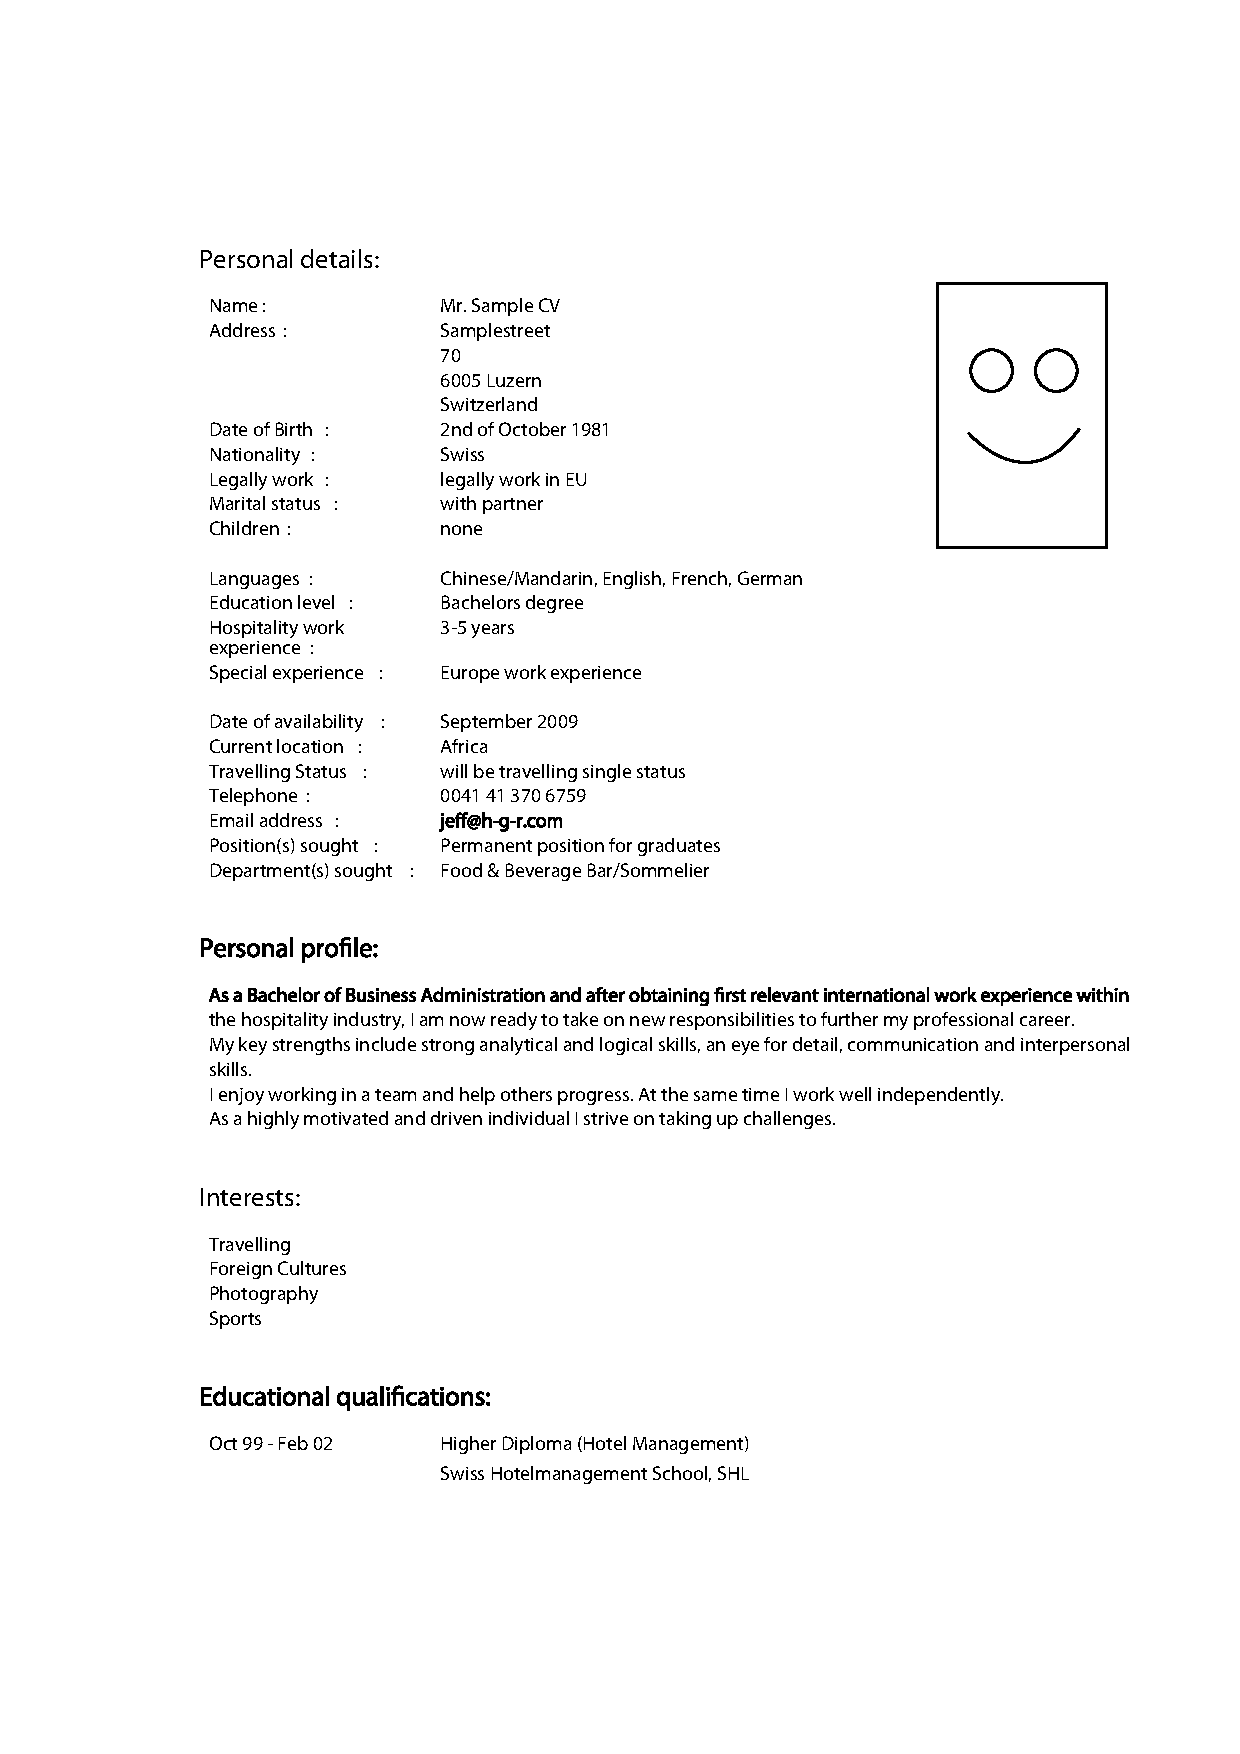
\includepdf[pagecommand=\thispagestyle{addpagenumbersforpdfimports},pages=-]{tail/cv/cv.pdf} % To upload a PDF CV directly
\subfile{tail/cv/cv_main.tex} % To do cv with LaTeX

\end{document}
